\title{A Very Simple \LaTeXe{} Template}
\author{
        Vitaly Surazhsky \\
                Department of Computer Science\\
        Technion---Israel Institute of Technology\\
        Technion City, Haifa 32000, \underline{Israel}
            \and
        Yossi Gil\\
        Department of Computer Science\\
        Technion---Israel Institute of Technology\\
        Technion City, Haifa 32000, \underline{Israel}
}
\date{\today}

\documentclass[12pt]{article}

\usepackage{makeidx}
\makeindex

%\documentclass{article}
\usepackage{fancyvrb}
\usepackage{color}
%\usepackage[utf-8]{inputenc}



\makeatletter
\def\PY@reset{\let\PY@it=\relax \let\PY@bf=\relax%
    \let\PY@ul=\relax \let\PY@tc=\relax%
    \let\PY@bc=\relax \let\PY@ff=\relax}
\def\PY@tok#1{\csname PY@tok@#1\endcsname}
\def\PY@toks#1+{\ifx\relax#1\empty\else%
    \PY@tok{#1}\expandafter\PY@toks\fi}
\def\PY@do#1{\PY@bc{\PY@tc{\PY@ul{%
    \PY@it{\PY@bf{\PY@ff{#1}}}}}}}
\def\PY#1#2{\PY@reset\PY@toks#1+\relax+\PY@do{#2}}

\def\PY@tok@gd{\def\PY@tc##1{\textcolor[rgb]{0.63,0.00,0.00}{##1}}}
\def\PY@tok@gu{\let\PY@bf=\textbf\def\PY@tc##1{\textcolor[rgb]{0.50,0.00,0.50}{##1}}}
\def\PY@tok@gt{\def\PY@tc##1{\textcolor[rgb]{0.00,0.25,0.82}{##1}}}
\def\PY@tok@gs{\let\PY@bf=\textbf}
\def\PY@tok@gr{\def\PY@tc##1{\textcolor[rgb]{1.00,0.00,0.00}{##1}}}
\def\PY@tok@cm{\let\PY@it=\textit\def\PY@tc##1{\textcolor[rgb]{0.25,0.50,0.50}{##1}}}
\def\PY@tok@vg{\def\PY@tc##1{\textcolor[rgb]{0.10,0.09,0.49}{##1}}}
\def\PY@tok@m{\def\PY@tc##1{\textcolor[rgb]{0.40,0.40,0.40}{##1}}}
\def\PY@tok@mh{\def\PY@tc##1{\textcolor[rgb]{0.40,0.40,0.40}{##1}}}
\def\PY@tok@go{\def\PY@tc##1{\textcolor[rgb]{0.50,0.50,0.50}{##1}}}
\def\PY@tok@ge{\let\PY@it=\textit}
\def\PY@tok@vc{\def\PY@tc##1{\textcolor[rgb]{0.10,0.09,0.49}{##1}}}
\def\PY@tok@il{\def\PY@tc##1{\textcolor[rgb]{0.40,0.40,0.40}{##1}}}
\def\PY@tok@cs{\let\PY@it=\textit\def\PY@tc##1{\textcolor[rgb]{0.25,0.50,0.50}{##1}}}
\def\PY@tok@cp{\def\PY@tc##1{\textcolor[rgb]{0.74,0.48,0.00}{##1}}}
\def\PY@tok@gi{\def\PY@tc##1{\textcolor[rgb]{0.00,0.63,0.00}{##1}}}
\def\PY@tok@gh{\let\PY@bf=\textbf\def\PY@tc##1{\textcolor[rgb]{0.00,0.00,0.50}{##1}}}
\def\PY@tok@ni{\let\PY@bf=\textbf\def\PY@tc##1{\textcolor[rgb]{0.60,0.60,0.60}{##1}}}
\def\PY@tok@nl{\def\PY@tc##1{\textcolor[rgb]{0.63,0.63,0.00}{##1}}}
\def\PY@tok@nn{\let\PY@bf=\textbf\def\PY@tc##1{\textcolor[rgb]{0.00,0.00,1.00}{##1}}}
\def\PY@tok@no{\def\PY@tc##1{\textcolor[rgb]{0.53,0.00,0.00}{##1}}}
\def\PY@tok@na{\def\PY@tc##1{\textcolor[rgb]{0.49,0.56,0.16}{##1}}}
\def\PY@tok@nb{\def\PY@tc##1{\textcolor[rgb]{0.00,0.50,0.00}{##1}}}
\def\PY@tok@nc{\let\PY@bf=\textbf\def\PY@tc##1{\textcolor[rgb]{0.00,0.00,1.00}{##1}}}
\def\PY@tok@nd{\def\PY@tc##1{\textcolor[rgb]{0.67,0.13,1.00}{##1}}}
\def\PY@tok@ne{\let\PY@bf=\textbf\def\PY@tc##1{\textcolor[rgb]{0.82,0.25,0.23}{##1}}}
\def\PY@tok@nf{\def\PY@tc##1{\textcolor[rgb]{0.00,0.00,1.00}{##1}}}
\def\PY@tok@si{\let\PY@bf=\textbf\def\PY@tc##1{\textcolor[rgb]{0.73,0.40,0.53}{##1}}}
\def\PY@tok@s2{\def\PY@tc##1{\textcolor[rgb]{0.73,0.13,0.13}{##1}}}
\def\PY@tok@vi{\def\PY@tc##1{\textcolor[rgb]{0.10,0.09,0.49}{##1}}}
\def\PY@tok@nt{\let\PY@bf=\textbf\def\PY@tc##1{\textcolor[rgb]{0.00,0.50,0.00}{##1}}}
\def\PY@tok@nv{\def\PY@tc##1{\textcolor[rgb]{0.10,0.09,0.49}{##1}}}
\def\PY@tok@s1{\def\PY@tc##1{\textcolor[rgb]{0.73,0.13,0.13}{##1}}}
\def\PY@tok@sh{\def\PY@tc##1{\textcolor[rgb]{0.73,0.13,0.13}{##1}}}
\def\PY@tok@sc{\def\PY@tc##1{\textcolor[rgb]{0.73,0.13,0.13}{##1}}}
\def\PY@tok@sx{\def\PY@tc##1{\textcolor[rgb]{0.00,0.50,0.00}{##1}}}
\def\PY@tok@bp{\def\PY@tc##1{\textcolor[rgb]{0.00,0.50,0.00}{##1}}}
\def\PY@tok@c1{\let\PY@it=\textit\def\PY@tc##1{\textcolor[rgb]{0.25,0.50,0.50}{##1}}}
\def\PY@tok@kc{\let\PY@bf=\textbf\def\PY@tc##1{\textcolor[rgb]{0.00,0.50,0.00}{##1}}}
\def\PY@tok@c{\let\PY@it=\textit\def\PY@tc##1{\textcolor[rgb]{0.25,0.50,0.50}{##1}}}
\def\PY@tok@mf{\def\PY@tc##1{\textcolor[rgb]{0.40,0.40,0.40}{##1}}}
\def\PY@tok@err{\def\PY@bc##1{\fcolorbox[rgb]{1.00,0.00,0.00}{1,1,1}{##1}}}
\def\PY@tok@kd{\let\PY@bf=\textbf\def\PY@tc##1{\textcolor[rgb]{0.00,0.50,0.00}{##1}}}
\def\PY@tok@ss{\def\PY@tc##1{\textcolor[rgb]{0.10,0.09,0.49}{##1}}}
\def\PY@tok@sr{\def\PY@tc##1{\textcolor[rgb]{0.73,0.40,0.53}{##1}}}
\def\PY@tok@mo{\def\PY@tc##1{\textcolor[rgb]{0.40,0.40,0.40}{##1}}}
\def\PY@tok@kn{\let\PY@bf=\textbf\def\PY@tc##1{\textcolor[rgb]{0.00,0.50,0.00}{##1}}}
\def\PY@tok@mi{\def\PY@tc##1{\textcolor[rgb]{0.40,0.40,0.40}{##1}}}
\def\PY@tok@gp{\let\PY@bf=\textbf\def\PY@tc##1{\textcolor[rgb]{0.00,0.00,0.50}{##1}}}
\def\PY@tok@o{\def\PY@tc##1{\textcolor[rgb]{0.40,0.40,0.40}{##1}}}
\def\PY@tok@kr{\let\PY@bf=\textbf\def\PY@tc##1{\textcolor[rgb]{0.00,0.50,0.00}{##1}}}
\def\PY@tok@s{\def\PY@tc##1{\textcolor[rgb]{0.73,0.13,0.13}{##1}}}
\def\PY@tok@kp{\def\PY@tc##1{\textcolor[rgb]{0.00,0.50,0.00}{##1}}}
\def\PY@tok@w{\def\PY@tc##1{\textcolor[rgb]{0.73,0.73,0.73}{##1}}}
\def\PY@tok@kt{\def\PY@tc##1{\textcolor[rgb]{0.69,0.00,0.25}{##1}}}
\def\PY@tok@ow{\let\PY@bf=\textbf\def\PY@tc##1{\textcolor[rgb]{0.67,0.13,1.00}{##1}}}
\def\PY@tok@sb{\def\PY@tc##1{\textcolor[rgb]{0.73,0.13,0.13}{##1}}}
\def\PY@tok@k{\let\PY@bf=\textbf\def\PY@tc##1{\textcolor[rgb]{0.00,0.50,0.00}{##1}}}
\def\PY@tok@se{\let\PY@bf=\textbf\def\PY@tc##1{\textcolor[rgb]{0.73,0.40,0.13}{##1}}}
\def\PY@tok@sd{\let\PY@it=\textit\def\PY@tc##1{\textcolor[rgb]{0.73,0.13,0.13}{##1}}}

\def\PYZbs{\char`\\}
\def\PYZus{\char`\_}
\def\PYZob{\char`\{}
\def\PYZcb{\char`\}}
\def\PYZca{\char`\^}
\def\PYZsh{\char`\#}
\def\PYZpc{\char`\%}
\def\PYZdl{\char`\$}
\def\PYZti{\char`\~}
% for compatibility with earlier versions
\def\PYZat{@}
\def\PYZlb{[}
\def\PYZrb{]}
\makeatother

\include{listings}

\usepackage{amsmath}

%for images
\usepackage{graphicx}

%for strike-through
\usepackage{ulem}
\usepackage[parfill]{parskip}

\begin{document}
\maketitle

\section{python}\index{python}

\subsection{Testing}\index{python!Testing}

A \textbf{Regression Test} tests that the output of some function does not change
when the program is refactored.

\scriptsize
\begin{Verbatim}[commandchars=\\\{\}]
\PY{k+kn}{import} \PY{n+nn}{time}

\PY{n}{examples} \PY{o}{=} \PY{l+s}{"""}\PY{l+s}{TWO + TWO == FOURi}
\PY{l+s}{A**2 + B**2 == C**2}\PY{l+s}{"""}\PY{o}{.}\PY{n}{splitlines}\PY{p}{(}\PY{p}{)}

\PY{k}{def} \PY{n+nf}{test}\PY{p}{(}\PY{p}{)}\PY{p}{:}
  \PY{n}{t0} \PY{o}{=} \PY{n}{time}\PY{o}{.}\PY{n}{clock}\PY{p}{(}\PY{p}{)}
  \PY{k}{for} \PY{n}{example} \PY{o+ow}{in} \PY{n}{examples}\PY{p}{:}
    \PY{k}{print}\PY{p}{;} \PY{k}{print} \PY{l+m+mi}{13}\PY{o}{*}\PY{l+s}{'}\PY{l+s}{ }\PY{l+s}{'}\PY{p}{,}\PY{n}{example}
    \PY{k}{print} \PY{l+s}{'}\PY{l+s+si}{\PYZpc{}6.4f}\PY{l+s}{ sec:   }\PY{l+s+si}{\PYZpc{}s}\PY{l+s}{ }\PY{l+s}{'} \PY{o}{\PYZpc{}} \PY{n}{timedcall}\PY{p}{(}\PY{n}{solve}\PY{p}{,} \PY{n}{example}\PY{p}{)}
  \PY{k}{print} \PY{l+s}{'}\PY{l+s+si}{\PYZpc{}6.4f}\PY{l+s}{ tot.}\PY{l+s}{'} \PY{o}{\PYZpc{}} \PY{p}{(}\PY{n}{time}\PY{o}{.}\PY{n}{clock}\PY{p}{(}\PY{p}{)}\PY{o}{-}\PY{n}{t0}\PY{p}{)}

\PY{n}{test}\PY{p}{(}\PY{p}{)}
\end{Verbatim}




\subsubsection{Dependency Injection}\index{python!Testing!Dependency Injection}

\begin{Verbatim}[commandchars=\\\{\}]
\PY{k+kn}{import} \PY{n+nn}{random}
\PY{k}{def} \PY{n+nf}{dierolls}\PY{p}{(}\PY{p}{)}\PY{p}{:}
  \PY{k}{while} \PY{n+nb+bp}{True}\PY{p}{:} \PY{k}{yield} \PY{n}{random}\PY{o}{.}\PY{n}{randint}\PY{p}{(}\PY{l+m+mi}{1}\PY{p}{,}\PY{l+m+mi}{6}\PY{p}{)}
\PY{k}{for} \PY{n}{\PYZus{}} \PY{o+ow}{in} \PY{n+nb}{range}\PY{p}{(}\PY{l+m+mi}{5}\PY{p}{)}\PY{p}{:} \PY{k}{print} \PY{n+nb}{next}\PY{p}{(}\PY{n}{dierolls}\PY{p}{(}\PY{p}{)}\PY{p}{)} \PY{c}{\PYZsh{}5 random numbers}
\end{Verbatim}




\subsubsection{Assertions}\index{python!Testing!Assertion}

\texttt{python -O} disables assertions


\subsection{Debugging}

\textbf{The Devil's Guide to Debugging} - \textit{Steve McConnell}

\begin{list}{*}{
\setlength{\itemsep}{0pt}
\setlength{\parsep}{0pt}
\setlength{\topsep}{0pt}
\setlength{\partopsep}{0pt}
\setlength{\leftmargin}{2em}
\setlength{\labelwidth}{1.5em}
\setlength{\labelsep}{0.5em}
}
\item Scatter output statements throughout the code. The more the better.
\item Debug the program into existence. Keep on adding and removing statements until something works.
\item Never back up earlier versions. Who can't remember what he or she did just 5 min ago?
\item Don't bother understanding what the program should do. If it's not obvious, make it obvious.
\item Don't waste time understanding the problem. Most problems are trivial, anyway.
\item Use the most obvious fix. Fix the symptom not the problem.
\end{list}



\subsection{Profiling}
\begin{Verbatim}[commandchars=\\\{\}]
\PY{c}{\PYZsh{}Terminal}
\PY{err}{\PYZdl{}} \PY{n}{python} \PY{o}{-}\PY{n}{m} \PY{n}{cProfile} \PY{n+nb}{file}\PY{o}{.}\PY{n}{py}

\PY{c}{\PYZsh{}From within python}
\PY{k+kn}{import} \PY{n+nn}{cProfile}
\PY{n}{cProfile}\PY{o}{.}\PY{n}{run}\PY{p}{(}\PY{l+s}{'}\PY{l+s}{function()}\PY{l+s}{'}\PY{p}{)}
\end{Verbatim}


\subsection{string}\index{python!string}

\subsubsection{Substitution}\index{python!string!Substitution}

\begin{Verbatim}[commandchars=\\\{\}]
\PY{n}{s} \PY{o}{=} \PY{l+s}{"}\PY{l+s}{some bold}\PY{l+s}{"}
\PY{k}{print} \PY{l+s}{"}\PY{l+s}{<b>}\PY{l+s+si}{\PYZpc{}s}\PY{l+s}{</b> text}\PY{l+s}{"} \PY{o}{\PYZpc{}} \PY{n}{s}
\PY{c}{\PYZsh{}--> <b>some bold</b> text}
\PY{n}{s2} \PY{o}{=} \PY{l+s}{"}\PY{l+s}{some italic}\PY{l+s}{"}
\PY{k}{print} \PY{l+s}{"}\PY{l+s}{<b>}\PY{l+s+si}{\PYZpc{}s}\PY{l+s}{</b> and <i>}\PY{l+s+si}{\PYZpc{}s}\PY{l+s}{</i> text}\PY{l+s}{"} \PY{o}{\PYZpc{}} \PY{p}{(}\PY{n}{s}\PY{p}{,}\PY{n}{s2}\PY{p}{)}
\PY{c}{\PYZsh{}--> <b>some bold</b> and <i>some italic</i> text}
\PY{k}{print} \PY{l+s}{"}\PY{l+s}{I}\PY{l+s}{'}\PY{l+s}{m }\PY{l+s+si}{\PYZpc{}(nickname)s}\PY{l+s}{. My real name is }\PY{l+s+si}{\PYZpc{}(name)s}\PY{l+s}{, but my friends call me }\PY{l+s+si}{\PYZpc{}(nickname)s}\PY{l+s}{.}\PY{l+s}{"} \PY{o}{\PYZpc{}} \PY{p}{\PYZob{}}\PY{l+s}{'}\PY{l+s}{name}\PY{l+s}{'}\PY{p}{:}\PY{l+s}{'}\PY{l+s}{Mike}\PY{l+s}{'}\PY{p}{,}\PY{l+s}{'}\PY{l+s}{nickname}\PY{l+s}{'}\PY{p}{:}\PY{l+s}{'}\PY{l+s}{Goose}\PY{l+s}{'}\PY{p}{\PYZcb{}}
\PY{c}{\PYZsh{}--> I'm Goose. My real name is Mike, but my friends call me Goose.}
\end{Verbatim}


\subsubsection{split}\index{python!string!split}
\begin{Verbatim}[commandchars=\\\{\}]
\PY{c}{\PYZsh{}splitting by whitespace}
\PY{l+s}{"}\PY{l+s}{python is kind of fun}\PY{l+s}{"}\PY{o}{.}\PY{n}{split}\PY{p}{(}\PY{p}{)}
\end{Verbatim}


	

\subsection{hash}\index{python!hash}

Implements a hash function, that is irreversible, gives a unique output and changing the input just a litte, gives a totally different output.

\begin{list}{*}{
\setlength{\itemsep}{0pt}
\setlength{\parsep}{0pt}
\setlength{\topsep}{0pt}
\setlength{\partopsep}{0pt}
\setlength{\leftmargin}{2em}
\setlength{\labelwidth}{1.5em}
\setlength{\labelsep}{0.5em}
}
\item \textbf{crc32} - Designed for checksums. It's fast, but its security properties are not very good - it's very easy to find a \emph{collision}, when two things hash to the same value.
\item \textbf{md5} - Used to be used because it was pretty fast and pretty secured. But it's not secure any longer - it's easy to find collisions. It's found on every system.
\item \textbf{sha1} - Not as fast, but fairly secured. Second most widely used hash after md5.
\item \textbf{sha256} - If you are really worried about securing your data, but it's the slowest.
\item \textbf{bcrypt} - Besides incorporating a salt to protect against rainbow table attacks, bcrypt is an adaptive hash: over time it can be made slower and slower so it remains resistant to specific brute-force search attacks against the hash and the salt.
\end{list}

\subsubsection{get}\index{python!hash!get}

Does not generate a \emph{KeyError} when referencing a key that does not exist in the hash, unlike using the sqare brackets.

\begin{Verbatim}[commandchars=\\\{\}]
\PY{n}{h} \PY{o}{=} \PY{p}{\PYZob{}}\PY{l+s}{'}\PY{l+s}{ruby}\PY{l+s}{'}\PY{p}{:}\PY{l+s}{'}\PY{l+s}{rocks}\PY{l+s}{'}\PY{p}{\PYZcb{}}
\PY{n}{h}\PY{o}{.}\PY{n}{get}\PY{p}{(}\PY{l+s}{'}\PY{l+s}{python}\PY{l+s}{'}\PY{p}{)}
\PY{c}{\PYZsh{}--> <nothing>}
\PY{n}{h}\PY{p}{[}\PY{l+s}{'}\PY{l+s}{python}\PY{l+s}{'}\PY{p}{]}
\PY{c}{\PYZsh{}--> KeyError: 'python'}
\end{Verbatim}



\subsubsection{defaultdict}\index{python!hash!defaultdict}

\begin{Verbatim}[commandchars=\\\{\}]
\PY{k+kn}{from} \PY{n+nn}{collections} \PY{k+kn}{import} \PY{n}{defaultdict}
\PY{n}{cache} \PY{o}{=} \PY{n}{defaultdict}\PY{p}{(}\PY{n+nb}{int}\PY{p}{)}
\PY{k}{for} \PY{n}{c} \PY{o+ow}{in} \PY{l+s}{'}\PY{l+s}{abcd}\PY{l+s}{'}\PY{p}{:}
  \PY{n}{cache}\PY{p}{[}\PY{n}{c}\PY{p}{]} \PY{o}{+}\PY{o}{=} \PY{l+m+mi}{1}
\PY{k}{print} \PY{n}{cache} \PY{c}{\PYZsh{}--> defaultdict(<type 'int'>, \PYZob{}'a': 1, 'c': 1, 'b': 1, 'd': 1\PYZcb{})}
\end{Verbatim}



\subsubsection{merge}\index{python!hash!merge}

Merge two or more dictionaries

\begin{Verbatim}[commandchars=\\\{\}]
\PY{n}{a} \PY{o}{=} \PY{p}{\PYZob{}}\PY{l+s}{'}\PY{l+s}{a}\PY{l+s}{'}\PY{p}{:}\PY{l+m+mi}{1}\PY{p}{\PYZcb{}}\PY{p}{;} \PY{n}{b} \PY{o}{=} \PY{p}{\PYZob{}}\PY{l+s}{'}\PY{l+s}{b}\PY{l+s}{'}\PY{p}{:}\PY{l+m+mi}{2}\PY{p}{\PYZcb{}}
\PY{k}{print} \PY{n+nb}{dict}\PY{p}{(}\PY{n}{a}\PY{o}{.}\PY{n}{items}\PY{p}{(}\PY{p}{)}\PY{o}{+}\PY{n}{b}\PY{o}{.}\PY{n}{items}\PY{p}{(}\PY{p}{)}\PY{p}{)} \PY{c}{\PYZsh{}--> \PYZob{}'a': 1, 'b': 2\PYZcb{}}
\end{Verbatim}




\subsection{Lists}\index{python!Lists}


\subsubsection{map}\index{python!Lists!map}

\begin{Verbatim}[commandchars=\\\{\}]
\PY{n}{numbers} \PY{o}{=} \PY{p}{[}\PY{l+m+mi}{1}\PY{p}{,}\PY{l+m+mi}{2}\PY{p}{,}\PY{l+m+mi}{3}\PY{p}{]}
\PY{k}{def} \PY{n+nf}{mysquare}\PY{p}{(}\PY{n}{x}\PY{p}{)}\PY{p}{:} \PY{k}{return} \PY{n}{x}\PY{o}{*}\PY{n}{x}
\PY{k}{print} \PY{n+nb}{map}\PY{p}{(}\PY{n}{mysquare}\PY{p}{,}\PY{p}{[}\PY{l+m+mi}{1}\PY{p}{,}\PY{l+m+mi}{2}\PY{p}{,}\PY{l+m+mi}{3}\PY{p}{]}\PY{p}{)} \PY{c}{\PYZsh{}-->[1, 4, 9]}

\PY{c}{\PYZsh{}lambda below is called an anonymous function}
\PY{k}{print} \PY{n+nb}{map}\PY{p}{(}\PY{k}{lambda}\PY{p}{(}\PY{n}{x}\PY{p}{)}\PY{p}{:}\PY{n}{x}\PY{o}{*}\PY{n}{x}\PY{p}{,}\PY{p}{[}\PY{l+m+mi}{1}\PY{p}{,}\PY{l+m+mi}{2}\PY{p}{,}\PY{l+m+mi}{3}\PY{p}{]}\PY{p}{)} \PY{c}{\PYZsh{}-->[1, 4, 9]}

\PY{c}{\PYZsh{}list comprehension}
\PY{k}{print} \PY{p}{[}\PY{n}{x}\PY{o}{*}\PY{n}{x} \PY{k}{for} \PY{n}{x} \PY{o+ow}{in} \PY{p}{[}\PY{l+m+mi}{1}\PY{p}{,}\PY{l+m+mi}{2}\PY{p}{,}\PY{l+m+mi}{3}\PY{p}{]}\PY{p}{]} \PY{c}{\PYZsh{}-->[1, 4, 9]}

\PY{k}{def} \PY{n+nf}{map\PYZus{}maker1}\PY{p}{(}\PY{n}{f}\PY{p}{)}\PY{p}{:} \PY{k}{return} \PY{k}{lambda}\PY{p}{(}\PY{n}{a}\PY{p}{)}\PY{p}{:}\PY{p}{[}\PY{n}{f}\PY{p}{(}\PY{n}{e}\PY{p}{)} \PY{k}{for} \PY{n}{e} \PY{o+ow}{in} \PY{n}{a}\PY{p}{]}
\PY{n}{square\PYZus{}map} \PY{o}{=} \PY{n}{map\PYZus{}maker1}\PY{p}{(}\PY{k}{lambda}\PY{p}{(}\PY{n}{x}\PY{p}{)}\PY{p}{:}\PY{n}{x}\PY{o}{*}\PY{n}{x}\PY{p}{)}
\PY{k}{print} \PY{n}{square\PYZus{}map}\PY{p}{(}\PY{n}{numbers}\PY{p}{)} \PY{c}{\PYZsh{}--> [1, 4, 9]}

\PY{k}{def} \PY{n+nf}{map\PYZus{}maker2}\PY{p}{(}\PY{n}{f}\PY{p}{)}\PY{p}{:}
  \PY{k}{def} \PY{n+nf}{inner\PYZus{}map}\PY{p}{(}\PY{n}{a}\PY{p}{)}\PY{p}{:} \PY{k}{return} \PY{n+nb}{map}\PY{p}{(}\PY{n}{f}\PY{p}{,}\PY{n}{a}\PY{p}{)}
  \PY{k}{return} \PY{n}{inner\PYZus{}map}
\PY{n}{square\PYZus{}map} \PY{o}{=} \PY{n}{map\PYZus{}maker2}\PY{p}{(}\PY{k}{lambda}\PY{p}{(}\PY{n}{x}\PY{p}{)}\PY{p}{:}\PY{n}{x}\PY{o}{*}\PY{n}{x}\PY{p}{)}
\PY{k}{print} \PY{n}{square\PYZus{}map}\PY{p}{(}\PY{n}{numbers}\PY{p}{)} \PY{c}{\PYZsh{}--> [1, 4, 9]}
\end{Verbatim}



\subsubsection{filter}\index{python!Lists!filter}

\begin{Verbatim}[commandchars=\\\{\}]
\PY{c}{\PYZsh{}anonymous function}
\PY{n}{numbers} \PY{o}{=} \PY{p}{[}\PY{l+m+mi}{1}\PY{p}{,}\PY{l+m+mi}{2}\PY{p}{,}\PY{l+m+mi}{3}\PY{p}{,}\PY{l+m+mi}{4}\PY{p}{]}
\PY{k}{print} \PY{n+nb}{filter}\PY{p}{(}\PY{k}{lambda}\PY{p}{(}\PY{n}{x}\PY{p}{)}\PY{p}{:}\PY{n}{x}\PY{o}{\PYZpc{}}\PY{l+m+mi}{2}\PY{o}{==}\PY{l+m+mi}{1}\PY{p}{,} \PY{n}{numbers}\PY{p}{)} \PY{c}{\PYZsh{}--> [1, 3]}

\PY{c}{\PYZsh{}list comprehension}
\PY{k}{print} \PY{p}{[}\PY{n}{x} \PY{k}{for} \PY{n}{x} \PY{o+ow}{in} \PY{n}{numbers} \PY{k}{if} \PY{n}{x}\PY{o}{\PYZpc{}}\PY{l+m+mi}{2}\PY{o}{==}\PY{l+m+mi}{1}\PY{p}{]} \PY{c}{\PYZsh{}--> [1, 3]}

\PY{k}{def} \PY{n+nf}{filter\PYZus{}maker1}\PY{p}{(}\PY{n}{f}\PY{p}{)}\PY{p}{:} \PY{k}{return} \PY{k}{lambda} \PY{n}{a}\PY{p}{:}\PY{p}{[}\PY{n}{e} \PY{k}{for} \PY{n}{e} \PY{o+ow}{in} \PY{n}{a} \PY{k}{if} \PY{n}{f}\PY{p}{(}\PY{n}{e}\PY{p}{)}\PY{p}{]}
\PY{n}{filter\PYZus{}odds} \PY{o}{=} \PY{n}{filter\PYZus{}maker1}\PY{p}{(}\PY{k}{lambda}\PY{p}{(}\PY{n}{x}\PY{p}{)}\PY{p}{:}\PY{n}{x}\PY{o}{\PYZpc{}}\PY{l+m+mi}{2}\PY{o}{==}\PY{l+m+mi}{1}\PY{p}{)}
\PY{k}{print} \PY{n}{filter\PYZus{}odds}\PY{p}{(}\PY{n}{numbers}\PY{p}{)} \PY{c}{\PYZsh{}--> [1, 3]}

\PY{k}{def} \PY{n+nf}{filter\PYZus{}maker2}\PY{p}{(}\PY{n}{f}\PY{p}{)}\PY{p}{:}
  \PY{k}{def} \PY{n+nf}{inner\PYZus{}filter}\PY{p}{(}\PY{n}{a}\PY{p}{)}\PY{p}{:} \PY{k}{return} \PY{n+nb}{filter}\PY{p}{(}\PY{n}{f}\PY{p}{,}\PY{n}{a}\PY{p}{)}
  \PY{k}{return} \PY{n}{inner\PYZus{}filter}
\PY{n}{filter\PYZus{}odds} \PY{o}{=} \PY{n}{filter\PYZus{}maker2}\PY{p}{(}\PY{k}{lambda}\PY{p}{(}\PY{n}{x}\PY{p}{)}\PY{p}{:}\PY{n}{x}\PY{o}{\PYZpc{}}\PY{l+m+mi}{2}\PY{o}{==}\PY{l+m+mi}{1}\PY{p}{)}
\PY{k}{print} \PY{n}{filter\PYZus{}odds}\PY{p}{(}\PY{n}{numbers}\PY{p}{)} \PY{c}{\PYZsh{}--> [1, 3]}
\end{Verbatim}


\begin{Verbatim}[commandchars=\\\{\}]
\PY{n}{l} \PY{o}{=} \PY{p}{[}\PY{l+m+mi}{1}\PY{p}{,} \PY{n+nb+bp}{None}\PY{p}{,} \PY{l+m+mi}{2}\PY{p}{]}
\PY{l+s+sd}{"""filter return all the items in the list that match the function.}
\PY{l+s+sd}{   if there is no function, match all that are not None"""}
\PY{k}{print} \PY{n+nb}{filter}\PY{p}{(}\PY{n+nb+bp}{None}\PY{p}{,} \PY{p}{(}\PY{n}{e} \PY{k}{for} \PY{n}{e} \PY{o+ow}{in} \PY{n}{l}\PY{p}{)}\PY{p}{)} \PY{c}{\PYZsh{}--> [1, 2] }
\end{Verbatim}



\subsubsection{sorted}\index{python!Lists!sorted}

\begin{Verbatim}[commandchars=\\\{\}]
\PY{k}{print} \PY{n+nb}{sorted}\PY{p}{(}\PY{p}{[}\PY{l+s}{'}\PY{l+s}{a}\PY{l+s}{'}\PY{p}{,}\PY{l+s}{'}\PY{l+s}{bc}\PY{l+s}{'}\PY{p}{]}\PY{p}{,} \PY{n}{reverse} \PY{o}{=} \PY{n+nb+bp}{True}\PY{p}{)} \PY{c}{\PYZsh{} --> ['bc', 'a']}
\PY{k}{print} \PY{n+nb}{sorted}\PY{p}{(}\PY{p}{[}\PY{l+s}{'}\PY{l+s}{a}\PY{l+s}{'}\PY{p}{,}\PY{l+s}{'}\PY{l+s}{bc}\PY{l+s}{'}\PY{p}{]}\PY{p}{,} \PY{n}{key} \PY{o}{=} \PY{n+nb}{len}\PY{p}{)}      \PY{c}{\PYZsh{} --> ['a', 'bc']}
\end{Verbatim}



\subsubsection{Selecting certain values}\index{python!Lists!Selecting_certain_values}

\begin{Verbatim}[commandchars=\\\{\}]
\PY{k+kn}{import} \PY{n+nn}{operator}
\PY{k}{print} \PY{n}{operator}\PY{o}{.}\PY{n}{itemgetter}\PY{p}{(}\PY{l+m+mi}{0}\PY{p}{,}\PY{l+m+mi}{2}\PY{p}{)}\PY{p}{(}\PY{p}{[}\PY{l+m+mi}{0}\PY{p}{,}\PY{l+m+mi}{1}\PY{p}{,}\PY{l+m+mi}{2}\PY{p}{]}\PY{p}{)} \PY{c}{\PYZsh{}--> (0,2)}
\end{Verbatim}




\subsection{Files}\index{python!Files}




\subsection{itertools}\index{python!itertools}

\subsubsection{permutations}
\begin{Verbatim}[commandchars=\\\{\}]
\PY{k+kn}{import} \PY{n+nn}{itertools}

\PY{c}{\PYZsh{}In how many ways can five numbers be ordered?}
\PY{n}{orderings} \PY{o}{=} \PY{n+nb}{list}\PY{p}{(}\PY{n}{itertools}\PY{o}{.}\PY{n}{permutations}\PY{p}{(}\PY{p}{[}\PY{l+m+mi}{1}\PY{p}{,}\PY{l+m+mi}{2}\PY{p}{,}\PY{l+m+mi}{3}\PY{p}{,}\PY{l+m+mi}{4}\PY{p}{,}\PY{l+m+mi}{5}\PY{p}{]}\PY{p}{)}\PY{p}{)}
\PY{k}{print} \PY{n+nb}{len}\PY{p}{(}\PY{n}{orderings}\PY{p}{)}
\PY{c}{\PYZsh{}--> 120}

\PY{c}{\PYZsh{}In how many ways can ten numbers be ordered in groups of three?}
\PY{n}{orderings} \PY{o}{=} \PY{n+nb}{list}\PY{p}{(}\PY{n}{itertools}\PY{o}{.}\PY{n}{permutations}\PY{p}{(}\PY{l+s}{'}\PY{l+s}{1234567890}\PY{l+s}{'}\PY{p}{,}\PY{l+m+mi}{3}\PY{p}{)}\PY{p}{)}
\PY{k}{print} \PY{n+nb}{len}\PY{p}{(}\PY{n}{orderings}\PY{p}{)}
\PY{c}{\PYZsh{}--> 720}
\end{Verbatim}





\subsection{random}\index{python!random}


\subsubsection{choice}\index/{python!random!choice}

\begin{Verbatim}[commandchars=\\\{\}]
\PY{k+kn}{import} \PY{n+nn}{string}
\PY{k+kn}{import} \PY{n+nn}{random}
\PY{k+kn}{import} \PY{n+nn}{doctest}
\PY{k}{def} \PY{n+nf}{make\PYZus{}salt}\PY{p}{(}\PY{p}{)}\PY{p}{:}
  \PY{l+s+sd}{"""5 random characters}
\PY{l+s+sd}{  >>> len(make\PYZus{}salt())}
\PY{l+s+sd}{  5}
\PY{l+s+sd}{  """}
  \PY{k}{return} \PY{l+s}{"}\PY{l+s}{"}\PY{o}{.}\PY{n}{join}\PY{p}{(}\PY{n}{random}\PY{o}{.}\PY{n}{choice}\PY{p}{(}\PY{n}{string}\PY{o}{.}\PY{n}{letters}\PY{p}{)} \PY{k}{for} \PY{n}{\PYZus{}} \PY{o+ow}{in} \PY{n+nb}{xrange}\PY{p}{(}\PY{l+m+mi}{5}\PY{p}{)}\PY{p}{)}
\PY{k}{print} \PY{n}{doctest}\PY{o}{.}\PY{n}{testmod}\PY{p}{(}\PY{p}{)}
\end{Verbatim}


A strategy that chooses at random from possible moves.

\begin{Verbatim}[commandchars=\\\{\}]
\PY{k+kn}{import} \PY{n+nn}{random}
\PY{n}{possible\PYZus{}moves} \PY{o}{=} \PY{p}{[}\PY{l+s}{'}\PY{l+s}{roll}\PY{l+s}{'}\PY{p}{,}\PY{l+s}{'}\PY{l+s}{hold}\PY{l+s}{'}\PY{p}{]}
\PY{k}{def} \PY{n+nf}{clueless}\PY{p}{(}\PY{p}{)}\PY{p}{:} \PY{k}{return} \PY{n}{random}\PY{o}{.}\PY{n}{choice}\PY{p}{(}\PY{n}{possible\PYZus{}moves}\PY{p}{)}
\end{Verbatim}



\subsubsection{randint}\index{python!random!randint}

\begin{Verbatim}[commandchars=\\\{\}]
\PY{k+kn}{import} \PY{n+nn}{random}
\PY{n}{random}\PY{o}{.}\PY{n}{randint}\PY{p}{(}\PY{l+m+mi}{1}\PY{p}{,}\PY{l+m+mi}{6}\PY{p}{)} \PY{c}{\PYZsh{}output from 1 to 6}
\end{Verbatim}




\subsection{json}\index{python!json}

\subsubsection{loads - load string}\index{python!json!loads}

\begin{Verbatim}[commandchars=\\\{\}]
\PY{k+kn}{import} \PY{n+nn}{json}
\PY{n}{json\PYZus{}string} \PY{o}{=} \PY{l+s}{'}\PY{l+s}{\PYZob{}}\PY{l+s}{"}\PY{l+s}{json}\PY{l+s}{"}\PY{l+s}{:}\PY{l+s}{"}\PY{l+s}{string}\PY{l+s}{"}\PY{l+s}{\PYZcb{}}\PY{l+s}{'}
\PY{n}{j} \PY{o}{=} \PY{n}{json}\PY{o}{.}\PY{n}{loads}\PY{p}{(}\PY{n}{json\PYZus{}string}\PY{p}{)}
\PY{k}{print} \PY{n}{j}\PY{p}{[}\PY{l+s}{'}\PY{l+s}{json}\PY{l+s}{'}\PY{p}{]} \PY{c}{\PYZsh{}--> string}
\end{Verbatim}



\subsubsection{dumps - dump string}\index{python!json!dumps}

Json has to use double quotes to delineate a string.

\begin{Verbatim}[commandchars=\\\{\}]
\PY{k+kn}{import} \PY{n+nn}{json}
\PY{k}{print} \PY{n}{json}\PY{o}{.}\PY{n}{dumps}\PY{p}{(}\PY{p}{\PYZob{}}\PY{l+s}{"}\PY{l+s}{one}\PY{l+s}{"}\PY{p}{:}\PY{l+m+mi}{1}\PY{p}{,} \PY{l+s}{"}\PY{l+s}{two}\PY{l+s}{"}\PY{p}{:}\PY{l+s}{'}\PY{l+s}{the man said, }\PY{l+s}{"}\PY{l+s}{cool!}\PY{l+s}{"}\PY{l+s}{'}\PY{p}{\PYZcb{}}\PY{p}{)}
\PY{c}{\PYZsh{}--> \PYZob{}"two": "the man said, \PYZbs{}"cool!\PYZbs{}"", "one": 1\PYZcb{}}
\end{Verbatim}




\subsection{xml}\index{python!xml}AttributeError: 'module' object has no attribute 'urlopen'

\subsubsection{minidom}\index{python!xml!minidom}

\begin{Verbatim}[commandchars=\\\{\}]
\PY{k+kn}{from} \PY{n+nn}{xml.dom} \PY{k+kn}{import} \PY{n}{minidom}
\PY{n}{xml} \PY{o}{=} \PY{l+s}{"""}\PY{l+s}{<xml>}
\PY{l+s}{  <li>List 1</li>}
\PY{l+s}{  <li>List 2</li>}
\PY{l+s}{</xml>}\PY{l+s}{"""}
\PY{n}{d} \PY{o}{=} \PY{n}{minidom}\PY{o}{.}\PY{n}{parseString}\PY{p}{(}\PY{n}{xml}\PY{p}{)}
\PY{k}{print} \PY{p}{[}\PY{n}{e}\PY{o}{.}\PY{n}{childNodes}\PY{p}{[}\PY{l+m+mi}{0}\PY{p}{]}\PY{o}{.}\PY{n}{nodeValue} \PY{k}{for} \PY{n}{e} \PY{o+ow}{in} \PY{n}{d}\PY{o}{.}\PY{n}{getElementsByTagName}\PY{p}{(}\PY{l+s}{"}\PY{l+s}{li}\PY{l+s}{"}\PY{p}{)}\PY{p}{]}
\PY{c}{\PYZsh{}--> [u'List 1', u'List 2']}
\end{Verbatim}




\subsection{urllib2}

\begin{Verbatim}[commandchars=\\\{\}]
\PY{k+kn}{import} \PY{n+nn}{urllib2}
\PY{n}{url} \PY{o}{=} \PY{l+s}{"}\PY{l+s}{http://api.hostip.info/?ip=4.2.2.2}\PY{l+s}{"}
\PY{n}{urllib2}\PY{o}{.}\PY{n}{urlopen}\PY{p}{(}\PY{n}{url}\PY{p}{)}\PY{o}{.}\PY{n}{read}\PY{p}{(}\PY{p}{)}
\end{Verbatim}




\subsection{Exceptions}\index{python!Exceptions}

\begin{Verbatim}[commandchars=\\\{\}]
\PY{k}{try}\PY{p}{:}
  \PY{k}{print} \PY{l+s}{"}\PY{l+s}{one}\PY{l+s}{"} \PY{c}{\PYZsh{}--> one}
  \PY{k}{raise} \PY{n+ne}{Exception}\PY{p}{(}\PY{l+s}{"}\PY{l+s}{three}\PY{l+s}{"}\PY{p}{)}
  \PY{k}{print} \PY{l+s}{"}\PY{l+s}{two}\PY{l+s}{"}
\PY{k}{except} \PY{n+ne}{Exception} \PY{k}{as} \PY{n}{problem}\PY{p}{:}
  \PY{k}{print} \PY{n}{problem} \PY{c}{\PYZsh{}--> three}
\end{Verbatim}





\subsection{range vs xrange}\index{python!range}\index{python!xrange}

range creates a list in memory, but xrange is a generator, so it evaluates lazily.



\subsection{Variables}\index{python!Variables}

\subsubsection{Global}\index{python!Variables!Global}

Local variables overrides a global of the same name. To prevent that behaviour and
to be able to modify the variable within a function, python must be told to use the
name in a global sense.

\begin{Verbatim}[commandchars=\\\{\}]
\PY{n}{god} \PY{o}{=} \PY{l+m+mi}{1}
\PY{k}{def} \PY{n+nf}{local\PYZus{}func}\PY{p}{(}\PY{p}{)}\PY{p}{:}
  \PY{k}{global} \PY{n}{god}
  \PY{n}{god} \PY{o}{=} \PY{l+m+mi}{2}
  \PY{k}{print} \PY{n}{god}
\PY{n}{local\PYZus{}func}\PY{p}{(}\PY{p}{)}
\PY{k}{print} \PY{n}{god}
\end{Verbatim}



\subsection{lambda}

\begin{Verbatim}[commandchars=\\\{\}]
\PY{n}{mystery} \PY{o}{=} \PY{k}{lambda}\PY{p}{(}\PY{n}{x}\PY{p}{)}\PY{p}{:}\PY{n}{x}\PY{o}{+}\PY{l+m+mi}{2}
\PY{k}{print} \PY{n}{mystery}\PY{p}{(}\PY{l+m+mi}{3}\PY{p}{)} \PY{c}{\PYZsh{}-->5}
\end{Verbatim}



\subsection{Internal methods}

\subsubsection{\_\_name\_\_}

\begin{Verbatim}[commandchars=\\\{\}]
\PY{k}{def} \PY{n+nf}{debug\PYZus{}fn}\PY{p}{(}\PY{n}{f}\PY{p}{)}\PY{p}{:}
  \PY{l+s+sd}{"""Return a modified function that first prints out }
\PY{l+s+sd}{  function name and arguments}
\PY{l+s+sd}{  then calls the function."""} \PY{c}{\PYZsh{} this is the doc string}
  \PY{k}{def} \PY{n+nf}{\PYZus{}f}\PY{p}{(}\PY{o}{*}\PY{n}{args}\PY{p}{)}\PY{p}{:}
      \PY{l+s+sd}{""" Here's the bit that prints out the name and args"""}
      \PY{k}{print} \PY{l+s}{"}\PY{l+s}{Called }\PY{l+s+si}{\PYZpc{}s}\PY{l+s}{(}\PY{l+s+si}{\PYZpc{}s}\PY{l+s}{)}\PY{l+s}{"}\PY{o}{\PYZpc{}}\PY{p}{(}\PY{n}{f}\PY{o}{.}\PY{n}{\PYZus{}\PYZus{}name\PYZus{}\PYZus{}}\PY{p}{,} \PY{l+s}{'}\PY{l+s}{, }\PY{l+s}{'}\PY{o}{.}\PY{n}{join}\PY{p}{(}\PY{n+nb}{map}\PY{p}{(}\PY{n+nb}{repr}\PY{p}{,} \PY{n}{args}\PY{p}{)}\PY{p}{)}\PY{p}{)}
      \PY{k}{return} \PY{n}{f}\PY{p}{(}\PY{o}{*}\PY{n}{args}\PY{p}{)}
  \PY{k}{return} \PY{n}{\PYZus{}f}

\PY{k}{print} \PY{n}{debug\PYZus{}fn}\PY{o}{.}\PY{n}{\PYZus{}\PYZus{}name\PYZus{}\PYZus{}}
\PY{c}{\PYZsh{} --> debug\PYZus{}fn}
\end{Verbatim}


\subsubsection{\_\_doc\_\_}

\begin{Verbatim}[commandchars=\\\{\}]
\PY{k}{print} \PY{n}{debug\PYZus{}fn}\PY{o}{.}\PY{n}{\PYZus{}\PYZus{}doc\PYZus{}\PYZus{}}
\PY{c}{\PYZsh{} --> Return a modified function that first prints out }
\PY{c}{\PYZsh{} -->   function name and arguments}
\PY{c}{\PYZsh{} -->   then calls the function.}
\end{Verbatim}


\subsubsection{\_\_repr\_\_}

The representation method is called whenever an object of the particular class is to be printed and returns a string representation of the object.



\subsection{Classes}

\begin{Verbatim}[commandchars=\\\{\}]
\PY{k+kn}{from} \PY{n+nn}{collections} \PY{k+kn}{import} \PY{n}{namedtuple}
\PY{n}{Link} \PY{o}{=} \PY{n}{namedtuple}\PY{p}{(}\PY{l+s}{'}\PY{l+s}{Link}\PY{l+s}{'}\PY{p}{,}\PY{p}{[}\PY{l+s}{'}\PY{l+s}{id}\PY{l+s}{'}\PY{p}{,}\PY{l+s}{'}\PY{l+s}{url}\PY{l+s}{'}\PY{p}{]}\PY{p}{)}
\PY{k}{print} \PY{n}{Link}\PY{p}{(}\PY{l+m+mi}{1}\PY{p}{,}\PY{l+s}{'}\PY{l+s}{google.com}\PY{l+s}{'}\PY{p}{)} \PY{c}{\PYZsh{}--> Link(id=1, url='google.com')}
\end{Verbatim}



\subsection{Structured Query Language - SQL}\index{SQL}

Invented in the 1970s.

\begin{Verbatim}[commandchars=\\\{\}]
\PY{k+kn}{import} \PY{n+nn}{sqlite3}
\PY{k+kn}{from} \PY{n+nn}{collections} \PY{k+kn}{import} \PY{n}{namedtuple}
\PY{n}{Link} \PY{o}{=} \PY{n}{namedtuple}\PY{p}{(}\PY{l+s}{'}\PY{l+s}{Link}\PY{l+s}{'}\PY{p}{,}\PY{p}{[}\PY{l+s}{'}\PY{l+s}{id}\PY{l+s}{'}\PY{p}{,}\PY{l+s}{'}\PY{l+s}{url}\PY{l+s}{'}\PY{p}{]}\PY{p}{)}

\PY{n}{db} \PY{o}{=} \PY{n}{sqlite3}\PY{o}{.}\PY{n}{connect}\PY{p}{(}\PY{l+s}{'}\PY{l+s}{:memory:}\PY{l+s}{'}\PY{p}{)}
\PY{n}{db}\PY{o}{.}\PY{n}{execute}\PY{p}{(}\PY{l+s}{'}\PY{l+s}{create table links (id integer, url text)}\PY{l+s}{'}\PY{p}{)}
\PY{n}{db}\PY{o}{.}\PY{n}{execute}\PY{p}{(}\PY{l+s}{'}\PY{l+s}{insert into links values (?,?)}\PY{l+s}{'}\PY{p}{,}\PY{n}{Link}\PY{p}{(}\PY{l+m+mi}{1}\PY{p}{,}\PY{l+s}{'}\PY{l+s}{google.com}\PY{l+s}{'}\PY{p}{)}\PY{p}{)}
\PY{n}{cursor} \PY{o}{=} \PY{n}{db}\PY{o}{.}\PY{n}{execute}\PY{p}{(}\PY{l+s}{'}\PY{l+s}{select url from links}\PY{l+s}{'}\PY{p}{)}
\PY{k}{for} \PY{n}{link\PYZus{}tuple} \PY{o+ow}{in} \PY{n}{cursor}\PY{p}{:}
  \PY{k}{print} \PY{n}{link\PYZus{}tuple} \PY{c}{\PYZsh{}--> (u'google.com',)}
\PY{n}{cursor} \PY{o}{=} \PY{n}{db}\PY{o}{.}\PY{n}{execute}\PY{p}{(}\PY{l+s}{'}\PY{l+s}{select * from links}\PY{l+s}{'}\PY{p}{)}
\PY{k}{print} \PY{n}{Link}\PY{p}{(}\PY{o}{*}\PY{n}{cursor}\PY{o}{.}\PY{n}{fetchone}\PY{p}{(}\PY{p}{)}\PY{p}{)}\PY{o}{.}\PY{n}{url} \PY{c}{\PYZsh{}--> google.com}
\end{Verbatim}


\subsubsection{index}\index{SQL!index}

A \emph{sequential scan}\index{SQL!index!sequential scan} doesn't work fine when you have a million rows to scan. Indexes increase the speed of database reads, but probably decrease the speed of database inserts, since the indexes have to be updated.

\begin{tabular}{l}
explain analyze select name from users where id = 123; \\
create index user\_id on users(id); \\
drop index user\_id;
\end{tabular}

\textbf{hashtable}, not sorted, lookup in constant time

\textbf{tree}, sorted, lookup in the log n order



\subsection{ACID}\index{ACID}

\textbf{Atomicity.} All parts of a \emph{transaction} succeed or fail together.

\textbf{Consistency.} The database will always be consistent. The database will move from one valid transaction to the next. \emph{Replication lag}\index{ACID!replication lag} is an example of the loss of consistency.

\textbf{Isolation.} No transaction can interfere with another's. Sometimes accomplished by \emph{locking}\index{ACID!locking}.

\textbf{Durability.} Once the transaction is comitted, it won't be lost.



\subsection{Generator Expressions}\index{Generator Expressions}

\begin{list}{*}{
\setlength{\itemsep}{0pt}
\setlength{\parsep}{0pt}
\setlength{\topsep}{0pt}
\setlength{\partopsep}{0pt}
\setlength{\leftmargin}{2em}
\setlength{\labelwidth}{1.5em}
\setlength{\labelsep}{0.5em}
}
\item less indentation, compared to nested for-loops
\item stop early, compared to a list comprehension that has to do all the work
\item easy to edit, easy to move around constraints without having to worry about getting the indentation right
\end{list}

\begin{Verbatim}[commandchars=\\\{\}]
\PY{k}{def} \PY{n+nf}{sq}\PY{p}{(}\PY{n}{x}\PY{p}{)}\PY{p}{:} \PY{k}{print} \PY{l+s}{'}\PY{l+s}{sq called}\PY{l+s}{'}\PY{p}{,} \PY{n}{x}\PY{p}{;} \PY{k}{return} \PY{n}{x}\PY{o}{*}\PY{n}{x}
\PY{n}{g} \PY{o}{=} \PY{p}{(}\PY{n}{sq}\PY{p}{(}\PY{n}{x}\PY{p}{)} \PY{k}{for} \PY{n}{x} \PY{o+ow}{in} \PY{n+nb}{range}\PY{p}{(}\PY{l+m+mi}{10}\PY{p}{)} \PY{k}{if} \PY{n}{x}\PY{o}{\PYZpc{}}\PY{l+m+mi}{2} \PY{o}{==} \PY{l+m+mi}{0}\PY{p}{)}
\PY{n+nb}{next}\PY{p}{(}\PY{n}{g}\PY{p}{)}
\PY{c}{\PYZsh{}--> sq called 0}
\PY{n+nb}{next}\PY{p}{(}\PY{n}{g}\PY{p}{)}
\PY{c}{\PYZsh{}--> sq called 2}
\PY{n+nb}{next}\PY{p}{(}\PY{n}{g}\PY{p}{)}
\PY{c}{\PYZsh{}--> sq called 4}
\PY{n+nb}{next}\PY{p}{(}\PY{n}{g}\PY{p}{)}
\PY{c}{\PYZsh{}--> sq called 6}
\PY{n+nb}{next}\PY{p}{(}\PY{n}{g}\PY{p}{)}
\PY{c}{\PYZsh{}--> sq called 8}
\PY{n+nb}{next}\PY{p}{(}\PY{n}{g}\PY{p}{)}
\PY{c}{\PYZsh{}..> ...}
\PY{c}{\PYZsh{}--> StopIteration}

\PY{c}{\PYZsh{}To not bother dealing with the StopIteration, use a for-loop}
\PY{k}{for} \PY{n}{x2} \PY{o+ow}{in} \PY{p}{(}\PY{n}{sq}\PY{p}{(}\PY{n}{x}\PY{p}{)} \PY{k}{for} \PY{n}{x} \PY{o+ow}{in} \PY{n+nb}{range}\PY{p}{(}\PY{l+m+mi}{10}\PY{p}{)} \PY{k}{if} \PY{n}{x}\PY{o}{\PYZpc{}}\PY{l+m+mi}{2} \PY{o}{==} \PY{l+m+mi}{0}\PY{p}{)}\PY{p}{:} \PY{k}{pass}
\PY{c}{\PYZsh{}--> sq called 0}
\PY{c}{\PYZsh{}--> sq called 2}
\PY{c}{\PYZsh{}--> sq called 4}
\PY{c}{\PYZsh{}--> sq called 6}
\PY{c}{\PYZsh{}--> sq called 8}

\PY{k}{print} \PY{n+nb}{list}\PY{p}{(}\PY{p}{(}\PY{n}{sq}\PY{p}{(}\PY{n}{x}\PY{p}{)} \PY{k}{for} \PY{n}{x} \PY{o+ow}{in} \PY{n+nb}{range}\PY{p}{(}\PY{l+m+mi}{10}\PY{p}{)} \PY{k}{if} \PY{n}{x}\PY{o}{\PYZpc{}}\PY{l+m+mi}{2} \PY{o}{==} \PY{l+m+mi}{0}\PY{p}{)}\PY{p}{)}
\PY{c}{\PYZsh{}--> sq called 0}
\PY{c}{\PYZsh{}--> sq called 2}
\PY{c}{\PYZsh{}--> sq called 4}
\PY{c}{\PYZsh{}--> sq called 6}
\PY{c}{\PYZsh{}--> sq called 8}
\PY{c}{\PYZsh{}--> [0, 4, 16, 36, 64]}
\end{Verbatim}





\subsection{Generator Functions}\index{Generator Functions}

Allows us to deal with infinite sequences.

\begin{Verbatim}[commandchars=\\\{\}]
\PY{k}{def} \PY{n+nf}{ints}\PY{p}{(}\PY{n}{start}\PY{p}{,}\PY{n}{end}\PY{o}{=}\PY{n+nb+bp}{None}\PY{p}{)}\PY{p}{:}
  \PY{n}{i} \PY{o}{=} \PY{n}{start}
  \PY{k}{while} \PY{n}{i} \PY{o}{<}\PY{o}{=} \PY{n}{end} \PY{o+ow}{or} \PY{n}{end} \PY{o+ow}{is} \PY{n+nb+bp}{None}\PY{p}{:}
    \PY{k}{yield} \PY{n}{i}
    \PY{n}{i} \PY{o}{+}\PY{o}{=} \PY{l+m+mi}{1}

\PY{n}{L} \PY{o}{=} \PY{n}{ints}\PY{p}{(}\PY{l+m+mi}{0}\PY{p}{,}\PY{l+m+mi}{10}\PY{o}{*}\PY{o}{*}\PY{l+m+mi}{6}\PY{p}{)}
\PY{k}{print} \PY{n}{L}
\PY{c}{\PYZsh{}--> <generator object ints at 0x7fe4f0613960>}

\PY{k}{print} \PY{n+nb}{next}\PY{p}{(}\PY{n}{L}\PY{p}{)}
\PY{c}{\PYZsh{}--> 0}
\end{Verbatim}


Print only odd numbers

\begin{Verbatim}[commandchars=\\\{\}]
\PY{k}{def} \PY{n+nf}{odds\PYZus{}only}\PY{p}{(}\PY{n}{ns}\PY{p}{)}\PY{p}{:}
  \PY{k}{for} \PY{n}{n} \PY{o+ow}{in} \PY{n}{ns}\PY{p}{:}
    \PY{k}{if} \PY{n}{n}\PY{o}{\PYZpc{}}\PY{l+m+mi}{2}\PY{o}{==}\PY{l+m+mi}{1}\PY{p}{:} \PY{k}{yield} \PY{n}{n}
\PY{k}{print} \PY{p}{[}\PY{n}{x} \PY{k}{for} \PY{n}{x} \PY{o+ow}{in} \PY{n}{odds\PYZus{}only}\PY{p}{(}\PY{p}{[}\PY{l+m+mi}{1}\PY{p}{,}\PY{l+m+mi}{2}\PY{p}{,}\PY{l+m+mi}{3}\PY{p}{,}\PY{l+m+mi}{4}\PY{p}{,}\PY{l+m+mi}{5}\PY{p}{]}\PY{p}{)}\PY{p}{]} \PY{c}{\PYZsh{}--> [1, 3, 5]}

\PY{c}{\PYZsh{}list comprehension with a guard or a predicate}
\PY{k}{print} \PY{p}{[}\PY{n}{x} \PY{k}{for} \PY{n}{x} \PY{o+ow}{in} \PY{p}{[}\PY{l+m+mi}{1}\PY{p}{,}\PY{l+m+mi}{2}\PY{p}{,}\PY{l+m+mi}{3}\PY{p}{,}\PY{l+m+mi}{4}\PY{p}{,}\PY{l+m+mi}{5}\PY{p}{]} \PY{k}{if} \PY{n}{x}\PY{o}{\PYZpc{}}\PY{l+m+mi}{2}\PY{o}{==}\PY{l+m+mi}{1}\PY{p}{]} \PY{c}{\PYZsh{}--> [1, 3, 5]}
\end{Verbatim}




\subsection{Decorator Notation}\index{Decorator Notation}

\subsubsection{Function Mapping - An expressiveness tool}

Extend a binary function to a function that can take any number of arguments.

\begin{Verbatim}[commandchars=\\\{\}]
\PY{k}{def} \PY{n+nf}{n\PYZus{}ary}\PY{p}{(}\PY{n}{f}\PY{p}{)}\PY{p}{:}
  \PY{l+s+sd}{"""Given binary function f(x, y), return an n\PYZus{}ary function such}
\PY{l+s+sd}{  that f(x, y, z) = f(x, f(y,z)), etc. Also allow f(x) = x."""}
  \PY{k}{def} \PY{n+nf}{n\PYZus{}ary\PYZus{}f}\PY{p}{(}\PY{n}{x}\PY{p}{,} \PY{o}{*}\PY{n}{args}\PY{p}{)}\PY{p}{:}
      \PY{k}{return} \PY{n}{x} \PY{k}{if} \PY{o+ow}{not} \PY{n}{args} \PY{k}{else} \PY{n}{f}\PY{p}{(}\PY{n}{x}\PY{p}{,}\PY{n}{n\PYZus{}ary\PYZus{}f}\PY{p}{(}\PY{o}{*}\PY{n}{args}\PY{p}{)}\PY{p}{)}
  \PY{k}{return} \PY{n}{n\PYZus{}ary\PYZus{}f}

\PY{k}{def} \PY{n+nf}{seq}\PY{p}{(}\PY{n}{x}\PY{p}{,}\PY{n}{y}\PY{p}{)}\PY{p}{:} \PY{k}{return}\PY{p}{(}\PY{l+s}{'}\PY{l+s}{seq}\PY{l+s}{'}\PY{p}{,}\PY{n}{x}\PY{p}{,}\PY{n}{y}\PY{p}{)}
\PY{n}{seq} \PY{o}{=} \PY{n}{n\PYZus{}ary}\PY{p}{(}\PY{n}{seq}\PY{p}{)}
\end{Verbatim}


This pattern is so common in python, that there's a special notation for it, called the Decorator Notation.

\begin{Verbatim}[commandchars=\\\{\}]
\PY{n+nd}{@n\PYZus{}ary}
\PY{k}{def} \PY{n+nf}{seq}\PY{p}{(}\PY{n}{x}\PY{p}{,}\PY{n}{y}\PY{p}{)}\PY{p}{:} \PY{k}{return} \PY{p}{(}\PY{l+s}{'}\PY{l+s}{seq}\PY{l+s}{'}\PY{p}{,}\PY{n}{x}\PY{p}{,}\PY{n}{y}\PY{p}{)}
\end{Verbatim}


But there is one problem with how we have specfied this decorator. In an interactive session, asking for help on seq, it is called \emph{n\_ary\_f}. To fix this:

\begin{Verbatim}[commandchars=\\\{\}]
\PY{k+kn}{from} \PY{n+nn}{functools} \PY{k+kn}{import} \PY{n}{update\PYZus{}wrapper}
\PY{k}{def} \PY{n+nf}{n\PYZus{}ary}\PY{p}{(}\PY{n}{f}\PY{p}{)}\PY{p}{:}
  \PY{l+s+sd}{"""Given binary function f(x,y), return an n\PYZus{}ary function such that}
\PY{l+s+sd}{  f(x,y,z) = f(x,f(y,z)), etc. Also allow f(x) = x."""}
  \PY{k}{def} \PY{n+nf}{n\PYZus{}ary\PYZus{}f}\PY{p}{(}\PY{n}{x}\PY{p}{,}\PY{o}{*}\PY{n}{args}\PY{p}{)}\PY{p}{:}
    \PY{k}{return} \PY{n}{x} \PY{k}{if} \PY{o+ow}{not} \PY{n}{args} \PY{k}{else} \PY{n}{f}\PY{p}{(}\PY{n}{x}\PY{p}{,}\PY{n}{n\PYZus{}ary\PYZus{}f}\PY{p}{(}\PY{o}{*}\PY{n}{args}\PY{p}{)}\PY{p}{)}
  \PY{n}{update\PYZus{}wrapper}\PY{p}{(}\PY{n}{n\PYZus{}ary\PYZus{}f}\PY{p}{,}\PY{n}{f}\PY{p}{)}
  \PY{k}{return} \PY{n}{n\PYZus{}ary\PYZus{}f}
\end{Verbatim}


We have, though, introduced some repetition now. We always want to update the wrapper for every decorator.

\begin{Verbatim}[commandchars=\\\{\}]
\PY{k+kn}{from} \PY{n+nn}{functools} \PY{k+kn}{import} \PY{n}{update\PYZus{}wrapper}
\PY{k}{def} \PY{n+nf}{decorator}\PY{p}{(}\PY{n}{d}\PY{p}{)}\PY{p}{:}
  \PY{l+s}{"}\PY{l+s}{Make function d a decorator: d wraps a function fn.}\PY{l+s}{"}
  \PY{k}{def} \PY{n+nf}{\PYZus{}d}\PY{p}{(}\PY{n}{fn}\PY{p}{)}\PY{p}{:}
    \PY{k}{return} \PY{n}{update\PYZus{}wrapper}\PY{p}{(}\PY{n}{d}\PY{p}{(}\PY{n}{fn}\PY{p}{)}\PY{p}{,}\PY{n}{fn}\PY{p}{)} \PY{c}{\PYZsh{}update wrapper for decorated function}
  \PY{n}{update\PYZus{}wrapper}\PY{p}{(}\PY{n}{\PYZus{}d}\PY{p}{,}\PY{n}{d}\PY{p}{)} \PY{c}{\PYZsh{}update wrapper for decorator}
  \PY{k}{return} \PY{n}{\PYZus{}d}

\PY{n+nd}{@decorator}
\PY{k}{def} \PY{n+nf}{n\PYZus{}ary}\PY{p}{(}\PY{n}{f}\PY{p}{)}\PY{p}{:}
  \PY{l+s+sd}{"""Given binary function f(x,y), return an n\PYZus{}ary function such that}
\PY{l+s+sd}{  f(x,y,z) = f(x,f(y,z)), etc. Also allow f(x) = x."""}
  \PY{k}{def} \PY{n+nf}{n\PYZus{}ary\PYZus{}f}\PY{p}{(}\PY{n}{x}\PY{p}{,}\PY{o}{*}\PY{n}{args}\PY{p}{)}\PY{p}{:}
    \PY{k}{return} \PY{n}{x} \PY{k}{if} \PY{o+ow}{not} \PY{n}{args} \PY{k}{else} \PY{n}{f}\PY{p}{(}\PY{n}{x}\PY{p}{,}\PY{n}{n\PYZus{}ary\PYZus{}f}\PY{p}{(}\PY{o}{*}\PY{n}{args}\PY{p}{)}\PY{p}{)}
  \PY{k}{return} \PY{n}{n\PYZus{}ary\PYZus{}f}
\end{Verbatim}


or

\begin{Verbatim}[commandchars=\\\{\}]
\PY{k+kn}{from} \PY{n+nn}{functools} \PY{k+kn}{import} \PY{n}{update\PYZus{}wrapper}
\PY{k}{def} \PY{n+nf}{decorator}\PY{p}{(}\PY{n}{d}\PY{p}{)}\PY{p}{:}
  \PY{l+s}{"}\PY{l+s}{Make function d a decorator: d wraps a function fn.}\PY{l+s}{"}
  \PY{k}{return} \PY{k}{lambda} \PY{n}{fn}\PY{p}{:} \PY{n}{update\PYZus{}wrapper}\PY{p}{(}\PY{n}{d}\PY{p}{(}\PY{n}{fn}\PY{p}{)}\PY{p}{,}\PY{n}{fn}\PY{p}{)}
\PY{n}{decorator} \PY{o}{=} \PY{n}{decorator}\PY{p}{(}\PY{n}{decorator}\PY{p}{)} 
\end{Verbatim}





\subsubsection{Memoization - A performance tool}

\begin{Verbatim}[commandchars=\\\{\}]
\PY{k+kn}{from} \PY{n+nn}{decorators} \PY{k+kn}{import} \PY{n}{decorator}
\PY{n+nd}{@decorator}
\PY{k}{def} \PY{n+nf}{memo}\PY{p}{(}\PY{n}{f}\PY{p}{)}\PY{p}{:}
  \PY{l+s+sd}{"""Decorator that caches the return value for each call to f(args).}
\PY{l+s+sd}{  Then when called again with same args, we can just look it up."""}
  \PY{n}{cache} \PY{o}{=} \PY{p}{\PYZob{}}\PY{p}{\PYZcb{}}
  \PY{k}{def} \PY{n+nf}{\PYZus{}f}\PY{p}{(}\PY{o}{*}\PY{n}{args}\PY{p}{)}\PY{p}{:}
    \PY{k}{try}\PY{p}{:}
      \PY{k}{return} \PY{n}{cache}\PY{p}{[}\PY{n}{args}\PY{p}{]}
    \PY{k}{except} \PY{n+ne}{KeyError}\PY{p}{:}
      \PY{n}{cache}\PY{p}{[}\PY{n}{args}\PY{p}{]} \PY{o}{=} \PY{n}{result} \PY{o}{=} \PY{n}{f}\PY{p}{(}\PY{o}{*}\PY{n}{args}\PY{p}{)}
      \PY{k}{return} \PY{n}{result}
    \PY{k}{except} \PY{n+ne}{TypeError}\PY{p}{:}
      \PY{c}{\PYZsh{} some element of args can't be a dict key (list,dic - mutable)}
      \PY{k}{return} \PY{n}{f}\PY{p}{(}\PY{n}{args}\PY{p}{)}
  \PY{k}{return} \PY{n}{\PYZus{}f}
\end{Verbatim}





\subsubsection{Count Calls - A debugging tool}

\begin{Verbatim}[commandchars=\\\{\}]
\PY{k+kn}{from} \PY{n+nn}{\PYZus{}\PYZus{}future\PYZus{}\PYZus{}} \PY{k+kn}{import} \PY{n}{division}
\PY{k+kn}{from} \PY{n+nn}{decorators} \PY{k+kn}{import} \PY{n}{decorator}\PY{p}{,}\PY{n}{memo}

\PY{n+nd}{@decorator}
\PY{k}{def} \PY{n+nf}{countcalls}\PY{p}{(}\PY{n}{f}\PY{p}{)}\PY{p}{:}
  \PY{k}{def} \PY{n+nf}{\PYZus{}f}\PY{p}{(}\PY{o}{*}\PY{n}{args}\PY{p}{)}\PY{p}{:}
    \PY{n}{callcounts}\PY{p}{[}\PY{n}{\PYZus{}f}\PY{p}{]} \PY{o}{+}\PY{o}{=} \PY{l+m+mi}{1}
    \PY{k}{return} \PY{n}{f}\PY{p}{(}\PY{o}{*}\PY{n}{args}\PY{p}{)}
  \PY{n}{callcounts}\PY{p}{[}\PY{n}{\PYZus{}f}\PY{p}{]} \PY{o}{=} \PY{l+m+mi}{0}
  \PY{k}{return} \PY{n}{\PYZus{}f} 
\PY{n}{callcounts} \PY{o}{=} \PY{p}{\PYZob{}}\PY{p}{\PYZcb{}}

\PY{n}{prev\PYZus{}calls} \PY{o}{=} \PY{l+m+mi}{1}
\PY{k}{for} \PY{n}{n} \PY{o+ow}{in} \PY{n+nb}{range}\PY{p}{(}\PY{l+m+mi}{32}\PY{p}{)}\PY{p}{:}
  \PY{n+nd}{@countcalls}
  \PY{k}{def} \PY{n+nf}{fib}\PY{p}{(}\PY{n}{n}\PY{p}{)}\PY{p}{:} \PY{k}{return} \PY{l+m+mi}{1} \PY{k}{if} \PY{n}{n}\PY{o}{<}\PY{o}{=}\PY{l+m+mi}{1} \PY{k}{else} \PY{n}{fib}\PY{p}{(}\PY{n}{n}\PY{o}{-}\PY{l+m+mi}{1}\PY{p}{)} \PY{o}{+} \PY{n}{fib}\PY{p}{(}\PY{n}{n}\PY{o}{-}\PY{l+m+mi}{2}\PY{p}{)}
  \PY{n}{result}\PY{p}{,}\PY{n}{calls} \PY{o}{=} \PY{n}{fib}\PY{p}{(}\PY{n}{n}\PY{p}{)}\PY{p}{,}\PY{n}{callcounts}\PY{p}{[}\PY{n}{fib}\PY{p}{]}
  \PY{k}{print} \PY{l+s}{'}\PY{l+s+si}{\PYZpc{}2d}\PY{l+s}{ }\PY{l+s+si}{\PYZpc{}7d}\PY{l+s}{ }\PY{l+s+si}{\PYZpc{}8d}\PY{l+s}{ }\PY{l+s+si}{\PYZpc{}1.4f}\PY{l+s}{'} \PY{o}{\PYZpc{}} \PY{p}{(}\PY{n}{n}\PY{p}{,}\PY{n}{result}\PY{p}{,}\PY{n}{calls}\PY{p}{,}\PY{n}{calls}\PY{o}{/}\PY{n}{prev\PYZus{}calls}\PY{p}{)}
  \PY{n}{prev\PYZus{}calls} \PY{o}{=} \PY{n}{calls}
\PY{c}{\PYZsh{} ...}
\PY{c}{\PYZsh{} --> 30 1346269  7049123 1.6180}
\PY{c}{\PYZsh{} --> 31 2178309 11405740 1.6180}

\PY{k}{for} \PY{n}{n} \PY{o+ow}{in} \PY{n+nb}{range}\PY{p}{(}\PY{l+m+mi}{32}\PY{p}{)}\PY{p}{:}
  \PY{n+nd}{@countcalls}
  \PY{n+nd}{@memo}
  \PY{k}{def} \PY{n+nf}{fib}\PY{p}{(}\PY{n}{n}\PY{p}{)}\PY{p}{:} \PY{k}{return} \PY{l+m+mi}{1} \PY{k}{if} \PY{n}{n}\PY{o}{<}\PY{o}{=}\PY{l+m+mi}{1} \PY{k}{else} \PY{n}{fib}\PY{p}{(}\PY{n}{n}\PY{o}{-}\PY{l+m+mi}{1}\PY{p}{)} \PY{o}{+} \PY{n}{fib}\PY{p}{(}\PY{n}{n}\PY{o}{-}\PY{l+m+mi}{2}\PY{p}{)}
  \PY{n}{result}\PY{p}{,}\PY{n}{calls} \PY{o}{=} \PY{n}{fib}\PY{p}{(}\PY{n}{n}\PY{p}{)}\PY{p}{,}\PY{n}{callcounts}\PY{p}{[}\PY{n}{fib}\PY{p}{]}
  \PY{k}{print} \PY{l+s}{'}\PY{l+s+si}{\PYZpc{}2d}\PY{l+s}{ }\PY{l+s+si}{\PYZpc{}7d}\PY{l+s}{ }\PY{l+s+si}{\PYZpc{}8d}\PY{l+s}{ }\PY{l+s+si}{\PYZpc{}1.4f}\PY{l+s}{'} \PY{o}{\PYZpc{}} \PY{p}{(}\PY{n}{n}\PY{p}{,}\PY{n}{result}\PY{p}{,}\PY{n}{calls}\PY{p}{,}\PY{n}{calls}\PY{o}{/}\PY{n}{prev\PYZus{}calls}\PY{p}{)}
  \PY{n}{prev\PYZus{}calls} \PY{o}{=} \PY{n}{calls}
\PY{c}{\PYZsh{} ...}
\PY{c}{\PYZsh{} --> 30 1346269       59 1.0351}
\PY{c}{\PYZsh{} --> 31 2178309       61 1.0339}
\end{Verbatim}


Observe the ratio 1.618 = $(1+\sqrt{5})/2$, \emph{the Golden Ratio}\index{The Golden Ratio}.




\subsubsection{Trace - A debugging tool}

\begin{Verbatim}[commandchars=\\\{\}]
\PY{k+kn}{from} \PY{n+nn}{decorators} \PY{k+kn}{import} \PY{n}{decorator}
\PY{n+nd}{@decorator}
\PY{k}{def} \PY{n+nf}{trace}\PY{p}{(}\PY{n}{f}\PY{p}{)}\PY{p}{:}
  \PY{n}{indent} \PY{o}{=} \PY{l+s}{'}\PY{l+s}{  }\PY{l+s}{'}
  \PY{k}{def} \PY{n+nf}{\PYZus{}f}\PY{p}{(}\PY{o}{*}\PY{n}{args}\PY{p}{)}\PY{p}{:}
    \PY{n}{signature} \PY{o}{=} \PY{l+s}{'}\PY{l+s+si}{\PYZpc{}s}\PY{l+s}{(}\PY{l+s+si}{\PYZpc{}s}\PY{l+s}{)}\PY{l+s}{'} \PY{o}{\PYZpc{}} \PY{p}{(}\PY{n}{f}\PY{o}{.}\PY{n}{\PYZus{}\PYZus{}name\PYZus{}\PYZus{}}\PY{p}{,} \PY{l+s}{'}\PY{l+s}{, }\PY{l+s}{'}\PY{o}{.}\PY{n}{join}\PY{p}{(}\PY{n+nb}{map}\PY{p}{(}\PY{n+nb}{repr}\PY{p}{,}\PY{n}{args}\PY{p}{)}\PY{p}{)}\PY{p}{)}
    \PY{k}{print} \PY{l+s}{'}\PY{l+s+si}{\PYZpc{}s}\PY{l+s}{--> }\PY{l+s+si}{\PYZpc{}s}\PY{l+s}{'} \PY{o}{\PYZpc{}} \PY{p}{(}\PY{n}{trace}\PY{o}{.}\PY{n}{level}\PY{o}{*}\PY{n}{indent}\PY{p}{,}\PY{n}{signature}\PY{p}{)}
    \PY{n}{trace}\PY{o}{.}\PY{n}{level} \PY{o}{+}\PY{o}{=} \PY{l+m+mi}{1}
    \PY{k}{try}\PY{p}{:}
      \PY{n}{result} \PY{o}{=} \PY{n}{f}\PY{p}{(}\PY{o}{*}\PY{n}{args}\PY{p}{)}
      \PY{k}{print} \PY{l+s}{'}\PY{l+s+si}{\PYZpc{}s}\PY{l+s}{<-- }\PY{l+s+si}{\PYZpc{}s}\PY{l+s}{ == }\PY{l+s+si}{\PYZpc{}s}\PY{l+s}{'} \PY{o}{\PYZpc{}} \PY{p}{(}\PY{p}{(}\PY{n}{trace}\PY{o}{.}\PY{n}{level}\PY{o}{-}\PY{l+m+mi}{1}\PY{p}{)}\PY{o}{*}\PY{n}{indent}\PY{p}{,}\PY{n}{signature}\PY{p}{,}\PY{n}{result}\PY{p}{)}
    \PY{k}{finally}\PY{p}{:}
      \PY{n}{trace}\PY{o}{.}\PY{n}{level} \PY{o}{-}\PY{o}{=} \PY{l+m+mi}{1}
    \PY{k}{return} \PY{n}{result}
  \PY{n}{trace}\PY{o}{.}\PY{n}{level} \PY{o}{=} \PY{l+m+mi}{0}
  \PY{k}{return} \PY{n}{\PYZus{}f}

\PY{n+nd}{@trace}
\PY{k}{def} \PY{n+nf}{fib}\PY{p}{(}\PY{n}{n}\PY{p}{)}\PY{p}{:} \PY{k}{return} \PY{l+m+mi}{1} \PY{k}{if} \PY{n}{n}\PY{o}{<}\PY{o}{=}\PY{l+m+mi}{1} \PY{k}{else} \PY{n}{fib}\PY{p}{(}\PY{n}{n}\PY{o}{-}\PY{l+m+mi}{1}\PY{p}{)}\PY{o}{+}\PY{n}{fib}\PY{p}{(}\PY{n}{n}\PY{o}{-}\PY{l+m+mi}{2}\PY{p}{)}
\PY{n}{fib}\PY{p}{(}\PY{l+m+mi}{3}\PY{p}{)}
\PY{c}{\PYZsh{} --> --> fib(3)}
\PY{c}{\PYZsh{} -->   --> fib(2)}
\PY{c}{\PYZsh{} -->     --> fib(1)}
\PY{c}{\PYZsh{} -->     <-- fib(1) == 1}
\PY{c}{\PYZsh{} -->     --> fib(0)}
\PY{c}{\PYZsh{} -->     <-- fib(0) == 1}
\PY{c}{\PYZsh{} -->   <-- fib(2) == 2}
\PY{c}{\PYZsh{} -->   --> fib(1)}
\PY{c}{\PYZsh{} -->   <-- fib(1) == 1}
\PY{c}{\PYZsh{} --> <-- fib(3) == 3}
\end{Verbatim}




\subsubsection{Disabled - A debugging tool}

Another name for the identity function. If one of the debug tools are being used (let's say \emph{trace}) and being scattered all around a file, it's easy to disable it by just:

\begin{Verbatim}[commandchars=\\\{\}]
\PY{k}{def} \PY{n+nf}{disabled}\PY{p}{(}\PY{n}{f}\PY{p}{)}\PY{p}{:} \PY{k}{return} \PY{n}{f}
\PY{n}{trace} \PY{o}{=} \PY{n}{disabled}
\end{Verbatim}






\subsection{The Law of Diminishing Returns}

\subsection{for-loops}
\begin{Verbatim}[commandchars=\\\{\}]
\PY{k}{for} \PY{n}{x} \PY{o+ow}{in} \PY{n}{items}\PY{p}{:} \PY{k}{print} \PY{n}{x}

\PY{c}{\PYZsh{}python does the conversion}
\PY{n}{it} \PY{o}{=} \PY{n+nb}{iter}\PY{p}{(}\PY{n}{items}\PY{p}{)}
\PY{k}{try}\PY{p}{:}
  \PY{k}{while} \PY{n+nb+bp}{True}\PY{p}{:}
    \PY{n}{x} \PY{o}{=} \PY{n+nb}{next}\PY{p}{(}\PY{n}{it}\PY{p}{)}
    \PY{k}{print} \PY{n}{x}
\PY{k}{except} \PY{n+ne}{StopIteration}\PY{p}{:}
  \PY{k}{pass} 
\end{Verbatim}


\begin{Verbatim}[commandchars=\\\{\}]
\PY{n}{a} \PY{o}{=} \PY{p}{[}\PY{l+m+mi}{10}\PY{p}{,} \PY{l+m+mi}{20}\PY{p}{,} \PY{l+m+mi}{30}\PY{p}{]}
\PY{k}{print} \PY{p}{[}\PY{n}{a}\PY{p}{[}\PY{n}{i}\PY{p}{]} \PY{k}{for} \PY{n}{i} \PY{o+ow}{in} \PY{n+nb}{range}\PY{p}{(}\PY{n+nb}{len}\PY{p}{(}\PY{n}{a}\PY{p}{)}\PY{p}{)}\PY{p}{]} \PY{c}{\PYZsh{}--> [10, 20, 30]}
\PY{k}{print} \PY{p}{[}\PY{n}{e} \PY{k}{for} \PY{n}{e} \PY{o+ow}{in} \PY{n}{a}\PY{p}{]} \PY{c}{\PYZsh{}--> [10, 20, 30]}
\PY{k}{print} \PY{p}{[}\PY{n}{e} \PY{k}{for} \PY{n}{i}\PY{p}{,}\PY{n}{e} \PY{o+ow}{in} \PY{n+nb}{enumerate}\PY{p}{(}\PY{n}{a}\PY{p}{)}\PY{p}{]} \PY{c}{\PYZsh{}--> [10, 20, 30]}
\end{Verbatim}


\subsection{Substring}
\begin{Verbatim}[commandchars=\\\{\}]
\PY{k}{print} \PY{l+s}{'}\PY{l+s}{reverse}\PY{l+s}{'}\PY{p}{[}\PY{p}{:}\PY{p}{:}\PY{o}{-}\PY{l+m+mi}{1}\PY{p}{]}
\PY{c}{\PYZsh{}--> esrever, reverse a string}
\end{Verbatim}


\subsection{Benchmarking}
\begin{Verbatim}[commandchars=\\\{\}]
\PY{k+kn}{import} \PY{n+nn}{time}

\PY{k}{def} \PY{n+nf}{timedcall}\PY{p}{(}\PY{n}{fn}\PY{p}{,}\PY{o}{*}\PY{n}{args}\PY{p}{)}\PY{p}{:}
  \PY{l+s}{"}\PY{l+s}{Call function with args; return the time in seconds and result.}\PY{l+s}{"}
  \PY{n}{t0} \PY{o}{=} \PY{n}{time}\PY{o}{.}\PY{n}{clock}\PY{p}{(}\PY{p}{)}
  \PY{n}{result} \PY{o}{=} \PY{n}{fn}\PY{p}{(}\PY{o}{*}\PY{n}{args}\PY{p}{)}
  \PY{n}{t1} \PY{o}{=} \PY{n}{time}\PY{o}{.}\PY{n}{clock}\PY{p}{(}\PY{p}{)}
  \PY{k}{return} \PY{n}{t1}\PY{o}{-}\PY{n}{t0}\PY{p}{,}\PY{n}{result}

\PY{k}{def} \PY{n+nf}{timedcalls}\PY{p}{(}\PY{n}{n}\PY{p}{,} \PY{n}{fn}\PY{p}{,} \PY{o}{*}\PY{n}{args}\PY{p}{)}\PY{p}{:}
  \PY{l+s+sd}{"""Call fn(*args) repeatedly: n times if n is an int, or up to}
\PY{l+s+sd}{  n seconds if n is a float; return the min, avg and max time."""}
  \PY{k}{if} \PY{n+nb}{isinstance}\PY{p}{(}\PY{n}{n}\PY{p}{,}\PY{n+nb}{int}\PY{p}{)}\PY{p}{:}
    \PY{n}{times} \PY{o}{=} \PY{p}{[}\PY{n}{timedcall}\PY{p}{(}\PY{n}{fn}\PY{p}{,}\PY{o}{*}\PY{n}{args}\PY{p}{)}\PY{p}{[}\PY{l+m+mi}{0}\PY{p}{]} \PY{k}{for} \PY{n}{\PYZus{}} \PY{o+ow}{in} \PY{n+nb}{range}\PY{p}{(}\PY{n}{n}\PY{p}{)}\PY{p}{]}
  \PY{k}{else}\PY{p}{:}
    \PY{n}{times} \PY{o}{=} \PY{p}{[}\PY{p}{]}
    \PY{k}{while} \PY{n+nb}{sum}\PY{p}{(}\PY{n}{times}\PY{p}{)} \PY{o}{<} \PY{n}{n}\PY{p}{:}
      \PY{n}{times}\PY{o}{.}\PY{n}{append}\PY{p}{(}\PY{n}{timedcall}\PY{p}{(}\PY{n}{fn}\PY{p}{,}\PY{o}{*}\PY{n}{args}\PY{p}{)}\PY{p}{[}\PY{l+m+mi}{0}\PY{p}{]}\PY{p}{)}
  \PY{k}{return} \PY{n+nb}{min}\PY{p}{(}\PY{n}{times}\PY{p}{)}\PY{p}{,} \PY{n}{average}\PY{p}{(}\PY{n}{times}\PY{p}{)}\PY{p}{,} \PY{n+nb}{max}\PY{p}{(}\PY{n}{times}\PY{p}{)}

\PY{k}{def} \PY{n+nf}{average}\PY{p}{(}\PY{n}{n}\PY{p}{)}\PY{p}{:}
  \PY{l+s}{"}\PY{l+s}{Return the average (arithmetic mean) of a sequence of numbers.}\PY{l+s}{"}
  \PY{k}{return} \PY{n+nb}{sum}\PY{p}{(}\PY{n}{n}\PY{p}{)} \PY{o}{/} \PY{n+nb}{float}\PY{p}{(}\PY{n+nb}{len}\PY{p}{(}\PY{n}{n}\PY{p}{)}\PY{p}{)}

\PY{k}{def} \PY{n+nf}{loop}\PY{p}{(}\PY{n}{stop}\PY{p}{)}\PY{p}{:} 
  \PY{k}{for} \PY{n}{\PYZus{}} \PY{o+ow}{in} \PY{n+nb}{range}\PY{p}{(}\PY{n}{stop}\PY{p}{)}\PY{p}{:} \PY{k}{pass}

\PY{k}{print} \PY{n}{timedcalls}\PY{p}{(}\PY{l+m+mi}{10}\PY{p}{,} \PY{n}{loop}\PY{p}{,}\PY{l+m+mi}{10}\PY{o}{*}\PY{o}{*}\PY{l+m+mi}{6}\PY{p}{)}
\PY{c}{\PYZsh{}--> (0.02, 0.028, 0.04)}

\PY{k}{print} \PY{n}{timedcalls}\PY{p}{(}\PY{l+m+mf}{10.}\PY{p}{,} \PY{n}{loop}\PY{p}{,}\PY{l+m+mi}{10}\PY{o}{*}\PY{o}{*}\PY{l+m+mi}{6}\PY{p}{)}
\PY{c}{\PYZsh{}--> (0.02, 0.027, 0.04) takes 10s}
\end{Verbatim}


\subsection{Translation Table}
\begin{Verbatim}[commandchars=\\\{\}]
\PY{k+kn}{import} \PY{n+nn}{string}

\PY{n}{table} \PY{o}{=} \PY{n}{string}\PY{o}{.}\PY{n}{maketrans}\PY{p}{(}\PY{l+s}{'}\PY{l+s}{ABC}\PY{l+s}{'}\PY{p}{,}\PY{l+s}{'}\PY{l+s}{123}\PY{l+s}{'}\PY{p}{)}
\PY{n}{f} \PY{o}{=} \PY{l+s}{'}\PY{l+s}{A+B==C}\PY{l+s}{'}
\PY{k}{print} \PY{n+nb}{eval}\PY{p}{(}\PY{n}{f}\PY{o}{.}\PY{n}{translate}\PY{p}{(}\PY{n}{table}\PY{p}{)}\PY{p}{)}
\PY{c}{\PYZsh{}--> True}
\end{Verbatim}


\subsection{Future Imports}\index{python!Future Imports}

In python 2.x, you can do integer division. In python 3, integer division returns a float. If you want this kind of behaviour in python 2.x, do

\begin{Verbatim}[commandchars=\\\{\}]
\PY{k+kn}{from} \PY{n+nn}{\PYZus{}\PYZus{}future\PYZus{}\PYZus{}} \PY{k+kn}{import} \PY{n}{division}
\end{Verbatim}


\subsection{Regular Expressions}\index{Regular Expressions}

Regular expressions describe regular languages and can be represented by a FSM.
If a language is regular, then that language is also context free.
The module to import in python is called re. A regular expression is written

\subsubsection{findall}\index{Regular Expressions!findall}
\begin{Verbatim}[commandchars=\\\{\}]
\PY{k+kn}{import} \PY{n+nn}{re}
\PY{k}{print} \PY{n}{re}\PY{o}{.}\PY{n}{findall}\PY{p}{(}\PY{l+s}{r"}\PY{l+s}{[0-9]}\PY{l+s}{"}\PY{p}{,}\PY{l+s}{"}\PY{l+s}{1+2==3}\PY{l+s}{"}\PY{p}{)}
\PY{c}{\PYZsh{}--> ['1','2','3']}
\PY{k}{print} \PY{n}{re}\PY{o}{.}\PY{n}{findall}\PY{p}{(}\PY{l+s}{r"}\PY{l+s}{[0-9][0-9]}\PY{l+s}{"}\PY{p}{,}\PY{l+s}{"}\PY{l+s}{12345}\PY{l+s}{"}\PY{p}{)}
\PY{c}{\PYZsh{}--> ['12','34']}
\PY{k}{print} \PY{n}{re}\PY{o}{.}\PY{n}{findall}\PY{p}{(}\PY{l+s}{r"}\PY{l+s}{[0-9]+}\PY{l+s}{"}\PY{p}{,}\PY{l+s}{"}\PY{l+s}{13 from 1 in 1776}\PY{l+s}{"}\PY{p}{)}
\PY{c}{\PYZsh{}--> ['13', '1', '1776'] Maximal Munch. Don't stop early. go all the way}
\PY{k}{print} \PY{l+s}{"}\PY{l+s}{"}\PY{o}{.}\PY{n}{join}\PY{p}{(}\PY{n+nb}{set}\PY{p}{(}\PY{n}{re}\PY{o}{.}\PY{n}{findall}\PY{p}{(}\PY{l+s}{r'}\PY{l+s}{[A-Z]}\PY{l+s}{'}\PY{p}{,}\PY{l+s}{'}\PY{l+s}{I+I=ME}\PY{l+s}{'}\PY{p}{)}\PY{p}{)}\PY{p}{)}
\PY{c}{\PYZsh{}--> IEM, Find all unique capital letters}
\end{Verbatim}


where the \emph{r} actually means \emph{raw string} instead of \emph{regular expression}. The + and * operators are called \emph{Kleene Operators}\index{Regular Expressions!Kleene Operators} after Stephen C. Kleene.

\subsubsection{search}\index{Regular Expressions!search}
\begin{Verbatim}[commandchars=\\\{\}]
\PY{k+kn}{import} \PY{n+nn}{re}
\PY{c}{\PYZsh{}Find a str where the first digit of a multi-digit number is 0}
\PY{k}{print} \PY{n}{re}\PY{o}{.}\PY{n}{search}\PY{p}{(}\PY{l+s}{r'}\PY{l+s}{\PYZbs{}}\PY{l+s}{b0[0-9]}\PY{l+s}{'}\PY{p}{,}\PY{l+s}{'}\PY{l+s}{400 + 5 == 0405}\PY{l+s}{'}\PY{p}{)}
\PY{c}{\PYZsh{}--> <\PYZus{}sre.SRE\PYZus{}Match object at 0x7f611819f098>}
\end{Verbatim}
j

\begin{tabular}{r | l}
	\textbackslash b & word boundary \\
	* & Kleene Operator \\
	+ & Kleene Operator
\end{tabular}

\subsubsection{split}\index{Regular Expressions!split}
\begin{Verbatim}[commandchars=\\\{\}]
\PY{k+kn}{import} \PY{n+nn}{re}
\PY{k}{print} \PY{n}{re}\PY{o}{.}\PY{n}{split}\PY{p}{(}\PY{l+s}{'}\PY{l+s}{([A-Z]+)}\PY{l+s}{'}\PY{p}{,}\PY{l+s}{'}\PY{l+s}{YOU == ME ** 2}\PY{l+s}{'}\PY{p}{)}
\PY{c}{\PYZsh{}--> ['', 'YOU', ' == ', 'ME', ' ** 2']}
\end{Verbatim}


\subsubsection{sub}\index{Regular Expressions!sub}
\begin{Verbatim}[commandchars=\\\{\}]
\PY{k+kn}{import} \PY{n+nn}{re}
\PY{k}{print} \PY{n}{re}\PY{o}{.}\PY{n}{sub}\PY{p}{(}\PY{l+s}{r"}\PY{l+s}{[0-9]+}\PY{l+s}{"}\PY{p}{,} \PY{l+s}{"}\PY{l+s}{NUMBER}\PY{l+s}{"}\PY{p}{,} \PY{l+s}{"}\PY{l+s}{22 + 33 = 55}\PY{l+s}{"}\PY{p}{)} 
\PY{c}{\PYZsh{}--> NUMBER + NUMBER = NUMBER}
\end{Verbatim}



\subsection*{•}

Grammar describe context free languages, a more powerful set of strings than regular languages, and is represented by context free grammar. If a language is context-free, then that language is sometimes also regular.

\begin{tabular}{r l}
	r'ab' $\Rightarrow$ & g $\rightarrow$ a b \\
	r'a*' $\Rightarrow$ & g $\rightarrow \epsilon$ \\
	& g $\rightarrow$ a g \\
	r'a$|$b' $\Rightarrow$ & g $\rightarrow$ a \\
	& g $\rightarrow$ b \\	
\end{tabular}

It's f.ex. impossible to capture balanced parenthesis with regular expressions.

A grammar is abiguous if at least 1 string in the grammar has more than 1 different parse tree.



\subsection{Problems}\index{Problems}


\subsubsection{Water Pouring Problem}\index{Problems!Water Pouring}

\begin{Verbatim}[commandchars=\\\{\}]
\PY{k+kn}{import} \PY{n+nn}{doctest}

\PY{k}{def} \PY{n+nf}{pour}\PY{p}{(}\PY{n}{x}\PY{p}{,}\PY{n}{y}\PY{p}{,}\PY{n}{X}\PY{p}{,}\PY{n}{Y}\PY{p}{)}\PY{p}{:} \PY{k}{return} \PY{p}{\PYZob{}}\PY{p}{(}\PY{p}{(}\PY{l+m+mi}{0}\PY{p}{,}\PY{n}{x}\PY{o}{+}\PY{n}{y}\PY{p}{)} \PY{k}{if} \PY{n}{x}\PY{o}{+}\PY{n}{y}\PY{o}{<}\PY{o}{=}\PY{n}{Y} \PY{k}{else} \PY{p}{(}\PY{n}{x}\PY{o}{-}\PY{p}{(}\PY{n}{Y}\PY{o}{-}\PY{n}{y}\PY{p}{)}\PY{p}{,}\PY{n}{y}\PY{o}{+}\PY{p}{(}\PY{n}{Y}\PY{o}{-}\PY{n}{y}\PY{p}{)}\PY{p}{)}\PY{p}{)}\PY{p}{:}\PY{l+s}{'}\PY{l+s}{X->Y}\PY{l+s}{'}\PY{p}{,}
                           \PY{p}{(}\PY{p}{(}\PY{n}{x}\PY{o}{+}\PY{n}{y}\PY{p}{,}\PY{l+m+mi}{0}\PY{p}{)} \PY{k}{if} \PY{n}{x}\PY{o}{+}\PY{n}{y}\PY{o}{<}\PY{o}{=}\PY{n}{X} \PY{k}{else} \PY{p}{(}\PY{n}{x}\PY{o}{+}\PY{p}{(}\PY{n}{X}\PY{o}{-}\PY{n}{x}\PY{p}{)}\PY{p}{,}\PY{n}{y}\PY{o}{-}\PY{p}{(}\PY{n}{X}\PY{o}{-}\PY{n}{x}\PY{p}{)}\PY{p}{)}\PY{p}{)}\PY{p}{:}\PY{l+s}{'}\PY{l+s}{Y->X}\PY{l+s}{'}\PY{p}{\PYZcb{}}
\PY{k}{def} \PY{n+nf}{empty}\PY{p}{(}\PY{n}{x}\PY{p}{,}\PY{n}{y}\PY{p}{,}\PY{n}{X}\PY{p}{,}\PY{n}{Y}\PY{p}{)}\PY{p}{:} \PY{k}{return} \PY{p}{\PYZob{}}\PY{p}{(}\PY{l+m+mi}{0}\PY{p}{,}\PY{n}{y}\PY{p}{)}\PY{p}{:}\PY{l+s}{'}\PY{l+s}{empty X}\PY{l+s}{'}\PY{p}{,}\PY{p}{(}\PY{n}{x}\PY{p}{,}\PY{l+m+mi}{0}\PY{p}{)}\PY{p}{:}\PY{l+s}{'}\PY{l+s}{empty Y}\PY{l+s}{'}\PY{p}{\PYZcb{}}
\PY{k}{def} \PY{n+nf}{fill}\PY{p}{(}\PY{n}{x}\PY{p}{,}\PY{n}{y}\PY{p}{,}\PY{n}{X}\PY{p}{,}\PY{n}{Y}\PY{p}{)}\PY{p}{:} \PY{k}{return} \PY{p}{\PYZob{}}\PY{p}{(}\PY{n}{X}\PY{p}{,}\PY{n}{y}\PY{p}{)}\PY{p}{:}\PY{l+s}{'}\PY{l+s}{fill X}\PY{l+s}{'}\PY{p}{,}\PY{p}{(}\PY{n}{x}\PY{p}{,}\PY{n}{Y}\PY{p}{)}\PY{p}{:}\PY{l+s}{'}\PY{l+s}{fill Y}\PY{l+s}{'}\PY{p}{\PYZcb{}}

\PY{k}{def} \PY{n+nf}{successors}\PY{p}{(}\PY{n}{x}\PY{p}{,}\PY{n}{y}\PY{p}{,}\PY{n}{X}\PY{p}{,}\PY{n}{Y}\PY{p}{)}\PY{p}{:}
  \PY{l+s+sd}{"""Return a dict of \PYZob{}state:action\PYZcb{} paris describing what can be reached}
\PY{l+s+sd}{  from the (x,y) state, and how."""}
  \PY{k}{assert} \PY{n}{x}\PY{o}{<}\PY{o}{=}\PY{n}{X} \PY{o+ow}{and} \PY{n}{y}\PY{o}{<}\PY{o}{=}\PY{n}{Y}
  \PY{k}{return} \PY{n+nb}{dict}\PY{p}{(}\PY{n}{fill}\PY{p}{(}\PY{n}{x}\PY{p}{,}\PY{n}{y}\PY{p}{,}\PY{n}{X}\PY{p}{,}\PY{n}{Y}\PY{p}{)}\PY{o}{.}\PY{n}{items}\PY{p}{(}\PY{p}{)} \PY{o}{+} \PY{n}{empty}\PY{p}{(}\PY{n}{x}\PY{p}{,}\PY{n}{y}\PY{p}{,}\PY{n}{X}\PY{p}{,}\PY{n}{Y}\PY{p}{)}\PY{o}{.}\PY{n}{items}\PY{p}{(}\PY{p}{)} \PY{o}{+} \PY{n}{pour}\PY{p}{(}\PY{n}{x}\PY{p}{,}\PY{n}{y}\PY{p}{,}\PY{n}{X}\PY{p}{,}\PY{n}{Y}\PY{p}{)}\PY{o}{.}\PY{n}{items}\PY{p}{(}\PY{p}{)}\PY{p}{)}

\PY{k}{def} \PY{n+nf}{pour\PYZus{}problem}\PY{p}{(}\PY{n}{X}\PY{p}{,}\PY{n}{Y}\PY{p}{,}\PY{n}{goal}\PY{p}{,}\PY{n}{start}\PY{o}{=}\PY{p}{(}\PY{l+m+mi}{0}\PY{p}{,}\PY{l+m+mi}{0}\PY{p}{)}\PY{p}{)}\PY{p}{:}
  \PY{l+s+sd}{"""X and Y are the capacity of the two glasses; (x,y) is current fill levels}
\PY{l+s+sd}{  and represents a state. The goal is a level that can be in either glass.}
\PY{l+s+sd}{  Start at the start state and follow successors until we reach the goal.}
\PY{l+s+sd}{  Keep track of frontier and previously explored; fail when no frontier."""}
  \PY{k}{if} \PY{n}{goal} \PY{o+ow}{in} \PY{n}{start}\PY{p}{:} \PY{k}{return} \PY{p}{[}\PY{n}{start}\PY{p}{]}
  \PY{n}{explored} \PY{o}{=} \PY{n+nb}{set}\PY{p}{(}\PY{p}{)}
  \PY{n}{frontier} \PY{o}{=} \PY{p}{[}\PY{p}{[}\PY{n}{start}\PY{p}{]}\PY{p}{]}
  \PY{k}{while} \PY{n}{frontier}\PY{p}{:}
    \PY{n}{path} \PY{o}{=} \PY{n}{frontier}\PY{o}{.}\PY{n}{pop}\PY{p}{(}\PY{l+m+mi}{0}\PY{p}{)}
    \PY{p}{(}\PY{n}{x}\PY{p}{,}\PY{n}{y}\PY{p}{)} \PY{o}{=} \PY{n}{path}\PY{p}{[}\PY{o}{-}\PY{l+m+mi}{1}\PY{p}{]}
    \PY{k}{for} \PY{p}{(}\PY{n}{state}\PY{p}{,}\PY{n}{action}\PY{p}{)} \PY{o+ow}{in} \PY{n}{successors}\PY{p}{(}\PY{n}{x}\PY{p}{,}\PY{n}{y}\PY{p}{,}\PY{n}{X}\PY{p}{,}\PY{n}{Y}\PY{p}{)}\PY{o}{.}\PY{n}{items}\PY{p}{(}\PY{p}{)}\PY{p}{:}
      \PY{k}{if} \PY{n}{state} \PY{o+ow}{not} \PY{o+ow}{in} \PY{n}{explored}\PY{p}{:}
        \PY{n}{explored}\PY{o}{.}\PY{n}{add}\PY{p}{(}\PY{n}{state}\PY{p}{)}
        \PY{n}{npath} \PY{o}{=} \PY{n}{path} \PY{o}{+} \PY{p}{[}\PY{n}{action}\PY{p}{,}\PY{n}{state}\PY{p}{]} 
        \PY{k}{if} \PY{n}{goal} \PY{o+ow}{in} \PY{n}{state}\PY{p}{:} \PY{k}{return} \PY{n}{npath}
        \PY{k}{else}\PY{p}{:} \PY{n}{frontier}\PY{o}{.}\PY{n}{append}\PY{p}{(}\PY{n}{npath}\PY{p}{)}

\PY{k}{class} \PY{n+nc}{Test}\PY{p}{:} \PY{l+s}{"""}
\PY{l+s}{>>> pour(1,1,9,4)}
\PY{l+s}{\PYZob{}(2, 0): }\PY{l+s}{'}\PY{l+s}{Y->X}\PY{l+s}{'}\PY{l+s}{, (0, 2): }\PY{l+s}{'}\PY{l+s}{X->Y}\PY{l+s}{'}\PY{l+s}{\PYZcb{}}
\PY{l+s}{>>> pour(8,3,9,4)}
\PY{l+s}{\PYZob{}(7, 4): }\PY{l+s}{'}\PY{l+s}{X->Y}\PY{l+s}{'}\PY{l+s}{, (9, 2): }\PY{l+s}{'}\PY{l+s}{Y->X}\PY{l+s}{'}\PY{l+s}{\PYZcb{}}

\PY{l+s}{>>> empty(2,3,9,4)}
\PY{l+s}{\PYZob{}(2, 0): }\PY{l+s}{'}\PY{l+s}{empty Y}\PY{l+s}{'}\PY{l+s}{, (0, 3): }\PY{l+s}{'}\PY{l+s}{empty X}\PY{l+s}{'}\PY{l+s}{\PYZcb{}}

\PY{l+s}{>>> fill(2,3,9,4)}
\PY{l+s}{\PYZob{}(9, 3): }\PY{l+s}{'}\PY{l+s}{fill X}\PY{l+s}{'}\PY{l+s}{, (2, 4): }\PY{l+s}{'}\PY{l+s}{fill Y}\PY{l+s}{'}\PY{l+s}{\PYZcb{}}

\PY{l+s}{>>> successors(2,3,9,4)}
\PY{l+s}{\PYZob{}(9, 3): }\PY{l+s}{'}\PY{l+s}{fill X}\PY{l+s}{'}\PY{l+s}{, (1, 4): }\PY{l+s}{'}\PY{l+s}{X->Y}\PY{l+s}{'}\PY{l+s}{, (2, 0): }\PY{l+s}{'}\PY{l+s}{empty Y}\PY{l+s}{'}\PY{l+s}{, (5, 0): }\PY{l+s}{'}\PY{l+s}{Y->X}\PY{l+s}{'}\PY{l+s}{, (0, 3): }\PY{l+s}{'}\PY{l+s}{empty X}\PY{l+s}{'}\PY{l+s}{, (2, 4): }\PY{l+s}{'}\PY{l+s}{fill Y}\PY{l+s}{'}\PY{l+s}{\PYZcb{}}
\PY{l+s}{"""}
\PY{k}{print} \PY{n}{doctest}\PY{o}{.}\PY{n}{testmod}\PY{p}{(}\PY{p}{)} \PY{c}{\PYZsh{}--> TestResults(failed=0, attempted=5)}

\PY{k}{print} \PY{n}{pour\PYZus{}problem}\PY{p}{(}\PY{l+m+mi}{9}\PY{p}{,}\PY{l+m+mi}{4}\PY{p}{,}\PY{l+m+mi}{6}\PY{p}{)}
\PY{c}{\PYZsh{}--> [(0, 0), 'fill X', (9, 0), 'X->Y', (5, 4), 'empty Y', (5, 0), 'X->Y', }
\PY{c}{\PYZsh{}-->  (1, 4), 'empty Y', (1, 0), 'X->Y', (0, 1), 'fill X', (9, 1), 'X->Y', (6, 4)]}
\end{Verbatim}



\subsubsection{The Bridge - Lowest Cost Search}\index{Problems!Bridge}

\begin{Verbatim}[commandchars=\\\{\}]
\PY{n}{fs} \PY{o}{=} \PY{n+nb}{frozenset}

\PY{k}{def} \PY{n+nf}{bridge\PYZus{}problem}\PY{p}{(}\PY{n}{here}\PY{p}{)}\PY{p}{:}
  \PY{l+s}{"}\PY{l+s}{Find the fastest (least elapsed time) path to the goal in the bridge problem.}\PY{l+s}{"}
  \PY{n}{start} \PY{o}{=} \PY{p}{(}\PY{n}{fs}\PY{p}{(}\PY{n}{here}\PY{p}{)} \PY{o}{|} \PY{n}{fs}\PY{p}{(}\PY{p}{[}\PY{l+s}{'}\PY{l+s}{light}\PY{l+s}{'}\PY{p}{]}\PY{p}{)}\PY{p}{,} \PY{n}{fs}\PY{p}{(}\PY{p}{)}\PY{p}{)}
  \PY{k}{return} \PY{n}{lowest\PYZus{}cost\PYZus{}search}\PY{p}{(}\PY{n}{start}\PY{p}{,} \PY{n}{bsuccessors}\PY{p}{,} \PY{n}{all\PYZus{}over}\PY{p}{,} \PY{n}{bcost}\PY{p}{)}

\PY{k}{def} \PY{n+nf}{all\PYZus{}over}\PY{p}{(}\PY{n}{state}\PY{p}{)}\PY{p}{:}
  \PY{n}{here}\PY{p}{,} \PY{n}{\PYZus{}} \PY{o}{=} \PY{n}{state}
  \PY{k}{return} \PY{o+ow}{not} \PY{n}{here} \PY{o+ow}{or} \PY{n}{here} \PY{o}{==} \PY{n+nb}{set}\PY{p}{(}\PY{l+s}{'}\PY{l+s}{light}\PY{l+s}{'}\PY{p}{)}

\PY{k}{def} \PY{n+nf}{final\PYZus{}state}\PY{p}{(}\PY{n}{path}\PY{p}{)}\PY{p}{:} \PY{k}{return} \PY{n}{path}\PY{p}{[}\PY{o}{-}\PY{l+m+mi}{1}\PY{p}{]}

\PY{k}{def} \PY{n+nf}{path\PYZus{}cost}\PY{p}{(}\PY{n}{path}\PY{p}{)}\PY{p}{:}
  \PY{l+s}{"}\PY{l+s}{The total cost of a path (which is stored in a tuple with the final action).}\PY{l+s}{"}
  \PY{k}{if} \PY{n+nb}{len}\PY{p}{(}\PY{n}{path}\PY{p}{)} \PY{o}{<} \PY{l+m+mi}{3}\PY{p}{:} \PY{k}{return} \PY{l+m+mi}{0}
  \PY{n}{\PYZus{}}\PY{p}{,} \PY{n}{total\PYZus{}cost} \PY{o}{=} \PY{n}{path}\PY{p}{[}\PY{o}{-}\PY{l+m+mi}{2}\PY{p}{]}
  \PY{k}{return} \PY{n}{total\PYZus{}cost}

\PY{k}{def} \PY{n+nf}{add\PYZus{}to\PYZus{}frontier}\PY{p}{(}\PY{n}{frontier}\PY{p}{,}\PY{n}{path}\PY{p}{)}\PY{p}{:}
  \PY{l+s+sd}{"""Add path to frontier, replacing costlier path if there is one.}
\PY{l+s+sd}{  (This could be done more efficiently.)"""}
  \PY{n}{old} \PY{o}{=} \PY{n+nb+bp}{None}
  \PY{k}{for} \PY{n}{i}\PY{p}{,}\PY{n}{p} \PY{o+ow}{in} \PY{n+nb}{enumerate}\PY{p}{(}\PY{n}{frontier}\PY{p}{)}\PY{p}{:}
    \PY{k}{if} \PY{n}{final\PYZus{}state}\PY{p}{(}\PY{n}{p}\PY{p}{)} \PY{o}{==} \PY{n}{final\PYZus{}state}\PY{p}{(}\PY{n}{path}\PY{p}{)}\PY{p}{:}
      \PY{n}{old} \PY{o}{=} \PY{n}{i}
      \PY{k}{break}
  \PY{k}{if} \PY{n}{old} \PY{o+ow}{is} \PY{o+ow}{not} \PY{n+nb+bp}{None} \PY{o+ow}{and} \PY{n}{path\PYZus{}cost}\PY{p}{(}\PY{n}{frontier}\PY{p}{[}\PY{n}{old}\PY{p}{]}\PY{p}{)} \PY{o}{<} \PY{n}{path\PYZus{}cost}\PY{p}{(}\PY{n}{path}\PY{p}{)}\PY{p}{:}
    \PY{k}{return} \PY{c}{\PYZsh{} Old path was better; do nothing}
  \PY{k}{elif} \PY{n}{old} \PY{o+ow}{is} \PY{o+ow}{not} \PY{n+nb+bp}{None}\PY{p}{:}
    \PY{k}{del} \PY{n}{frontier}\PY{p}{[}\PY{n}{old}\PY{p}{]} \PY{c}{\PYZsh{} Old path was worse; delete it}
  \PY{c}{\PYZsh{} Now add the new path and re-sort}
  \PY{n}{frontier}\PY{o}{.}\PY{n}{append}\PY{p}{(}\PY{n}{path}\PY{p}{)}
  \PY{n}{frontier}\PY{o}{.}\PY{n}{sort}\PY{p}{(}\PY{n}{key}\PY{o}{=}\PY{n}{path\PYZus{}cost}\PY{p}{)}

\PY{k}{def} \PY{n+nf}{lowest\PYZus{}cost\PYZus{}search}\PY{p}{(}\PY{n}{start}\PY{p}{,} \PY{n}{successors}\PY{p}{,} \PY{n}{is\PYZus{}goal}\PY{p}{,} \PY{n}{action\PYZus{}cost}\PY{p}{)}\PY{p}{:}
  \PY{l+s+sd}{"""Return the lowest cost path, starting from start state}
\PY{l+s+sd}{  and considering successors(state) => \PYZob{}state:action,...\PYZcb{},}
\PY{l+s+sd}{  that ends in a state for which is\PYZus{}goal(state) is true,}
\PY{l+s+sd}{  where the cost of a path is the sum of action costs,}
\PY{l+s+sd}{  which are given by action\PYZus{}cost(action)."""}
  \PY{n}{explored} \PY{o}{=} \PY{n+nb}{set}\PY{p}{(}\PY{p}{)}
  \PY{n}{frontier} \PY{o}{=} \PY{p}{[}\PY{p}{[}\PY{n}{start}\PY{p}{]}\PY{p}{]}
  \PY{k}{while} \PY{n}{frontier}\PY{p}{:}
    \PY{n}{path} \PY{o}{=} \PY{n}{frontier}\PY{o}{.}\PY{n}{pop}\PY{p}{(}\PY{l+m+mi}{0}\PY{p}{)}
    \PY{n}{nstate} \PY{o}{=} \PY{n}{final\PYZus{}state}\PY{p}{(}\PY{n}{path}\PY{p}{)} 
    \PY{k}{if} \PY{n}{is\PYZus{}goal}\PY{p}{(}\PY{n}{nstate}\PY{p}{)}\PY{p}{:} \PY{k}{return} \PY{n}{path}
    \PY{n}{explored}\PY{o}{.}\PY{n}{add}\PY{p}{(}\PY{n}{nstate}\PY{p}{)}
    \PY{n}{pcost} \PY{o}{=} \PY{n}{path\PYZus{}cost}\PY{p}{(}\PY{n}{path}\PY{p}{)}
    \PY{k}{for} \PY{p}{(}\PY{n}{state}\PY{p}{,}\PY{n}{action}\PY{p}{)} \PY{o+ow}{in} \PY{n}{successors}\PY{p}{(}\PY{n}{nstate}\PY{p}{)}\PY{o}{.}\PY{n}{items}\PY{p}{(}\PY{p}{)}\PY{p}{:}
      \PY{k}{if} \PY{n}{state} \PY{o+ow}{not} \PY{o+ow}{in} \PY{n}{explored}\PY{p}{:}
        \PY{n}{total\PYZus{}cost} \PY{o}{=} \PY{n}{pcost} \PY{o}{+} \PY{n}{action\PYZus{}cost}\PY{p}{(}\PY{n}{action}\PY{p}{)}
        \PY{n}{npath} \PY{o}{=} \PY{n}{path} \PY{o}{+} \PY{p}{[}\PY{p}{(}\PY{n}{action}\PY{p}{,}\PY{n}{total\PYZus{}cost}\PY{p}{)}\PY{p}{,}\PY{n}{state}\PY{p}{]}
        \PY{c}{\PYZsh{}don't check for solution here}
        \PY{n}{add\PYZus{}to\PYZus{}frontier}\PY{p}{(}\PY{n}{frontier}\PY{p}{,}\PY{n}{npath}\PY{p}{)}
  \PY{k}{return} \PY{p}{[}\PY{p}{]} 

\PY{k}{def} \PY{n+nf}{bcost}\PY{p}{(}\PY{n}{action}\PY{p}{)}\PY{p}{:}
  \PY{l+s+sd}{""" Returns the cost (a number) of an action in the bridge problem.}
\PY{l+s+sd}{  An action is an (a,b,arrow) tuple; a and b are times; arrow is a string"""}
  \PY{n}{a}\PY{p}{,} \PY{n}{b}\PY{p}{,} \PY{n}{\PYZus{}} \PY{o}{=} \PY{n}{action}
  \PY{k}{return} \PY{n+nb}{max}\PY{p}{(}\PY{n}{a}\PY{p}{,}\PY{n}{b}\PY{p}{)} 

\PY{k}{def} \PY{n+nf}{bsuccessors}\PY{p}{(}\PY{n}{state}\PY{p}{)}\PY{p}{:}
  \PY{l+s+sd}{"""Return a dict of \PYZob{}state:action\PYZcb{} pairs. A state is a (here, there) tuple,}
\PY{l+s+sd}{  where here and there are frozensets of people (indicated by their times) and/or}
\PY{l+s+sd}{  the 'light."""}
  \PY{n}{here}\PY{p}{,} \PY{n}{there} \PY{o}{=} \PY{n}{state}
  \PY{k}{if} \PY{l+s}{'}\PY{l+s}{light}\PY{l+s}{'} \PY{o+ow}{in} \PY{n}{here}\PY{p}{:}
    \PY{k}{return} \PY{n+nb}{dict}\PY{p}{(}\PY{p}{(}\PY{p}{(}\PY{n}{here} \PY{o}{-} \PY{n}{fs}\PY{p}{(}\PY{p}{[}\PY{n}{a}\PY{p}{,}\PY{n}{b}\PY{p}{,}\PY{l+s}{'}\PY{l+s}{light}\PY{l+s}{'}\PY{p}{]}\PY{p}{)}\PY{p}{,} \PY{n}{there} \PY{o}{|} \PY{n}{fs}\PY{p}{(}\PY{p}{[}\PY{n}{a}\PY{p}{,}\PY{n}{b}\PY{p}{,}\PY{l+s}{'}\PY{l+s}{light}\PY{l+s}{'}\PY{p}{]}\PY{p}{)}\PY{p}{)}\PY{p}{,} \PY{p}{(}\PY{n}{a}\PY{p}{,}\PY{n}{b}\PY{p}{,}\PY{l+s}{'}\PY{l+s}{->}\PY{l+s}{'}\PY{p}{)}\PY{p}{)}
                \PY{k}{for} \PY{n}{a} \PY{o+ow}{in} \PY{n}{here} \PY{k}{if} \PY{n}{a} \PY{o+ow}{is} \PY{o+ow}{not} \PY{l+s}{'}\PY{l+s}{light}\PY{l+s}{'} \PY{k}{for} \PY{n}{b} \PY{o+ow}{in} \PY{n}{here} \PY{k}{if} \PY{n}{b} \PY{o+ow}{is} \PY{o+ow}{not} \PY{l+s}{'}\PY{l+s}{light}\PY{l+s}{'}\PY{p}{)}
  \PY{k}{else}\PY{p}{:}
    \PY{k}{return} \PY{n+nb}{dict}\PY{p}{(}\PY{p}{(}\PY{p}{(}\PY{n}{here} \PY{o}{|} \PY{n}{fs}\PY{p}{(}\PY{p}{[}\PY{n}{a}\PY{p}{,}\PY{n}{b}\PY{p}{,}\PY{l+s}{'}\PY{l+s}{light}\PY{l+s}{'}\PY{p}{]}\PY{p}{)}\PY{p}{,} \PY{n}{there} \PY{o}{-} \PY{n}{fs}\PY{p}{(}\PY{p}{[}\PY{n}{a}\PY{p}{,}\PY{n}{b}\PY{p}{,}\PY{l+s}{'}\PY{l+s}{light}\PY{l+s}{'}\PY{p}{]}\PY{p}{)}\PY{p}{)}\PY{p}{,} \PY{p}{(}\PY{n}{a}\PY{p}{,}\PY{n}{b}\PY{p}{,}\PY{l+s}{'}\PY{l+s}{<-}\PY{l+s}{'}\PY{p}{)}\PY{p}{)}
                \PY{k}{for} \PY{n}{a} \PY{o+ow}{in} \PY{n}{there} \PY{k}{if} \PY{n}{a} \PY{o+ow}{is} \PY{o+ow}{not} \PY{l+s}{'}\PY{l+s}{light}\PY{l+s}{'} \PY{k}{for} \PY{n}{b} \PY{o+ow}{in} \PY{n}{there} \PY{k}{if} \PY{n}{b} \PY{o+ow}{is} \PY{o+ow}{not} \PY{l+s}{'}\PY{l+s}{light}\PY{l+s}{'}\PY{p}{)}

\PY{k}{def} \PY{n+nf}{test}\PY{p}{(}\PY{p}{)}\PY{p}{:}
  \PY{k}{assert} \PY{n}{bsuccessors}\PY{p}{(}\PY{p}{(}\PY{n}{fs}\PY{p}{(}\PY{p}{[}\PY{l+m+mi}{1}\PY{p}{,}\PY{l+s}{'}\PY{l+s}{light}\PY{l+s}{'}\PY{p}{]}\PY{p}{)}\PY{p}{,} \PY{n}{fs}\PY{p}{(}\PY{p}{[}\PY{p}{]}\PY{p}{)}\PY{p}{)}\PY{p}{)} \PY{o}{==} \PY{p}{\PYZob{}}\PY{p}{(}\PY{n}{fs}\PY{p}{(}\PY{p}{[}\PY{p}{]}\PY{p}{)}\PY{p}{,}\PY{n}{fs}\PY{p}{(}\PY{p}{[}\PY{l+m+mi}{1}\PY{p}{,}\PY{l+s}{'}\PY{l+s}{light}\PY{l+s}{'}\PY{p}{]}\PY{p}{)}\PY{p}{)}\PY{p}{:}\PY{p}{(}\PY{l+m+mi}{1}\PY{p}{,} \PY{l+m+mi}{1}\PY{p}{,} \PY{l+s}{'}\PY{l+s}{->}\PY{l+s}{'}\PY{p}{)}\PY{p}{\PYZcb{}}
  \PY{k}{assert} \PY{n}{bsuccessors}\PY{p}{(}\PY{p}{(}\PY{n}{fs}\PY{p}{(}\PY{p}{[}\PY{p}{]}\PY{p}{)}\PY{p}{,} \PY{n}{fs}\PY{p}{(}\PY{p}{[}\PY{l+m+mi}{2}\PY{p}{,}\PY{l+s}{'}\PY{l+s}{light}\PY{l+s}{'}\PY{p}{]}\PY{p}{)}\PY{p}{)}\PY{p}{)} \PY{o}{==} \PY{p}{\PYZob{}}\PY{p}{(}\PY{n}{fs}\PY{p}{(}\PY{p}{[}\PY{l+m+mi}{2}\PY{p}{,}\PY{l+s}{'}\PY{l+s}{light}\PY{l+s}{'}\PY{p}{]}\PY{p}{)}\PY{p}{,}\PY{n}{fs}\PY{p}{(}\PY{p}{[}\PY{p}{]}\PY{p}{)}\PY{p}{)}\PY{p}{:}\PY{p}{(}\PY{l+m+mi}{2}\PY{p}{,} \PY{l+m+mi}{2}\PY{p}{,} \PY{l+s}{'}\PY{l+s}{<-}\PY{l+s}{'}\PY{p}{)}\PY{p}{\PYZcb{}}
  \PY{n}{here} \PY{o}{=} \PY{p}{[}\PY{l+m+mi}{1}\PY{p}{,}\PY{l+m+mi}{2}\PY{p}{,}\PY{l+m+mi}{5}\PY{p}{,}\PY{l+m+mi}{10}\PY{p}{]}
  \PY{k}{assert} \PY{n}{bridge\PYZus{}problem}\PY{p}{(}\PY{n}{here}\PY{p}{)} \PY{o}{==} \PY{p}{[}
          \PY{p}{(}\PY{n+nb}{frozenset}\PY{p}{(}\PY{p}{[}\PY{l+m+mi}{1}\PY{p}{,} \PY{l+m+mi}{2}\PY{p}{,} \PY{l+s}{'}\PY{l+s}{light}\PY{l+s}{'}\PY{p}{,} \PY{l+m+mi}{10}\PY{p}{,} \PY{l+m+mi}{5}\PY{p}{]}\PY{p}{)}\PY{p}{,} \PY{n+nb}{frozenset}\PY{p}{(}\PY{p}{[}\PY{p}{]}\PY{p}{)}\PY{p}{)}\PY{p}{,} 
          \PY{p}{(}\PY{p}{(}\PY{l+m+mi}{2}\PY{p}{,} \PY{l+m+mi}{1}\PY{p}{,} \PY{l+s}{'}\PY{l+s}{->}\PY{l+s}{'}\PY{p}{)}\PY{p}{,} \PY{l+m+mi}{2}\PY{p}{)}\PY{p}{,} 
          \PY{p}{(}\PY{n+nb}{frozenset}\PY{p}{(}\PY{p}{[}\PY{l+m+mi}{10}\PY{p}{,} \PY{l+m+mi}{5}\PY{p}{]}\PY{p}{)}\PY{p}{,} \PY{n+nb}{frozenset}\PY{p}{(}\PY{p}{[}\PY{l+m+mi}{1}\PY{p}{,} \PY{l+m+mi}{2}\PY{p}{,} \PY{l+s}{'}\PY{l+s}{light}\PY{l+s}{'}\PY{p}{]}\PY{p}{)}\PY{p}{)}\PY{p}{,} 
          \PY{p}{(}\PY{p}{(}\PY{l+m+mi}{2}\PY{p}{,} \PY{l+m+mi}{2}\PY{p}{,} \PY{l+s}{'}\PY{l+s}{<-}\PY{l+s}{'}\PY{p}{)}\PY{p}{,} \PY{l+m+mi}{4}\PY{p}{)}\PY{p}{,} 
          \PY{p}{(}\PY{n+nb}{frozenset}\PY{p}{(}\PY{p}{[}\PY{l+s}{'}\PY{l+s}{light}\PY{l+s}{'}\PY{p}{,} \PY{l+m+mi}{10}\PY{p}{,} \PY{l+m+mi}{2}\PY{p}{,} \PY{l+m+mi}{5}\PY{p}{]}\PY{p}{)}\PY{p}{,} \PY{n+nb}{frozenset}\PY{p}{(}\PY{p}{[}\PY{l+m+mi}{1}\PY{p}{]}\PY{p}{)}\PY{p}{)}\PY{p}{,} 
          \PY{p}{(}\PY{p}{(}\PY{l+m+mi}{5}\PY{p}{,} \PY{l+m+mi}{10}\PY{p}{,} \PY{l+s}{'}\PY{l+s}{->}\PY{l+s}{'}\PY{p}{)}\PY{p}{,} \PY{l+m+mi}{14}\PY{p}{)}\PY{p}{,} 
          \PY{p}{(}\PY{n+nb}{frozenset}\PY{p}{(}\PY{p}{[}\PY{l+m+mi}{2}\PY{p}{]}\PY{p}{)}\PY{p}{,} \PY{n+nb}{frozenset}\PY{p}{(}\PY{p}{[}\PY{l+m+mi}{1}\PY{p}{,} \PY{l+m+mi}{10}\PY{p}{,} \PY{l+m+mi}{5}\PY{p}{,} \PY{l+s}{'}\PY{l+s}{light}\PY{l+s}{'}\PY{p}{]}\PY{p}{)}\PY{p}{)}\PY{p}{,} 
          \PY{p}{(}\PY{p}{(}\PY{l+m+mi}{1}\PY{p}{,} \PY{l+m+mi}{1}\PY{p}{,} \PY{l+s}{'}\PY{l+s}{<-}\PY{l+s}{'}\PY{p}{)}\PY{p}{,} \PY{l+m+mi}{15}\PY{p}{)}\PY{p}{,} 
          \PY{p}{(}\PY{n+nb}{frozenset}\PY{p}{(}\PY{p}{[}\PY{l+m+mi}{1}\PY{p}{,} \PY{l+m+mi}{2}\PY{p}{,} \PY{l+s}{'}\PY{l+s}{light}\PY{l+s}{'}\PY{p}{]}\PY{p}{)}\PY{p}{,} \PY{n+nb}{frozenset}\PY{p}{(}\PY{p}{[}\PY{l+m+mi}{10}\PY{p}{,} \PY{l+m+mi}{5}\PY{p}{]}\PY{p}{)}\PY{p}{)}\PY{p}{,} 
          \PY{p}{(}\PY{p}{(}\PY{l+m+mi}{2}\PY{p}{,} \PY{l+m+mi}{1}\PY{p}{,} \PY{l+s}{'}\PY{l+s}{->}\PY{l+s}{'}\PY{p}{)}\PY{p}{,} \PY{l+m+mi}{17}\PY{p}{)}\PY{p}{,} 
          \PY{p}{(}\PY{n+nb}{frozenset}\PY{p}{(}\PY{p}{[}\PY{p}{]}\PY{p}{)}\PY{p}{,} \PY{n+nb}{frozenset}\PY{p}{(}\PY{p}{[}\PY{l+m+mi}{1}\PY{p}{,} \PY{l+m+mi}{10}\PY{p}{,} \PY{l+m+mi}{2}\PY{p}{,} \PY{l+m+mi}{5}\PY{p}{,} \PY{l+s}{'}\PY{l+s}{light}\PY{l+s}{'}\PY{p}{]}\PY{p}{)}\PY{p}{)}\PY{p}{]}
  \PY{k}{return} \PY{l+s}{'}\PY{l+s}{test passes}\PY{l+s}{'}

\PY{k}{print} \PY{n}{test}\PY{p}{(}\PY{p}{)}
\PY{k}{print} \PY{n}{bridge\PYZus{}problem}\PY{p}{(}\PY{p}{[}\PY{l+m+mi}{1}\PY{p}{,}\PY{l+m+mi}{2}\PY{p}{,}\PY{l+m+mi}{5}\PY{p}{,}\PY{l+m+mi}{10}\PY{p}{]}\PY{p}{)}
\PY{c}{\PYZsh{}--> [(frozenset([1, 2, 'light', 10, 5]), frozenset([])), ((2, 1, '->'), 2),}
\PY{c}{\PYZsh{}-->  (frozenset([10, 5]), frozenset([1, 2, 'light'])), ((2, 2, '<-'), 4),}
\PY{c}{\PYZsh{}-->  (frozenset(['light', 10, 2, 5]), frozenset([1])), ((5, 10, '->'), 14),}
\PY{c}{\PYZsh{}-->  (frozenset([2]), frozenset([1, 10, 5, 'light'])), ((1, 1, '<-'), 15),}
\PY{c}{\PYZsh{}-->  (frozenset([1, 2, 'light']), frozenset([10, 5])), ((2, 1, '->'), 17),}
\PY{c}{\PYZsh{}-->  (frozenset([]), frozenset([1, 10, 2, 5, 'light']))]}
\end{Verbatim}



\subsubsection{Missionaries and Cannibals - Shortest Path Search}\index{Problems!Missionaries and Cannibals}

\begin{Verbatim}[commandchars=\\\{\}]
\PY{k}{def} \PY{n+nf}{shortest\PYZus{}path\PYZus{}search}\PY{p}{(}\PY{n}{start}\PY{p}{,} \PY{n}{successors}\PY{p}{,} \PY{n}{is\PYZus{}goal}\PY{p}{)}\PY{p}{:} 
  \PY{l+s+sd}{"""Find the shortest path from start state to a state}
\PY{l+s+sd}{  such that is\PYZus{}goal(state) is true."""}
  \PY{k}{if} \PY{n}{is\PYZus{}goal}\PY{p}{(}\PY{n}{start}\PY{p}{)}\PY{p}{:} \PY{k}{return} \PY{p}{[}\PY{n}{start}\PY{p}{]}
  \PY{n}{explored} \PY{o}{=} \PY{n+nb}{set}\PY{p}{(}\PY{p}{)}
  \PY{n}{frontier} \PY{o}{=} \PY{p}{[}\PY{p}{[}\PY{n}{start}\PY{p}{]}\PY{p}{]}
  \PY{k}{while} \PY{n}{frontier}\PY{p}{:}
    \PY{n}{path} \PY{o}{=} \PY{n}{frontier}\PY{o}{.}\PY{n}{pop}\PY{p}{(}\PY{l+m+mi}{0}\PY{p}{)}
    \PY{n}{s} \PY{o}{=} \PY{n}{path}\PY{p}{[}\PY{o}{-}\PY{l+m+mi}{1}\PY{p}{]}
    \PY{k}{for} \PY{p}{(}\PY{n}{state}\PY{p}{,}\PY{n}{action}\PY{p}{)} \PY{o+ow}{in} \PY{n}{successors}\PY{p}{(}\PY{n}{s}\PY{p}{)}\PY{o}{.}\PY{n}{items}\PY{p}{(}\PY{p}{)}\PY{p}{:}
      \PY{k}{if} \PY{n}{state} \PY{o+ow}{not} \PY{o+ow}{in} \PY{n}{explored}\PY{p}{:}
        \PY{n}{explored}\PY{o}{.}\PY{n}{add}\PY{p}{(}\PY{n}{state}\PY{p}{)}
        \PY{n}{npath} \PY{o}{=} \PY{n}{path} \PY{o}{+} \PY{p}{[}\PY{n}{action}\PY{p}{,}\PY{n}{state}\PY{p}{]}
        \PY{k}{if} \PY{n}{is\PYZus{}goal}\PY{p}{(}\PY{n}{state}\PY{p}{)}\PY{p}{:} \PY{k}{return} \PY{n}{npath}
        \PY{k}{else}\PY{p}{:} \PY{n}{frontier}\PY{o}{.}\PY{n}{append}\PY{p}{(}\PY{n}{npath}\PY{p}{)}
  \PY{k}{return} \PY{p}{[}\PY{p}{]}

\PY{k}{def} \PY{n+nf}{mc\PYZus{}problem}\PY{p}{(}\PY{n}{start}\PY{o}{=}\PY{p}{(}\PY{l+m+mi}{3}\PY{p}{,}\PY{l+m+mi}{3}\PY{p}{,}\PY{l+m+mi}{1}\PY{p}{,}\PY{l+m+mi}{0}\PY{p}{,}\PY{l+m+mi}{0}\PY{p}{,}\PY{l+m+mi}{0}\PY{p}{)}\PY{p}{,}\PY{n}{goal}\PY{o}{=}\PY{n+nb+bp}{None}\PY{p}{)}\PY{p}{:}
  \PY{l+s+sd}{"""Solve the missionaries and cannibals problem.}
\PY{l+s+sd}{  State is 6 ints: (M1, C1, B1, M2, C2, B2) on the start (1) and other (2) side.}
\PY{l+s+sd}{  Find a path that goes from the initial state to the goal state (which, if}
\PY{l+s+sd}{  not specified, is the state with no people or boats on the start side."""}
  \PY{k}{if} \PY{n}{goal} \PY{o+ow}{is} \PY{n+nb+bp}{None}\PY{p}{:}
    \PY{k}{def} \PY{n+nf}{goal\PYZus{}fn}\PY{p}{(}\PY{n}{state}\PY{p}{)}\PY{p}{:} \PY{k}{return} \PY{n}{state}\PY{p}{[}\PY{p}{:}\PY{l+m+mi}{3}\PY{p}{]} \PY{o}{==} \PY{p}{(}\PY{l+m+mi}{0}\PY{p}{,}\PY{l+m+mi}{0}\PY{p}{,}\PY{l+m+mi}{0}\PY{p}{)}     
  \PY{k}{else}\PY{p}{:}
    \PY{k}{def} \PY{n+nf}{goal\PYZus{}fn}\PY{p}{(}\PY{n}{state}\PY{p}{)}\PY{p}{:} \PY{k}{return} \PY{n}{state} \PY{o}{==} \PY{n}{goal}
  \PY{k}{return} \PY{n}{shortest\PYZus{}path\PYZus{}search}\PY{p}{(}\PY{n}{start}\PY{p}{,}\PY{n}{csuccessors}\PY{p}{,}\PY{n}{goal\PYZus{}fn}\PY{p}{)}

\PY{k}{def} \PY{n+nf}{csuccessors}\PY{p}{(}\PY{n}{state}\PY{p}{)}\PY{p}{:}
  \PY{l+s+sd}{"""Find successors (including ones that result in dining) to this state.}
\PY{l+s+sd}{  But a state where cannibals can dine has no successors."""}
  \PY{n}{M1}\PY{p}{,} \PY{n}{C1}\PY{p}{,} \PY{n}{B1}\PY{p}{,} \PY{n}{M2}\PY{p}{,} \PY{n}{C2}\PY{p}{,} \PY{n}{B2} \PY{o}{=} \PY{n}{state}
  \PY{c}{\PYZsh{}\PYZsh{} Check for state with no successors}
  \PY{k}{if} \PY{n}{C1} \PY{o}{>} \PY{n}{M1} \PY{o}{>} \PY{l+m+mi}{0} \PY{o+ow}{or} \PY{n}{C2} \PY{o}{>} \PY{n}{M2} \PY{o}{>} \PY{l+m+mi}{0}\PY{p}{:} \PY{k}{return} \PY{p}{\PYZob{}}\PY{p}{\PYZcb{}}
  \PY{k}{if} \PY{n}{B1} \PY{o}{>} \PY{l+m+mi}{0}\PY{p}{:} \PY{n}{items} \PY{o}{=} \PY{p}{[}\PY{p}{(}\PY{n}{sub}\PY{p}{(}\PY{n}{state}\PY{p}{,}\PY{n}{delta}\PY{p}{)}\PY{p}{,} \PY{n}{a} \PY{o}{+} \PY{l+s}{'}\PY{l+s}{->}\PY{l+s}{'}\PY{p}{)} \PY{k}{for} \PY{n}{delta}\PY{p}{,}\PY{n}{a} \PY{o+ow}{in} \PY{n}{deltas}\PY{o}{.}\PY{n}{items}\PY{p}{(}\PY{p}{)}\PY{p}{]}
  \PY{k}{if} \PY{n}{B2} \PY{o}{>} \PY{l+m+mi}{0}\PY{p}{:} \PY{n}{items} \PY{o}{=} \PY{p}{[}\PY{p}{(}\PY{n}{add}\PY{p}{(}\PY{n}{state}\PY{p}{,}\PY{n}{delta}\PY{p}{)}\PY{p}{,} \PY{l+s}{'}\PY{l+s}{<-}\PY{l+s}{'} \PY{o}{+} \PY{n}{a}\PY{p}{)} \PY{k}{for} \PY{n}{delta}\PY{p}{,}\PY{n}{a} \PY{o+ow}{in} \PY{n}{deltas}\PY{o}{.}\PY{n}{items}\PY{p}{(}\PY{p}{)}\PY{p}{]}
  \PY{k}{return} \PY{n+nb}{dict}\PY{p}{(}\PY{n}{items}\PY{p}{)}

\PY{k}{def} \PY{n+nf}{add}\PY{p}{(}\PY{n}{X}\PY{p}{,}\PY{n}{Y}\PY{p}{)}\PY{p}{:} \PY{k}{return} \PY{n+nb}{tuple}\PY{p}{(}\PY{n}{x}\PY{o}{+}\PY{n}{y} \PY{k}{for} \PY{n}{x}\PY{p}{,}\PY{n}{y} \PY{o+ow}{in} \PY{n+nb}{zip}\PY{p}{(}\PY{n}{X}\PY{p}{,}\PY{n}{Y}\PY{p}{)}\PY{p}{)}
\PY{k}{def} \PY{n+nf}{sub}\PY{p}{(}\PY{n}{X}\PY{p}{,}\PY{n}{Y}\PY{p}{)}\PY{p}{:} \PY{k}{return} \PY{n+nb}{tuple}\PY{p}{(}\PY{n}{x}\PY{o}{-}\PY{n}{y} \PY{k}{for} \PY{n}{x}\PY{p}{,}\PY{n}{y} \PY{o+ow}{in} \PY{n+nb}{zip}\PY{p}{(}\PY{n}{X}\PY{p}{,}\PY{n}{Y}\PY{p}{)}\PY{p}{)}

\PY{n}{deltas} \PY{o}{=} \PY{p}{\PYZob{}}\PY{p}{(}\PY{l+m+mi}{2}\PY{p}{,}\PY{l+m+mi}{0}\PY{p}{,}\PY{l+m+mi}{1}\PY{p}{,}\PY{o}{-}\PY{l+m+mi}{2}\PY{p}{,} \PY{l+m+mi}{0}\PY{p}{,}\PY{o}{-}\PY{l+m+mi}{1}\PY{p}{)}\PY{p}{:}\PY{l+s}{'}\PY{l+s}{MM}\PY{l+s}{'}\PY{p}{,}
          \PY{p}{(}\PY{l+m+mi}{0}\PY{p}{,}\PY{l+m+mi}{2}\PY{p}{,}\PY{l+m+mi}{1}\PY{p}{,} \PY{l+m+mi}{0}\PY{p}{,}\PY{o}{-}\PY{l+m+mi}{2}\PY{p}{,}\PY{o}{-}\PY{l+m+mi}{1}\PY{p}{)}\PY{p}{:}\PY{l+s}{'}\PY{l+s}{CC}\PY{l+s}{'}\PY{p}{,}
          \PY{p}{(}\PY{l+m+mi}{1}\PY{p}{,}\PY{l+m+mi}{1}\PY{p}{,}\PY{l+m+mi}{1}\PY{p}{,}\PY{o}{-}\PY{l+m+mi}{1}\PY{p}{,}\PY{o}{-}\PY{l+m+mi}{1}\PY{p}{,}\PY{o}{-}\PY{l+m+mi}{1}\PY{p}{)}\PY{p}{:}\PY{l+s}{'}\PY{l+s}{MC}\PY{l+s}{'}\PY{p}{,}
          \PY{p}{(}\PY{l+m+mi}{1}\PY{p}{,}\PY{l+m+mi}{0}\PY{p}{,}\PY{l+m+mi}{1}\PY{p}{,}\PY{o}{-}\PY{l+m+mi}{1}\PY{p}{,} \PY{l+m+mi}{0}\PY{p}{,}\PY{o}{-}\PY{l+m+mi}{1}\PY{p}{)}\PY{p}{:}\PY{l+s}{'}\PY{l+s}{M}\PY{l+s}{'}\PY{p}{,}
          \PY{p}{(}\PY{l+m+mi}{0}\PY{p}{,}\PY{l+m+mi}{1}\PY{p}{,}\PY{l+m+mi}{1}\PY{p}{,} \PY{l+m+mi}{0}\PY{p}{,}\PY{o}{-}\PY{l+m+mi}{1}\PY{p}{,}\PY{o}{-}\PY{l+m+mi}{1}\PY{p}{)}\PY{p}{:}\PY{l+s}{'}\PY{l+s}{C}\PY{l+s}{'}\PY{p}{\PYZcb{}}

\PY{k+kn}{import} \PY{n+nn}{doctest}
\PY{k}{class} \PY{n+nc}{TestCannibals}\PY{p}{:} \PY{l+s}{"""}
\PY{l+s}{>>> csuccessors([3,3,1,0,0,0])}
\PY{l+s}{\PYZob{}(2, 3, 0, 1, 0, 1): }\PY{l+s}{'}\PY{l+s}{M->}\PY{l+s}{'}\PY{l+s}{, (3, 1, 0, 0, 2, 1): }\PY{l+s}{'}\PY{l+s}{CC->}\PY{l+s}{'}\PY{l+s}{, (3, 2, 0, 0, 1, 1): }\PY{l+s}{'}\PY{l+s}{C->}\PY{l+s}{'}\PY{l+s}{, (1, 3, 0, 2, 0, 1): }\PY{l+s}{'}\PY{l+s}{MM->}\PY{l+s}{'}\PY{l+s}{, (2, 2, 0, 1, 1, 1): }\PY{l+s}{'}\PY{l+s}{MC->}\PY{l+s}{'}\PY{l+s}{\PYZcb{}}
\PY{l+s}{>>> csuccessors([0,0,0,3,3,1])}
\PY{l+s}{\PYZob{}(0, 1, 1, 3, 2, 0): }\PY{l+s}{'}\PY{l+s}{<-C}\PY{l+s}{'}\PY{l+s}{, (0, 2, 1, 3, 1, 0): }\PY{l+s}{'}\PY{l+s}{<-CC}\PY{l+s}{'}\PY{l+s}{, (1, 0, 1, 2, 3, 0): }\PY{l+s}{'}\PY{l+s}{<-M}\PY{l+s}{'}\PY{l+s}{, (2, 0, 1, 1, 3, 0): }\PY{l+s}{'}\PY{l+s}{<-MM}\PY{l+s}{'}\PY{l+s}{, (1, 1, 1, 2, 2, 0): }\PY{l+s}{'}\PY{l+s}{<-MC}\PY{l+s}{'}\PY{l+s}{\PYZcb{}}
\PY{l+s}{"""}
\PY{k}{print} \PY{n}{doctest}\PY{o}{.}\PY{n}{testmod}\PY{p}{(}\PY{p}{)} \PY{c}{\PYZsh{}--> TestResults(failed=0, attempted=2)}
\PY{k}{print} \PY{n}{mc\PYZus{}problem}\PY{p}{(}\PY{p}{)}
\PY{c}{\PYZsh{}--> [(3, 3, 1, 0, 0, 0),}
\PY{c}{\PYZsh{}--> 'CC->',(3, 1, 0, 0, 2, 1),}
\PY{c}{\PYZsh{}--> '<-C', (3, 2, 1, 0, 1, 0),}
\PY{c}{\PYZsh{}--> 'CC->', (3, 0, 0, 0, 3, 1),}
\PY{c}{\PYZsh{}--> '<-C', (3, 1, 1, 0, 2, 0),}
\PY{c}{\PYZsh{}--> 'MM->', (1, 1, 0, 2, 2, 1),}
\PY{c}{\PYZsh{}--> '<-MC', (2, 2, 1, 1, 1, 0),}
\PY{c}{\PYZsh{}--> 'MM->', (0, 2, 0, 3, 1, 1),}
\PY{c}{\PYZsh{}--> '<-C', (0, 3, 1, 3, 0, 0),}
\PY{c}{\PYZsh{}--> 'CC->', (0, 1, 0, 3, 2, 1),}
\PY{c}{\PYZsh{}--> '<-C', (0, 2, 1, 3, 1, 0),}
\PY{c}{\PYZsh{}--> 'CC->', (0, 0, 0, 3, 3, 1)]}
\end{Verbatim}




\section{ruby}\index{ruby}


\subsection{Kernel Test}\index{ruby!Kernel Test}

\begin{Verbatim}[commandchars=\\\{\}]
\PY{n+nb}{p} \PY{n+nb}{test}\PY{p}{(}\PY{l+s+sc}{?e}\PY{p}{,}\PY{l+s+s2}{"}\PY{l+s+s2}{/etc/passwd}\PY{l+s+s2}{"}\PY{p}{)}     \PY{c+c1}{\PYZsh{} e for exist, true}
\PY{n+nb}{p} \PY{n+nb}{test}\PY{p}{(}\PY{l+s+sc}{?e}\PY{p}{,}\PY{l+s+s2}{"}\PY{l+s+s2}{/does/not/exist}\PY{l+s+s2}{"}\PY{p}{)} \PY{c+c1}{\PYZsh{} false}
\PY{n+nb}{p} \PY{n+nb}{test}\PY{p}{(}\PY{l+s+sc}{?e}\PY{p}{,}\PY{l+s+s2}{"}\PY{l+s+s2}{/etc}\PY{l+s+s2}{"}\PY{p}{)}            \PY{c+c1}{\PYZsh{} true}
\PY{n+nb}{p} \PY{n+nb}{test}\PY{p}{(}\PY{l+s+sc}{?d}\PY{p}{,} \PY{l+s+s2}{"}\PY{l+s+s2}{/etc}\PY{l+s+s2}{"}\PY{p}{)}           \PY{c+c1}{\PYZsh{} d for directory, true}
\PY{n+nb}{p} \PY{n+nb}{test}\PY{p}{(}\PY{l+s+sc}{?d}\PY{p}{,} \PY{l+s+s2}{"}\PY{l+s+s2}{/etc/passwd}\PY{l+s+s2}{"}\PY{p}{)}    \PY{c+c1}{\PYZsh{} false}
\PY{n+nb}{p} \PY{n+nb}{test}\PY{p}{(}\PY{l+s+sc}{?r}\PY{p}{,} \PY{l+s+s2}{"}\PY{l+s+s2}{/etc/passwd}\PY{l+s+s2}{"}\PY{p}{)}    \PY{c+c1}{\PYZsh{} r for readable, true}
\PY{n+nb}{p} \PY{n+nb}{test}\PY{p}{(}\PY{l+s+sc}{?w}\PY{p}{,} \PY{l+s+s2}{"}\PY{l+s+s2}{/etc/passwd}\PY{l+s+s2}{"}\PY{p}{)}    \PY{c+c1}{\PYZsh{} w for writable, false}
\end{Verbatim}



\subsection{File}\index{ruby!File}

\subsubsection{basename}\index{ruby!File!basename}

Returns the last component of the filename given in file\_name, which must be formed using forward slashes (“/”) regardless of 
the separator used on the local file system. If suffix is given and present at the end of file\_name, it is removed.

\begin{Verbatim}[commandchars=\\\{\}]
\PY{n+nb}{p} \PY{n+no}{File}\PY{o}{.}\PY{n}{basename}\PY{p}{(}\PY{l+s+s2}{"}\PY{l+s+s2}{/home/gumby/work/ruby.rb}\PY{l+s+s2}{"}\PY{p}{)}        \PY{c+c1}{\PYZsh{} "ruby.rb"}
\PY{n+nb}{p} \PY{n+no}{File}\PY{o}{.}\PY{n}{basename}\PY{p}{(}\PY{l+s+s2}{"}\PY{l+s+s2}{/home/gumby/work/ruby.rb}\PY{l+s+s2}{"}\PY{p}{,} \PY{l+s+s2}{"}\PY{l+s+s2}{.rb}\PY{l+s+s2}{"}\PY{p}{)} \PY{c+c1}{\PYZsh{} "ruby"}
\PY{n+nb}{p} \PY{n+no}{File}\PY{o}{.}\PY{n}{basename}\PY{p}{(}\PY{l+s+s2}{"}\PY{l+s+s2}{/home/gumby/work/ruby}\PY{l+s+s2}{"}\PY{p}{,} \PY{l+s+s2}{"}\PY{l+s+s2}{.rb}\PY{l+s+s2}{"}\PY{p}{)}    \PY{c+c1}{\PYZsh{} "ruby"}
\end{Verbatim}


\subsection{Read line by line}\index{ruby!File!Read line by line}

\begin{Verbatim}[commandchars=\\\{\}]
\PY{c+c1}{\PYZsh{}data.txt}
\PY{c+c1}{\PYZsh{}it has}
\PY{c+c1}{\PYZsh{}2 lines}

\PY{n+no}{File}\PY{o}{.}\PY{n}{open}\PY{p}{(}\PY{l+s+s2}{"}\PY{l+s+s2}{data.txt}\PY{l+s+s2}{"}\PY{p}{,} \PY{l+s+s2}{"}\PY{l+s+s2}{r}\PY{l+s+s2}{"}\PY{p}{)}\PY{o}{.}\PY{n}{each\PYZus{}line} \PY{k}{do} \PY{o}{|}\PY{n}{line}\PY{o}{|}
  \PY{n+nb}{p} \PY{n}{line}
\PY{k}{end}
\PY{c+c1}{\PYZsh{}--> it has\PYZbs{}n}
\PY{c+c1}{\PYZsh{}--> 2 lines\PYZbs{}n}
\end{Verbatim}




\subsection{ARGF}\index{ruby!ARGF}

Reads from stdin

\begin{Verbatim}[commandchars=\\\{\}]
\PY{n+no}{ARGF}\PY{o}{.}\PY{n}{each\PYZus{}line} \PY{k}{do} \PY{o}{|}\PY{n}{line}\PY{o}{|}
  \PY{n+nb}{p} \PY{n}{line}
\PY{k}{end}
\PY{c+cm}{=begin}
\PY{c+cm}{\PYZdl{} argf\PYZus{}stdin.rb }
\PY{c+cm}{test}
\PY{c+cm}{--> "test\PYZbs{}n"}
\PY{c+cm}{=end}
\end{Verbatim}


or file

\begin{Verbatim}[commandchars=\\\{\}]
\PY{n+no}{ARGF}\PY{o}{.}\PY{n}{each\PYZus{}line} \PY{k}{do} \PY{o}{|}\PY{n}{line}\PY{o}{|}
  \PY{n+nb}{p} \PY{n}{line}
\PY{k}{end}
\PY{c+cm}{=begin}
\PY{c+cm}{\PYZdl{} argf\PYZus{}file.rb test.txt}
\PY{c+cm}{--> "test\PYZbs{}n"}
\PY{c+cm}{=end}
\end{Verbatim}




\section{Scala}\index{Scala}

\textbf{Recommended Books.} 
\begin{list}{*}{
\setlength{\itemsep}{0pt}
\setlength{\parsep}{0pt}
\setlength{\topsep}{0pt}
\setlength{\partopsep}{0pt}
\setlength{\leftmargin}{2em}
\setlength{\labelwidth}{1.5em}
\setlength{\labelsep}{0.5em}
}
\item \textit{Structure and Interpretation of Computer Programs} by Harold Abelson and Gerald J. Sussman (1996) MIT Press (Functional Programming)
\item \textit{Programming in Scala} by Martin Odersky, Lex Spoon and Bill Venners (2010) Artima (Scala)
\item \textit{Scala for the Impatient} by Cay Horstmann (2012) Addison-Wesley (Scala - Free)
\item \textit{Programming Scala} by Dean Wampler and Alex Payne (2008) O’Reilly (Scala)
\item \textit{Scala in Depth} by Joshua D. Suereth (2012) Manning (Scala)
\item \textit{Working Hard to Keep it Simple} by Martin Odersky (2011) Oscon Java keynote (Scala - Video)
\end{list}

\subsection{call-by-name}

Scala normally uses call-by-value. For expressions in practice, call-by-value is often exponentially more efficient than call-by-name, because it avoids repeated recomputation of argument expressions that call-by-name entails. It also plays much nicer with imperative effects and side effects, since you tend to know much better when expressions will be evaluated.

Terminates more often.

Sometimes you want to force call-by-name and Scala lets you do that by preceeding the function parameter by =>.


\subsection{Lists}

Scala collections systematically distinguish between mutable and immutable collections. A mutable collection can be updated or extended in place. This means you can change, add, or remove elements of a collection as a side effect. Immutable collections, by contrast, never change. You have still operations that simulate additions, removals, or updates, but those operations will in each case return a new collection and leave the old collection unchanged. By default, Scala always picks immutable collections.

\subsubsection{init}

\begin{Verbatim}[commandchars=\\\{\}]
\PY{k}{object} \PY{n+nc}{list\PYZus{}init}\PY{o}{\PYZob{}}
  \PY{k}{val} \PY{n}{nums} \PY{k}{=} \PY{n+nc}{List}\PY{o}{(}\PY{l+m+mi}{1}\PY{o}{,} \PY{l+m+mi}{2}\PY{o}{,} \PY{l+m+mi}{3}\PY{o}{,} \PY{l+m+mi}{4}\PY{o}{)} \PY{c+c1}{//List[Int] = List(1, 2, 3, 4)}
\PY{o}{\PYZcb{}}
\end{Verbatim}




\subsection{variables}

\subsubsection{immutable}\index{Scala!variables!immutable}

An immutable "variable" is read-only and is declared with the keyword \textsf{val} and then also, must be defined.

\begin{verbatim}
scala> val array: Array[String] = new Array(5)
array: Array[String] = Array(null, null, null, null, null)

scala> array = new Array(2)
<console>:8: error: reassignment to val
       array = new Array(2)
       
scala> array(0) = "Hello"

scala> array
res1: Array[String] = Array(Hello, null, null, null, null)
\end{verbatim}

The \textsf{array} reference cannot be changed to point to a different \textsf{Array}, but the array itself
can be modified.


\subsection{mutable}\index{Scala!variables!mutable}

A mutable variable is declared with the keyword \textsf{var} and also requires a definition.

\begin{verbatim}
scala> var string: String = "example"
string: String = example

scala> string = "next example"
string: String = next example
\end{verbatim}

However, the \textsf{string} reference can be changed to point to a different \textsf{String} object as often as you want.



\subsection{functions}\index{Scala!function}

\subsubsection{overloading}\index{Scala!function!overloading}

\begin{Verbatim}[commandchars=\\\{\}]
\PY{k}{object} \PY{n+nc}{func\PYZus{}overloading}\PY{o}{\PYZob{}}
  \PY{k}{def} \PY{n}{balance}\PY{o}{(}\PY{n}{chars}\PY{k}{:}\PY{k+kt}{List}\PY{o}{[}\PY{k+kt}{Char}\PY{o}{]}\PY{o}{)}\PY{o}{\PYZob{}}
    \PY{n}{println}\PY{o}{(}\PY{l+s}{"balancing..."}\PY{o}{)} \PY{err}{\PYZsh{}}\PY{n}{balancing}\PY{o}{.}\PY{o}{.}\PY{o}{.}
  \PY{o}{\PYZcb{}}
  \PY{k}{def} \PY{n}{balance}\PY{o}{(}\PY{n}{s}\PY{k}{:}\PY{k+kt}{String}\PY{o}{)}\PY{k}{:} \PY{k+kt}{Unit} \PY{o}{=} \PY{n}{balance}\PY{o}{(}\PY{n}{s}\PY{o}{.}\PY{n}{toList}\PY{o}{)}

  \PY{k}{def} \PY{n}{main}\PY{o}{(}\PY{n}{args}\PY{k}{:}\PY{k+kt}{Array}\PY{o}{[}\PY{k+kt}{String}\PY{o}{]}\PY{o}{)}\PY{o}{\PYZob{}}
    \PY{n}{balance}\PY{o}{(}\PY{l+s}{"test"}\PY{o}{)}
  \PY{o}{\PYZcb{}}
\PY{o}{\PYZcb{}}
\end{Verbatim}



\subsubsection{default value}\index{Scala!functions!default value}

You don't need to overload functions, when dealing with default values.

\begin{Verbatim}[commandchars=\\\{\}]
\PY{k}{object} \PY{n+nc}{func\PYZus{}default\PYZus{}value}\PY{o}{\PYZob{}}
  \PY{k}{def} \PY{n}{balance}\PY{o}{(}\PY{n}{chars}\PY{k}{:}\PY{k+kt}{List}\PY{o}{[}\PY{k+kt}{Char}\PY{o}{]}\PY{o}{,} \PY{n}{n}\PY{k}{:}\PY{k+kt}{Int} \PY{o}{=} \PY{l+m+mi}{0}\PY{o}{)}\PY{o}{\PYZob{}}
    \PY{n}{println}\PY{o}{(}\PY{l+s}{"balancing..."}\PY{o}{)} \PY{c+c1}{//balancing...}
  \PY{o}{\PYZcb{}}

  \PY{k}{def} \PY{n}{main}\PY{o}{(}\PY{n}{args}\PY{k}{:}\PY{k+kt}{Array}\PY{o}{[}\PY{k+kt}{String}\PY{o}{]}\PY{o}{)}\PY{o}{\PYZob{}}
    \PY{n}{balance}\PY{o}{(}\PY{l+s}{"test"}\PY{o}{.}\PY{n}{toList}\PY{o}{)}
  \PY{o}{\PYZcb{}}
\PY{o}{\PYZcb{}}
\end{Verbatim}



\subsubsection{higher order functions}\index{Scala!functions!higher order functions}

Functions that take other functions as parameters or that return functions as results are called \textit{higher order functions}.

\begin{Verbatim}[commandchars=\\\{\}]
\PY{k}{object} \PY{n+nc}{higher\PYZus{}order\PYZus{}func}\PY{o}{\PYZob{}}
  \PY{k}{def} \PY{n}{sum}\PY{o}{(}\PY{n}{f}\PY{k}{:}\PY{k+kt}{Int}\PY{o}{=>}\PY{n+nc}{Int}\PY{o}{,} \PY{n}{a}\PY{k}{:}\PY{k+kt}{Int}\PY{o}{,} \PY{n}{b}\PY{k}{:}\PY{k+kt}{Int}\PY{o}{)}\PY{k}{:} \PY{k+kt}{Int} \PY{o}{=}
    \PY{k}{if} \PY{o}{(}\PY{n}{a}\PY{o}{>}\PY{n}{b}\PY{o}{)} \PY{l+m+mi}{0} \PY{k}{else} \PY{n}{f}\PY{o}{(}\PY{n}{a}\PY{o}{)} \PY{o}{+} \PY{n}{sum}\PY{o}{(}\PY{n}{f}\PY{o}{,} \PY{n}{a}\PY{o}{+}\PY{l+m+mi}{1}\PY{o}{,} \PY{n}{b}\PY{o}{)}
  
  \PY{k}{def} \PY{n}{id}\PY{o}{(}\PY{n}{x}\PY{k}{:}\PY{k+kt}{Int}\PY{o}{)}\PY{k}{:} \PY{k+kt}{Int} \PY{o}{=} \PY{n}{x}
  \PY{k}{def} \PY{n}{main}\PY{o}{(}\PY{n}{args}\PY{k}{:}\PY{k+kt}{Array}\PY{o}{[}\PY{k+kt}{String}\PY{o}{]}\PY{o}{)}\PY{o}{\PYZob{}}
    \PY{n}{assert}\PY{o}{(}\PY{n}{sum}\PY{o}{(}\PY{n}{id}\PY{o}{,} \PY{l+m+mi}{1}\PY{o}{,} \PY{l+m+mi}{10}\PY{o}{)} \PY{o}{==} \PY{l+m+mi}{55}\PY{o}{)}
  \PY{o}{\PYZcb{}}
\PY{o}{\PYZcb{}}
\end{Verbatim}



\subsubsection{anonymous functions}\index{Scala!functions!anonymous functions}

An anonymous function doesn't have a name.

\textit{Tail-recursive}

\begin{Verbatim}[commandchars=\\\{\}]
\PY{k}{object} \PY{n+nc}{anonymous\PYZus{}func}\PY{o}{\PYZob{}}
  \PY{k}{def} \PY{n}{sum}\PY{o}{(}\PY{n}{f}\PY{k}{:}\PY{k+kt}{Int}\PY{o}{=>}\PY{n+nc}{Int}\PY{o}{,} \PY{n}{a}\PY{k}{:}\PY{k+kt}{Int}\PY{o}{,} \PY{n}{b}\PY{k}{:}\PY{k+kt}{Int}\PY{o}{)}\PY{k}{:} \PY{k+kt}{Int} \PY{o}{=} \PY{o}{\PYZob{}}
    \PY{k}{def} \PY{n}{loop}\PY{o}{(}\PY{n}{a}\PY{k}{:}\PY{k+kt}{Int}\PY{o}{,} \PY{n}{acc}\PY{k}{:}\PY{k+kt}{Int}\PY{o}{)}\PY{k}{:} \PY{k+kt}{Int} \PY{o}{=}
      \PY{k}{if} \PY{o}{(}\PY{n}{a}\PY{o}{>}\PY{n}{b}\PY{o}{)} \PY{n}{acc}
      \PY{k}{else} \PY{n}{loop}\PY{o}{(}\PY{n}{a} \PY{o}{+} \PY{l+m+mi}{1}\PY{o}{,} \PY{n}{f}\PY{o}{(}\PY{n}{a}\PY{o}{)} \PY{o}{+} \PY{n}{acc}\PY{o}{)}
    \PY{n}{loop}\PY{o}{(}\PY{n}{a}\PY{o}{,} \PY{l+m+mi}{0}\PY{o}{)}
  \PY{o}{\PYZcb{}}
  
  \PY{k}{def} \PY{n}{main}\PY{o}{(}\PY{n}{args}\PY{k}{:}\PY{k+kt}{Array}\PY{o}{[}\PY{k+kt}{String}\PY{o}{]}\PY{o}{)}\PY{o}{\PYZob{}}
    \PY{n}{assert}\PY{o}{(}\PY{n}{sum}\PY{o}{(}\PY{n}{x}\PY{o}{=>}\PY{n}{x}\PY{o}{,} \PY{l+m+mi}{1}\PY{o}{,} \PY{l+m+mi}{10}\PY{o}{)} \PY{o}{==} \PY{l+m+mi}{55}\PY{o}{)}
  \PY{o}{\PYZcb{}}
\PY{o}{\PYZcb{}}
\end{Verbatim}




\subsubsection{currying}\index{Scala!functions!currying}

\textit{Currying} is named after its instigator, Haskell Brooks Curry (1900-1982), a logician. It is also no coincidence that Haskell Brooks Curry shares his first name with the programming language Haskell. However, the idea goes back even further to Schoenfinkel and Frege, but the term "currying" has stuck. 

By defining a function that returns a function, you can separate the implicit function from the arguments, which can arrive in a different parameter list applied later on in a different context.

\textit{Tail-recursive}

\begin{Verbatim}[commandchars=\\\{\}]
\PY{k}{object} \PY{n+nc}{currying}\PY{o}{\PYZob{}}
  \PY{k}{def} \PY{n}{sum}\PY{o}{(}\PY{n}{f}\PY{k}{:}\PY{k+kt}{Int}\PY{o}{=>}\PY{n+nc}{Int}\PY{o}{)}\PY{o}{(}\PY{n}{a}\PY{k}{:}\PY{k+kt}{Int}\PY{o}{,} \PY{n}{b}\PY{k}{:}\PY{k+kt}{Int}\PY{o}{)}\PY{k}{:} \PY{k+kt}{Int} \PY{o}{=} \PY{o}{\PYZob{}}
    \PY{k}{def} \PY{n}{loop}\PY{o}{(}\PY{n}{a}\PY{k}{:}\PY{k+kt}{Int}\PY{o}{,} \PY{n}{acc}\PY{k}{:}\PY{k+kt}{Int}\PY{o}{)}\PY{k}{:} \PY{k+kt}{Int} \PY{o}{=}
      \PY{k}{if} \PY{o}{(}\PY{n}{a}\PY{o}{>}\PY{n}{b}\PY{o}{)} \PY{n}{acc}
      \PY{k}{else} \PY{n}{loop}\PY{o}{(}\PY{n}{a} \PY{o}{+} \PY{l+m+mi}{1}\PY{o}{,} \PY{n}{f}\PY{o}{(}\PY{n}{a}\PY{o}{)} \PY{o}{+} \PY{n}{acc}\PY{o}{)}
    \PY{n}{loop}\PY{o}{(}\PY{n}{a}\PY{o}{,} \PY{l+m+mi}{0}\PY{o}{)}
  \PY{o}{\PYZcb{}}
  
  \PY{k}{def} \PY{n}{main}\PY{o}{(}\PY{n}{args}\PY{k}{:}\PY{k+kt}{Array}\PY{o}{[}\PY{k+kt}{String}\PY{o}{]}\PY{o}{)}\PY{o}{\PYZob{}}
    \PY{n}{assert}\PY{o}{(}\PY{n}{sum}\PY{o}{(}\PY{n}{x}\PY{o}{=>}\PY{n}{x}\PY{o}{)}\PY{o}{(}\PY{l+m+mi}{1}\PY{o}{,} \PY{l+m+mi}{10}\PY{o}{)} \PY{o}{==} \PY{l+m+mi}{55}\PY{o}{)}
  \PY{o}{\PYZcb{}}
\PY{o}{\PYZcb{}}
\end{Verbatim}


\begin{Verbatim}[commandchars=\\\{\}]
\PY{k}{object} \PY{n+nc}{map\PYZus{}reduce}\PY{o}{\PYZob{}}
  \PY{k}{def} \PY{n}{map\PYZus{}reduce}\PY{o}{(}\PY{n}{f}\PY{k}{:}\PY{k+kt}{Int}\PY{o}{=>}\PY{n+nc}{Int}\PY{o}{,} \PY{n}{combine}\PY{k}{:}\PY{o}{(}\PY{k+kt}{Int}\PY{o}{,} \PY{k+kt}{Int}\PY{o}{)}\PY{o}{=>}\PY{n+nc}{Int}\PY{o}{,} \PY{n}{zero}\PY{k}{:}\PY{k+kt}{Int}\PY{o}{)}\PY{o}{(}\PY{n}{a}\PY{k}{:}\PY{k+kt}{Int}\PY{o}{,} \PY{n}{b}\PY{k}{:}\PY{k+kt}{Int}\PY{o}{)}\PY{k}{:} \PY{k+kt}{Int} \PY{o}{=}
    \PY{k}{if} \PY{o}{(}\PY{n}{a}\PY{o}{>}\PY{n}{b}\PY{o}{)} \PY{n}{zero}
    \PY{k}{else} \PY{n}{combine}\PY{o}{(}\PY{n}{f}\PY{o}{(}\PY{n}{a}\PY{o}{)}\PY{o}{,} \PY{n}{map\PYZus{}reduce}\PY{o}{(}\PY{n}{f}\PY{o}{,} \PY{n}{combine}\PY{o}{,} \PY{n}{zero}\PY{o}{)}\PY{o}{(}\PY{n}{a}\PY{o}{+}\PY{l+m+mi}{1}\PY{o}{,} \PY{n}{b}\PY{o}{)}\PY{o}{)}

  \PY{k}{def} \PY{n}{product}\PY{o}{(}\PY{n}{f}\PY{k}{:}\PY{k+kt}{Int}\PY{o}{=>}\PY{n+nc}{Int}\PY{o}{)}\PY{o}{(}\PY{n}{a}\PY{k}{:}\PY{k+kt}{Int}\PY{o}{,} \PY{n}{b}\PY{k}{:}\PY{k+kt}{Int}\PY{o}{)}\PY{k}{:} \PY{k+kt}{Int} \PY{o}{=} \PY{n}{map\PYZus{}reduce}\PY{o}{(}\PY{n}{f}\PY{o}{,} \PY{o}{(}\PY{n}{x}\PY{o}{,} \PY{n}{y}\PY{o}{)}\PY{o}{=>}\PY{n}{x}\PY{o}{*}\PY{n}{y}\PY{o}{,} \PY{l+m+mi}{1}\PY{o}{)}\PY{o}{(}\PY{n}{a}\PY{o}{,} \PY{n}{b}\PY{o}{)}
  \PY{k}{def} \PY{n}{factorial}\PY{o}{(}\PY{n}{n}\PY{k}{:}\PY{k+kt}{Int}\PY{o}{)} \PY{k}{=} \PY{n}{product}\PY{o}{(}\PY{n}{x}\PY{o}{=>}\PY{n}{x}\PY{o}{)}\PY{o}{(}\PY{l+m+mi}{1}\PY{o}{,}\PY{n}{n}\PY{o}{)}

  \PY{k}{def} \PY{n}{sum}\PY{o}{(}\PY{n}{f}\PY{k}{:}\PY{k+kt}{Int}\PY{o}{=>}\PY{n+nc}{Int}\PY{o}{)}\PY{o}{(}\PY{n}{a}\PY{k}{:}\PY{k+kt}{Int}\PY{o}{,} \PY{n}{b}\PY{k}{:}\PY{k+kt}{Int}\PY{o}{)}\PY{k}{:} \PY{k+kt}{Int} \PY{o}{=} \PY{n}{map\PYZus{}reduce}\PY{o}{(}\PY{n}{f}\PY{o}{,} \PY{o}{(}\PY{n}{x}\PY{o}{,} \PY{n}{y}\PY{o}{)}\PY{o}{=>}\PY{n}{x}\PY{o}{+}\PY{n}{y}\PY{o}{,} \PY{l+m+mi}{0}\PY{o}{)}\PY{o}{(}\PY{n}{a}\PY{o}{,} \PY{n}{b}\PY{o}{)}

  \PY{k}{def} \PY{n}{main}\PY{o}{(}\PY{n}{args}\PY{k}{:}\PY{k+kt}{Array}\PY{o}{[}\PY{k+kt}{String}\PY{o}{]}\PY{o}{)}\PY{o}{\PYZob{}}
    \PY{n}{assert}\PY{o}{(}\PY{n}{product}\PY{o}{(}\PY{n}{x}\PY{o}{=>}\PY{n}{x}\PY{o}{)}\PY{o}{(}\PY{l+m+mi}{1}\PY{o}{,}\PY{l+m+mi}{5}\PY{o}{)} \PY{o}{==} \PY{l+m+mi}{120}\PY{o}{)}
    \PY{n}{assert}\PY{o}{(}\PY{n}{factorial}\PY{o}{(}\PY{l+m+mi}{5}\PY{o}{)} \PY{o}{==} \PY{l+m+mi}{120}\PY{o}{)}
    \PY{n}{assert}\PY{o}{(}\PY{n}{sum}\PY{o}{(}\PY{n}{x}\PY{o}{=>}\PY{n}{x}\PY{o}{)}\PY{o}{(}\PY{l+m+mi}{1}\PY{o}{,}\PY{l+m+mi}{5}\PY{o}{)} \PY{o}{==} \PY{l+m+mi}{15}\PY{o}{)}
  \PY{o}{\PYZcb{}}
\PY{o}{\PYZcb{}}
\end{Verbatim}



\section{Algorithms}\index{Algorithms}

\subsection{Euclid's algorithm}\index{Algorithms!Euclid's algorithm}

\textbf{In Scala}

\begin{Verbatim}[commandchars=\\\{\}]
\PY{k}{object} \PY{n+nc}{algorithms}\PY{o}{\PYZob{}}
  \PY{k}{def} \PY{n}{euclids}\PY{o}{(}\PY{n}{a}\PY{k}{:}\PY{k+kt}{Int}\PY{o}{,} \PY{n}{b}\PY{k}{:}\PY{k+kt}{Int}\PY{o}{)}\PY{k}{:} \PY{k+kt}{Int} \PY{o}{=} \PY{o}{\PYZob{}}
    \PY{k}{if} \PY{o}{(}\PY{n}{b}\PY{o}{==}\PY{l+m+mi}{0}\PY{o}{)} \PY{n}{a} \PY{k}{else} \PY{n}{euclids}\PY{o}{(}\PY{n}{b}\PY{o}{,} \PY{n}{a}\PY{o}{\PYZpc{}}\PY{n}{b}\PY{o}{)}
  \PY{o}{\PYZcb{}}

  \PY{k}{def} \PY{n}{main}\PY{o}{(}\PY{n}{args}\PY{k}{:}\PY{k+kt}{Array}\PY{o}{[}\PY{k+kt}{String}\PY{o}{]}\PY{o}{)}\PY{o}{\PYZob{}}
    \PY{n}{assert}\PY{o}{(}\PY{n}{euclids}\PY{o}{(}\PY{l+m+mi}{14}\PY{o}{,}\PY{l+m+mi}{0}\PY{o}{)} \PY{o}{==} \PY{l+m+mi}{14}\PY{o}{)}
    \PY{n}{assert}\PY{o}{(}\PY{n}{euclids}\PY{o}{(}\PY{l+m+mi}{14}\PY{o}{,}\PY{l+m+mi}{21}\PY{o}{)} \PY{o}{==} \PY{l+m+mi}{7}\PY{o}{)}
    \PY{n}{assert}\PY{o}{(}\PY{n}{euclids}\PY{o}{(}\PY{l+m+mi}{14}\PY{o}{,}\PY{l+m+mi}{23}\PY{o}{)} \PY{o}{==} \PY{l+m+mi}{1}\PY{o}{)}
  \PY{o}{\PYZcb{}}
\PY{o}{\PYZcb{}}
\end{Verbatim}




\subsection{Fixed Point}\index{Algorithms!Fixed Point}

Square root of x is a fixed point of the function that map y to x over y. If square root doesn't converge, we can make it converge by averaging successive values. This technique of stabilizing by averaging is general enough to merit being abstracted into its own function. 

\textbf{In Scala}

\begin{Verbatim}[commandchars=\\\{\}]
\PY{k}{import} \PY{n+nn}{math.abs}

\PY{k}{object} \PY{n+nc}{jmath}\PY{o}{\PYZob{}}
  \PY{k}{def} \PY{n}{fixedPoint}\PY{o}{(}\PY{n}{f}\PY{k}{:}\PY{k+kt}{Double}\PY{o}{=>}\PY{n+nc}{Double}\PY{o}{)}\PY{o}{(}\PY{n}{firstGuess}\PY{k}{:}\PY{k+kt}{Double}\PY{o}{)} \PY{k}{=} \PY{o}{\PYZob{}}
    \PY{k}{val} \PY{n}{tolerance} \PY{k}{=} \PY{l+m+mf}{0.0001}
    \PY{k}{def} \PY{n}{isCloseEnough}\PY{o}{(}\PY{n}{x}\PY{k}{:}\PY{k+kt}{Double}\PY{o}{,} \PY{n}{y}\PY{k}{:}\PY{k+kt}{Double}\PY{o}{)} \PY{k}{=}
      \PY{n}{abs}\PY{o}{(}\PY{n}{x}\PY{o}{-}\PY{n}{y}\PY{o}{)} \PY{o}{<} \PY{n}{tolerance}
    \PY{k}{def} \PY{n}{iterate}\PY{o}{(}\PY{n}{guess}\PY{k}{:}\PY{k+kt}{Double}\PY{o}{)}\PY{k}{:} \PY{k+kt}{Double} \PY{o}{=} \PY{o}{\PYZob{}}
      \PY{n}{println}\PY{o}{(}\PY{n}{guess}\PY{o}{)}
      \PY{k}{val} \PY{n}{next} \PY{k}{=} \PY{n}{f}\PY{o}{(}\PY{n}{guess}\PY{o}{)} 
      \PY{k}{if} \PY{o}{(}\PY{n}{isCloseEnough}\PY{o}{(}\PY{n}{guess}\PY{o}{,}\PY{n}{next}\PY{o}{)}\PY{o}{)} \PY{n}{next}
      \PY{k}{else} \PY{n}{iterate}\PY{o}{(}\PY{n}{next}\PY{o}{)} 
    \PY{o}{\PYZcb{}}
    \PY{n}{iterate}\PY{o}{(}\PY{n}{firstGuess}\PY{o}{)}
  \PY{o}{\PYZcb{}}
  \PY{k}{def} \PY{n}{averageDamp}\PY{o}{(}\PY{n}{f}\PY{k}{:}\PY{k+kt}{Double}\PY{o}{=>}\PY{n+nc}{Double}\PY{o}{)}\PY{o}{(}\PY{n}{x}\PY{k}{:}\PY{k+kt}{Double}\PY{o}{)} \PY{k}{=} \PY{o}{(}\PY{n}{x} \PY{o}{+} \PY{n}{f}\PY{o}{(}\PY{n}{x}\PY{o}{)}\PY{o}{)}\PY{o}{/}\PY{l+m+mi}{2}
  \PY{k}{def} \PY{n}{sqrt}\PY{o}{(}\PY{n}{x}\PY{k}{:}\PY{k+kt}{Double}\PY{o}{)} \PY{k}{=} \PY{n}{fixedPoint}\PY{o}{(}\PY{n}{averageDamp}\PY{o}{(}\PY{n}{y}\PY{o}{=>}\PY{n}{x}\PY{o}{/}\PY{n}{y}\PY{o}{)}\PY{o}{)}\PY{o}{(}\PY{l+m+mi}{1}\PY{o}{)}
\PY{o}{\PYZcb{}}
\end{Verbatim}


\begin{verbatim}
scala> jmath.sqrt(2)
1.0
1.5
1.4166666666666665
1.4142156862745097
res5: Double = 1.4142135623746899
\end{verbatim}


\subsection{Big Theta}\index{Algorithms!Big Theta}

$\Theta(g(n))$: The set of functions that grow "equally" quickly as $g(n)$.\\
$f(n)\in\Theta(g(n))$ iff $\exists c_1, c_2, n_0$ such that $0\le c_1*g(n) \le f(n) \le c_2*g(n), \forall n>n_0$\\
$\Rightarrow g(n)\in\Theta(f(n))$


\subsection{factorial}\index{Algorithms!factorial}

\textbf{In Scala.} \textit{Tail-recursive}

\textit{Tail recursive} functions are iterative processes. A \textit{tail-recursive} function call itself as its last action, which means that the function's stack frame can be reused.

\begin{Verbatim}[commandchars=\\\{\}]
\PY{k}{object} \PY{n+nc}{algorithms\PYZus{}factorial}\PY{o}{\PYZob{}}
  \PY{k}{def} \PY{n}{factorial}\PY{o}{(}\PY{n}{n}\PY{k}{:}\PY{k+kt}{Int}\PY{o}{)}\PY{k}{:} \PY{k+kt}{Int} \PY{o}{=} \PY{o}{\PYZob{}}
    \PY{k}{def} \PY{n}{loop}\PY{o}{(}\PY{n}{acc}\PY{k}{:}\PY{k+kt}{Int}\PY{o}{,} \PY{n}{n}\PY{k}{:}\PY{k+kt}{Int}\PY{o}{)}\PY{k}{:} \PY{k+kt}{Int} \PY{o}{=} 
      \PY{k}{if} \PY{o}{(}\PY{n}{n}\PY{o}{==}\PY{l+m+mi}{0}\PY{o}{)} \PY{n}{acc} 
      \PY{k}{else} \PY{n}{loop}\PY{o}{(}\PY{n}{acc}\PY{o}{*}\PY{n}{n}\PY{o}{,} \PY{n}{n}\PY{o}{-}\PY{l+m+mi}{1}\PY{o}{)}
    \PY{n}{loop}\PY{o}{(}\PY{l+m+mi}{1}\PY{o}{,} \PY{n}{n}\PY{o}{)} 
  \PY{o}{\PYZcb{}}
  \PY{k}{def} \PY{n}{main}\PY{o}{(}\PY{n}{args}\PY{k}{:}\PY{k+kt}{Array}\PY{o}{[}\PY{k+kt}{String}\PY{o}{]}\PY{o}{)}\PY{o}{\PYZob{}}
    \PY{n}{assert}\PY{o}{(}\PY{n}{factorial}\PY{o}{(}\PY{l+m+mi}{4}\PY{o}{)} \PY{o}{==} \PY{l+m+mi}{24}\PY{o}{)}
  \PY{o}{\PYZcb{}} 
\PY{o}{\PYZcb{}}
\end{Verbatim}



\section{Graphs}

\subsection{Planar Graphs}

Euler's formula: $n
-m+r=2$


\section{Game Theory}

\subsection{Utility Fuction}

The end state has a value of 1 if it is a winning state, 0 if it is a loosing state. The previoius state for me chooses to maximize the value, while the opponent's chooses to minimize the value. The utility for a dice is the average value.

\subsection{Quality Function}

State plus an action.



\section{Some Other Section}

\subsection*{Finite State Machine (FSM)}\index{Finite State Machine}
A visual representation or a pictorial equivalent to regular expressions. A \textbf{non-deterministic FSM}\index{Finite State Machine!non-deterministic FSM} includes epsilon transitions or ambiguity. 
A \textbf{deterministic FSM}/\textbf{lock-step FSM}\index{Finite State Machine!deterministic FSM} includes  epsilon edges or ambiguity. However, every non-deterministic FSM has a corresponding deterministic FSM that accepts exaclty the same strings. Non-deterministic FSMs are not more powerful, they are just more convenient.

\subsection{Aspect-oriented Programming}
Separate debugging/efficiency statements and the correctness program.

\subsection*{Server}
A server is a machine optimized for sitting in a closet and hosting files.

\section{Hyper Text Markup Language (HTML)}\index{HTML}

Invented by Tim Berners-Lee around 1990 and credited with inventint the world-wide web.

Use the tags \emph{strong}\index{HTML!strong} and \emph{em}\index{HTML!em} when the contents of your page requires that certain words or phrases be stressed. If you are only highlighting for visual effect use the tags \emph{b}\index{HTML!b} and \emph{i}\index{HTML!i}.

\subsection{HTTP Request}\index{HTML!Request}

\begin{list}{*}{
\setlength{\itemsep}{0pt}
\setlength{\parsep}{0pt}
\setlength{\topsep}{0pt}
\setlength{\partopsep}{0pt}
\setlength{\leftmargin}{2em}
\setlength{\labelwidth}{1.5em}
\setlength{\labelsep}{0.5em}
}
\item Cookie: user\_id = 12345; last\_seen = Dec 25, 1985
\end{list}

\subsubsection{GET Request}\index{HTML!Request!GET}

GET requests are often used for fetching documents and GET parameters are usually used to describe which document we are looking for or what page we are on, etc. They are included in the URL and are ok to cache, should not be used to change the server and are affected by the maximum URL length.
GET request: GET /foo HTTP/1.1

\subsubsection{POST Request}\index{HTML!Request!POST}

POST parameters are included in the request body, have no max length and are often used for updating data. They are almost never cached.

\subsection{HTTP Response}\index{HTTP Response}
A response can be static\index{HTTP Response!static}, which is a pre-written file or dynamic\index{HTTP Response!dynamic}, which is a page made on the fly by programs called web applications\index{HTTP Response!web application}.

\begin{list}{*}{
\setlength{\itemsep}{0pt}
\setlength{\parsep}{0pt}
\setlength{\topsep}{0pt}
\setlength{\partopsep}{0pt}
\setlength{\leftmargin}{2em}
\setlength{\labelwidth}{1.5em}
\setlength{\labelsep}{0.5em}
}
\item Response: HTTP/1.1 200 OK
\item Date: Tue Mar 2012 04:33:33 GMT
\item Server: Apache /2.2.3 - Similar to User-Agent header on the request. Best to make this up, otherwise you're just giving away free information to a would be hacker that want to know what vulnerability that works against you.
\item Content-Type: text/html; charset=utf-8
\item Content-Length: 1539
\item Set-Cookie: user\_id = 12345; Domain = www.example.com; Path = /foo
\item Set-Cookie: last\_seen = Dec 25, 1985
\end{list}

\subsubsection*{Status Codes}
200 OK
302 Found - The document is located somewhere else
404 Not Found
500 Server Error - The server broke trying to handle your request

\subsubsection*{HTML Header}\index{HTML!HTML Header}
Valid headers, such as \emph{User-Agent}\index{HTML!HTML Header!User-Agent}, \emph{Host}\index{HTML!HTML Header!Host}, but really, you can make up all the headers you want.

Use the \emph{$<$br /$>$}\index{HTML!br} tag instead of \emph{$<$br$>$} for an inline line break, but the \emph{p} tag to make a block.

Use the \emph{span}\index{HTML!span} for an inline container, which content can be styled, and \emph{div}\index{HTML!div} for a block container.

If your browser crashes, you should quit using Internet Explorer.

\section{Cryptography}\index{Cryptography}

\textit{Don't implement your own crypto!} unless it's for fun and learning.

\textbf{Side-channel.} Ex. the time it takes to run the cryptation, cache storage can be visible, power consumption (used to break smart-cards).

\subsection{Symmetric Cryptograpy}\index{Cryptography!Symmetric}

$m \in M$, $c \in C$, $k \in K$ \\
$E: M \times K \rightarrow C$, $D: C \times K \rightarrow M$

\textit{Correctness property}: $\forall m,k: D_k(E(_k(m)) = m$
\begin{list}{*}{
\setlength{\itemsep}{0pt}
\setlength{\parsep}{0pt}
\setlength{\topsep}{0pt}
\setlength{\partopsep}{0pt}
\setlength{\leftmargin}{2em}
\setlength{\labelwidth}{1.5em}
\setlength{\labelsep}{0.5em}
}
\item $E_k(m) = m + k, D_k(c) = c - k \rightarrow (m + k) - k = m$
\item $E_k(m) = m, D_k(c) = c \rightarrow m$, but does not provide the security properties we need. We haven't hidden anything about the message.
\item \sout{$E_k(m) = m \% k, D_k(c) = c * k$}, the output of the encryption is a smaller set than the number of messages, so some choices of message and key pairs map to the same value.
\end{list}

\textit{Security property}: Ideal would be that the ciphertext reveals nothing about the key or message.

\begin{enumerate}
\item Here's a mathematical proof, accepted by experts that shows the cipher is secure (only the One Time Pad)
\item Here's a strong argument why breaking the cipher is at least as hard as some problem we believe is hard (Reduction Proof)
\item Many, very smart, highly motivated people tried to break it but couldn't (often the best we can do)
\item There are 834 quadrillion possible keys, so it must be secure (gives you an upper bound, not lower)
\end{enumerate}





The cipher must not depend on secrecy of the mechanism. It must not matter if it falls into the hands of the enemy. - \textit{Kerckhoff's Principle (1883)}

Only the keys must be kept secret, so that the encryption and decryption algorithm can be made public and get tested, understood and get analysed by many people.

\begin{list}{*}{
\setlength{\itemsep}{0pt}
\setlength{\parsep}{0pt}
\setlength{\topsep}{0pt}
\setlength{\partopsep}{0pt}
\setlength{\leftmargin}{2em}
\setlength{\labelwidth}{1.5em}
\setlength{\labelsep}{0.5em}
}
\item The keys used to encrypt and decrypt are the same.
\item Can be very efficient. 
\end{list}

\subsubsection{The One Time Pad (OTP) (Vernam 1917)}\index{Cryptography!Symmetric!One Time Pad}

The notion of the One Time Pad goes back to 1882, in Frank Miller's Codebook, discovered by Steven Bellovin in 2011.
The first and only perfect cipher, but very impractical, because it requires a key with the same size as the message.
Claude Shannon (1916-2001) wrote the first paper that really understood in a theoretical way what it means for a cipher to be good.

$M = C = K = \{0,1\}^n$ \\
$E_{k_0,\dots,k_{n-1}}(m_0,\dots,m_{n-1}) = c_0,\dots,c_{n-1}, c_i = m_i \oplus k_i$



\subsection{Asymmetric Cryptograpy}\index{Cryptography!Asymmetric}

\begin{list}{*}{
\setlength{\itemsep}{0pt}
\setlength{\parsep}{0pt}
\setlength{\topsep}{0pt}
\setlength{\partopsep}{0pt}
\setlength{\leftmargin}{2em}
\setlength{\labelwidth}{1.5em}
\setlength{\labelsep}{0.5em}
}
\item The keys used to encrypt and decrypt can be different and if the keys are unrelated, that means you can reveal one of the keys without revealing the other.
\item Tends to be very expensive. You need big keys and lots of mathematics (computation). 
\item Most interesting protocols combine both symmetric and asymmetric croptography.
\end{list}

\subsection{Shannon's Keyspace Theorem}
\label{sec:shannon's_keyspace_theorem}

\subsection{Monoalphabetic Substitution Cipher}\index{Monoalphabetic Substitution Ciper}

Each letter in the alphabet is mapped to a substitution letter.

\textbf{CT only attack}. "E" is the most common letter in the English language (appears about 12.7\% of the time), which will appear as the most frequent coded letter in the cipher. Next is "T" (9.1\%), "A" (8.1\%), etc. Next step is to study frequency of pairs of letters: "he", "an", "in", etc.

One way to prove that the cipher is imperfect, is to use \emph{Shannon's Keyspace Theorem}\ref{sec:shannon's_keyspace_theorem}. Assume a 26-letter alphabet,

\begin{equation}
|K| < |M|, 26! < 2^{89}, 26! < 26^{19}.
\end{equation}

Another way to prove the cipher's imperfection is by showing a ciphertext \emph{c} that could not decrypt to a message \emph{m} for any key \emph{k},

\begin{equation}
c = \mathsf{aa}, m = \mathsf{cs}
\end{equation}

\subsection{Randomness}
\textbf{Kolmogorov Complexity}\index{Kolmogorov Complexity}.
$K(s) = $length of the shortest possible description of s [Andrey Kolmogorov (1903-1987)]. If there isn't any short program that can describe the sequence, that's an indication that the sequence is random, e.i, \emph{s} is random if $K(s) = |s| + C$. There's no simplier way to understand the sequence other than to see the whole sequence. However, the Kolmogorov Complexity is \textbf{uncomputable}.

\textbf{Statistical Tests} - can only show non-randomness. We can always find some non-random sequence that satisfies all of our statistical tests.

\textbf{Physically Random Events}\begin{list}{*}{
\setlength{\itemsep}{0pt}
\setlength{\parsep}{0pt}
\setlength{\topsep}{0pt}
\setlength{\partopsep}{0pt}
\setlength{\leftmargin}{2em}
\setlength{\labelwidth}{1.5em}
\setlength{\labelsep}{0.5em}
}
\item Quantum Mechanics
\item Thermal Noise
\item User key presses/mouse movements (?)
\end{list}

\textbf{Pseudo-Random Number Generator (PRNG)}\index{Pseudo-Random Number Generator} takes a small amount of physical randomness and turn them into a long sequence of apparently "random" bits. This can be done by extracting a seed once from a \emph{random pool} and reusing it in every step, encrypting a sequence of values (which can be a counter).

Does this produce a sequence that appears random? No, it repeats values too infrequently, why the key is changed every few million outputs. Another concern is whether the pool of randomness is good enough. On unix machines, this pool is stored in \emph{/dev/random} and is collecting events that are believed to be random, like user interactions. A popular PRNG is \emph{Fortuna}.

\subsection{Secret Sharing}

Share a 100-bit long secret among 4 people requires 300 key bits.
\begin{equation}
\begin{split}
A: m \oplus k_1 \oplus k_2 \oplus k_3 \\
B: k_1 \\
C: k_2 \\
D: k_3
\end{split}
\end{equation}
 
\subsection{Cipher Block Chaning (CBC) Mode}\index{CBC Mode}

Assuming \emph{E} has perfect secrecy (impossible since $|K| \ge |M|$), an attacker can still learn the length of the message and which blocks in \emph{m} are equal from a captured \emph{c}, where

\begin{equation}
c_i = E_k(m_i)
\end{equation}

With CBC, 

\begin{equation}
\begin{split}
c_0 = E_k(m_0 \oplus IV) \\
c_i = E_k(m_i \oplus c_{i-1})
\end{split}
\end{equation}

where the initial message block is xor:ed with an initialization vector, \emph{IV}, which should not be repeated. The point with the initialization vector is just to hide repetition in the first block. Being lost, the whole message can still be recovered, except for the very first block.

\begin{equation}
\begin{split}
m_0 = D_k(c_0) \oplus IV \\
m_{n-i} = D_k(c_{n-1}) \oplus c_{n-2}
\end{split}
\end{equation}

\begin{list}{*}{
\setlength{\itemsep}{0pt}
\setlength{\parsep}{0pt}
\setlength{\topsep}{0pt}
\setlength{\partopsep}{0pt}
\setlength{\leftmargin}{2em}
\setlength{\labelwidth}{1.5em}
\setlength{\labelsep}{0.5em}
}
\item Requires the encryption function to be invertable
\item Does not need the IV to be kept secret, used like another cipher text block. Important is just to not reuse the IV
\item Does not provide any protection against tampering
\item The final cipher text block depends on all message blocks
\end{list}

\subsection{Lexical Analysis - Lexing}

Break something down into words. A \emph{token} is the smallest unit of lexical analysis output.

\begin{tabular}{r | l}
	LANGLE & $<$ \\
	LANGLESLASH & $<$\slash \\
	RANLGE & $>$ \\
	EQUAL & = \\
	STRING & "google.com" \\
	WORD & Welcome!
\end{tabular}

A \emph{Lexical Analyzer} or \emph{lexer} is a collection of token definitions, with the first listed is the winner.

\begin{Verbatim}[commandchars=\\\{\}]
\PY{k+kn}{import} \PY{n+nn}{ply.lex} \PY{k+kn}{as} \PY{n+nn}{lex}

\PY{n}{tokens} \PY{o}{=} \PY{p}{(}\PY{l+s}{'}\PY{l+s}{LANGLE}\PY{l+s}{'}\PY{p}{,} \PY{c}{\PYZsh{}<}
          \PY{l+s}{'}\PY{l+s}{LANGLESLASH}\PY{l+s}{'}\PY{p}{,} \PY{c}{\PYZsh{}</}
          \PY{l+s}{'}\PY{l+s}{RANGLE}\PY{l+s}{'}\PY{p}{,} \PY{c}{\PYZsh{}>}
          \PY{l+s}{'}\PY{l+s}{EQUAL}\PY{l+s}{'}\PY{p}{,} \PY{c}{\PYZsh{}=}
          \PY{l+s}{'}\PY{l+s}{STRING}\PY{l+s}{'}\PY{p}{,} \PY{c}{\PYZsh{}"hello"}
          \PY{l+s}{'}\PY{l+s}{WORD}\PY{l+s}{'}\PY{p}{)} \PY{c}{\PYZsh{}Welcome!}

\PY{n}{t\PYZus{}ignore} \PY{o}{=} \PY{l+s}{'}\PY{l+s}{ }\PY{l+s}{'} \PY{c}{\PYZsh{}shortcut for whitespace}

\PY{k}{def} \PY{n+nf}{t\PYZus{}newline}\PY{p}{(}\PY{n}{token}\PY{p}{)}\PY{p}{:}
  \PY{l+s}{r'}\PY{l+s}{\PYZbs{}}\PY{l+s}{n}\PY{l+s}{'}
  \PY{n}{token}\PY{o}{.}\PY{n}{lexer}\PY{o}{.}\PY{n}{lineno} \PY{o}{+}\PY{o}{=} \PY{l+m+mi}{1}
  \PY{k}{pass}

\PY{k}{def} \PY{n+nf}{t\PYZus{}error}\PY{p}{(}\PY{n}{t}\PY{p}{)}\PY{p}{:}
  \PY{k}{print} \PY{l+s}{"}\PY{l+s}{Lexer: unexpected character }\PY{l+s}{"} \PY{o}{+} \PY{n}{t}\PY{o}{.}\PY{n}{value}\PY{p}{[}\PY{l+m+mi}{0}\PY{p}{]}
  \PY{n}{t}\PY{o}{.}\PY{n}{lexer}\PY{o}{.}\PY{n}{skip}\PY{p}{(}\PY{l+m+mi}{1}\PY{p}{)}

\PY{k}{def} \PY{n+nf}{t\PYZus{}LANGLESLASH}\PY{p}{(}\PY{n}{token}\PY{p}{)}\PY{p}{:}
  \PY{l+s}{r'}\PY{l+s}{</}\PY{l+s}{'}
  \PY{k}{return} \PY{n}{token}

\PY{k}{def} \PY{n+nf}{t\PYZus{}LANGLE}\PY{p}{(}\PY{n}{token}\PY{p}{)}\PY{p}{:}
  \PY{l+s}{r'}\PY{l+s}{<}\PY{l+s}{'}
  \PY{k}{return} \PY{n}{token}

\PY{k}{def} \PY{n+nf}{t\PYZus{}RANGLE}\PY{p}{(}\PY{n}{token}\PY{p}{)}\PY{p}{:}
  \PY{l+s}{r'}\PY{l+s}{>}\PY{l+s}{'}
  \PY{k}{return} \PY{n}{token}

\PY{k}{def} \PY{n+nf}{t\PYZus{}EQUAL}\PY{p}{(}\PY{n}{token}\PY{p}{)}\PY{p}{:}
  \PY{l+s}{r'}\PY{l+s}{=}\PY{l+s}{'}
  \PY{k}{return} \PY{n}{token}

\PY{c}{\PYZsh{}def t\PYZus{}NUMBER(token):}
\PY{c}{\PYZsh{}  r'-?\PYZbs{}d+(?:\PYZbs{}.\PYZbs{}d*)?'}
\PY{c}{\PYZsh{}  token.value = float(token.value)}
\PY{c}{\PYZsh{}  return token}

\PY{k}{def} \PY{n+nf}{t\PYZus{}STRING}\PY{p}{(}\PY{n}{token}\PY{p}{)}\PY{p}{:}
  \PY{l+s}{r'}\PY{l+s}{"}\PY{l+s}{[\PYZca{}}\PY{l+s}{"}\PY{l+s}{]*}\PY{l+s}{"}\PY{l+s}{'}
  \PY{n}{token}\PY{o}{.}\PY{n}{value} \PY{o}{=} \PY{n}{token}\PY{o}{.}\PY{n}{value}\PY{p}{[}\PY{l+m+mi}{1}\PY{p}{:}\PY{o}{-}\PY{l+m+mi}{1}\PY{p}{]}
  \PY{k}{return} \PY{n}{token}

\PY{c}{\PYZsh{}def t\PYZus{}WHITESPACE(token):}
\PY{c}{\PYZsh{}  r' '}
\PY{c}{\PYZsh{}  pass}

\PY{k}{def} \PY{n+nf}{t\PYZus{}WORD}\PY{p}{(}\PY{n}{token}\PY{p}{)}\PY{p}{:}
  \PY{l+s}{r'}\PY{l+s}{[\PYZca{} <>}\PY{l+s}{\PYZbs{}}\PY{l+s}{n]+}\PY{l+s}{'}
  \PY{k}{return} \PY{n}{token}

\PY{n}{webpage} \PY{o}{=} \PY{l+s}{"""}\PY{l+s}{This is}
\PY{l+s}{   <b>wepage!}
\PY{l+s}{"""}
\PY{n}{htmllexer} \PY{o}{=} \PY{n}{lex}\PY{o}{.}\PY{n}{lex}\PY{p}{(}\PY{p}{)}
\PY{n}{htmllexer}\PY{o}{.}\PY{n}{input}\PY{p}{(}\PY{n}{webpage}\PY{p}{)}
\PY{k}{while} \PY{n+nb+bp}{True}\PY{p}{:}
  \PY{n}{tok} \PY{o}{=} \PY{n}{htmllexer}\PY{o}{.}\PY{n}{token}\PY{p}{(}\PY{p}{)}
  \PY{k}{if} \PY{o+ow}{not} \PY{n}{tok}\PY{p}{:} \PY{k}{break}
  \PY{k}{print} \PY{n}{tok}
\end{Verbatim}


A state can be either \emph{exclusive} or \emph{inclusive}.

\begin{Verbatim}[commandchars=\\\{\}]
\PY{n}{states} \PY{o}{=} \PY{p}{[}\PY{p}{(}\PY{l+s}{'}\PY{l+s}{htmlcomment}\PY{l+s}{'}\PY{p}{,}\PY{l+s}{'}\PY{l+s}{exclusive}\PY{l+s}{'}\PY{p}{)}\PY{p}{]}

\PY{k}{def} \PY{n+nf}{t\PYZus{}htmlcomment}\PY{p}{(}\PY{n}{token}\PY{p}{)}\PY{p}{:}
  \PY{l+s}{r'}\PY{l+s}{<!--}\PY{l+s}{'}
  \PY{n}{token}\PY{o}{.}\PY{n}{lexer}\PY{o}{.}\PY{n}{begin}\PY{p}{(}\PY{l+s}{'}\PY{l+s}{htmlcomment}\PY{l+s}{'}\PY{p}{)}

\PY{k}{def} \PY{n+nf}{t\PYZus{}htmlcomment\PYZus{}end}\PY{p}{(}\PY{n}{token}\PY{p}{)}\PY{p}{:}
  \PY{l+s}{r'}\PY{l+s}{-->}\PY{l+s}{'}
  \PY{n}{token}\PY{o}{.}\PY{n}{lexer}\PY{o}{.}\PY{n}{lineno} \PY{o}{+}\PY{o}{=} \PY{n}{token}\PY{o}{.}\PY{n}{value}\PY{o}{.}\PY{n}{count}\PY{p}{(}\PY{l+s}{'}\PY{l+s+se}{\PYZbs{}n}\PY{l+s}{'}\PY{p}{)}
  \PY{n}{token}\PY{o}{.}\PY{n}{lexer}\PY{o}{.}\PY{n}{begin}\PY{p}{(}\PY{l+s}{'}\PY{l+s}{INITIAL}\PY{l+s}{'}\PY{p}{)}

\PY{k}{def} \PY{n+nf}{t\PYZus{}htmlcomment\PYZus{}error}\PY{p}{(}\PY{n}{token}\PY{p}{)}\PY{p}{:}
  \PY{l+s}{"}\PY{l+s}{Gathers up all of the text into one big value so one can count the new lines later.}\PY{l+s}{"}
  \PY{n}{token}\PY{o}{.}\PY{n}{lexer}\PY{o}{.}\PY{n}{skip}\PY{p}{(}\PY{l+m+mi}{1}\PY{p}{)} 
\end{Verbatim}


\subsection{Syntactical Analysis - Parsing}

Breaking down a list of tokens to see if it's valid in the grammar or breaking down a list of words to see if they follow the rules of a language.

A \emph{parsing state} is a rewrite rule from the grammar, augmented with one red dot on the right hand side of the rule.

\begin{Verbatim}[commandchars=\\\{\}]
\PY{k+kn}{import} \PY{n+nn}{ply.lex} \PY{k+kn}{as} \PY{n+nn}{lex}
\PY{k+kn}{import} \PY{n+nn}{ply.yacc} \PY{k+kn}{as} \PY{n+nn}{yacc}

\PY{n}{tokens} \PY{o}{=} \PY{p}{(}
  \PY{l+s}{'}\PY{l+s}{COMMA}\PY{l+s}{'}\PY{p}{,}
  \PY{l+s}{'}\PY{l+s}{IDENTIFIER}\PY{l+s}{'}\PY{p}{,}
  \PY{l+s}{'}\PY{l+s}{LPAREN}\PY{l+s}{'}\PY{p}{,}
  \PY{l+s}{'}\PY{l+s}{NUMBER}\PY{l+s}{'}\PY{p}{,}
  \PY{l+s}{'}\PY{l+s}{RPAREN}\PY{l+s}{'}\PY{p}{,}
\PY{p}{)}

\PY{k}{def} \PY{n+nf}{t\PYZus{}NUMBER}\PY{p}{(}\PY{n}{t}\PY{p}{)}\PY{p}{:}
  \PY{l+s}{r'}\PY{l+s}{-?[0-9]+(}\PY{l+s}{\PYZbs{}}\PY{l+s}{.[0-9]*)?}\PY{l+s}{'}
  \PY{n}{t}\PY{o}{.}\PY{n}{value} \PY{o}{=} \PY{n+nb}{float}\PY{p}{(}\PY{n}{t}\PY{o}{.}\PY{n}{value}\PY{p}{)}
  \PY{k}{return} \PY{n}{t}

\PY{n}{t\PYZus{}COMMA} \PY{o}{=} \PY{l+s}{r'}\PY{l+s}{,}\PY{l+s}{'}
\PY{n}{t\PYZus{}IDENTIFIER} \PY{o}{=} \PY{l+s}{r'}\PY{l+s}{[A-Za-z][A-Za-z\PYZus{}]*}\PY{l+s}{'}
\PY{n}{t\PYZus{}LPAREN} \PY{o}{=} \PY{l+s}{r'}\PY{l+s}{\PYZbs{}}\PY{l+s}{(}\PY{l+s}{'}
\PY{n}{t\PYZus{}RPAREN} \PY{o}{=} \PY{l+s}{r'}\PY{l+s}{\PYZbs{}}\PY{l+s}{)}\PY{l+s}{'}

\PY{k}{def} \PY{n+nf}{t\PYZus{}error}\PY{p}{(}\PY{n}{t}\PY{p}{)}\PY{p}{:}
  \PY{k}{print} \PY{l+s}{"}\PY{l+s}{JavaScript Lexer: Illegal character }\PY{l+s}{"} \PY{o}{+} \PY{n}{t}\PY{o}{.}\PY{n}{value}\PY{p}{[}\PY{l+m+mi}{0}\PY{p}{]}
  \PY{n}{t}\PY{o}{.}\PY{n}{lexer}\PY{o}{.}\PY{n}{skip}\PY{p}{(}\PY{l+m+mi}{1}\PY{p}{)}

\PY{k}{def} \PY{n+nf}{p\PYZus{}exp\PYZus{}call}\PY{p}{(}\PY{n}{p}\PY{p}{)}\PY{p}{:}
    \PY{l+s}{'}\PY{l+s}{exp : IDENTIFIER LPAREN optargs RPAREN}\PY{l+s}{'}
    \PY{n}{p}\PY{p}{[}\PY{l+m+mi}{0}\PY{p}{]} \PY{o}{=} \PY{p}{(}\PY{l+s}{"}\PY{l+s}{call}\PY{l+s}{"}\PY{p}{,} \PY{n}{p}\PY{p}{[}\PY{l+m+mi}{1}\PY{p}{]}\PY{p}{,} \PY{n}{p}\PY{p}{[}\PY{l+m+mi}{3}\PY{p}{]}\PY{p}{)}
    
\PY{k}{def} \PY{n+nf}{p\PYZus{}exp\PYZus{}number}\PY{p}{(}\PY{n}{p}\PY{p}{)}\PY{p}{:}
    \PY{l+s}{'}\PY{l+s}{exp : NUMBER}\PY{l+s}{'}
    \PY{n}{p}\PY{p}{[}\PY{l+m+mi}{0}\PY{p}{]} \PY{o}{=} \PY{p}{(}\PY{l+s}{"}\PY{l+s}{number}\PY{l+s}{"}\PY{p}{,} \PY{n}{p}\PY{p}{[}\PY{l+m+mi}{1}\PY{p}{]}\PY{p}{)}
    
\PY{k}{def} \PY{n+nf}{p\PYZus{}optargs}\PY{p}{(}\PY{n}{p}\PY{p}{)}\PY{p}{:}
    \PY{l+s}{'}\PY{l+s}{optargs : args}\PY{l+s}{'}
    \PY{n}{p}\PY{p}{[}\PY{l+m+mi}{0}\PY{p}{]} \PY{o}{=} \PY{n}{p}\PY{p}{[}\PY{l+m+mi}{1}\PY{p}{]}
    
\PY{k}{def} \PY{n+nf}{p\PYZus{}optargs\PYZus{}empty}\PY{p}{(}\PY{n}{p}\PY{p}{)}\PY{p}{:}
    \PY{l+s}{'}\PY{l+s}{optargs : }\PY{l+s}{'}
    \PY{n}{p}\PY{p}{[}\PY{l+m+mi}{0}\PY{p}{]} \PY{o}{=} \PY{p}{[}\PY{p}{]}

\PY{k}{def} \PY{n+nf}{p\PYZus{}args}\PY{p}{(}\PY{n}{p}\PY{p}{)}\PY{p}{:}
    \PY{l+s}{'}\PY{l+s}{args : exp COMMA args}\PY{l+s}{'}
    \PY{n}{p}\PY{p}{[}\PY{l+m+mi}{0}\PY{p}{]} \PY{o}{=} \PY{p}{[}\PY{n}{p}\PY{p}{[}\PY{l+m+mi}{1}\PY{p}{]}\PY{p}{]} \PY{o}{+} \PY{n}{p}\PY{p}{[}\PY{l+m+mi}{3}\PY{p}{]}

\PY{k}{def} \PY{n+nf}{p\PYZus{}args\PYZus{}last}\PY{p}{(}\PY{n}{p}\PY{p}{)}\PY{p}{:}
    \PY{l+s}{'}\PY{l+s}{args : exp}\PY{l+s}{'}
    \PY{n}{p}\PY{p}{[}\PY{l+m+mi}{0}\PY{p}{]} \PY{o}{=} \PY{p}{[}\PY{n}{p}\PY{p}{[}\PY{l+m+mi}{1}\PY{p}{]}\PY{p}{]}

\PY{k}{def} \PY{n+nf}{p\PYZus{}error}\PY{p}{(}\PY{n}{p}\PY{p}{)}\PY{p}{:}
    \PY{k}{print} \PY{l+s}{"}\PY{l+s}{Syntax error in input!}\PY{l+s}{"}

\PY{n}{lexer} \PY{o}{=} \PY{n}{lex}\PY{o}{.}\PY{n}{lex}\PY{p}{(}\PY{p}{)}
\PY{n}{parser} \PY{o}{=} \PY{n}{yacc}\PY{o}{.}\PY{n}{yacc}\PY{p}{(}\PY{p}{)}
\PY{k}{print} \PY{n}{parser}\PY{o}{.}\PY{n}{parse}\PY{p}{(}\PY{l+s}{"}\PY{l+s}{myfun(11,12)}\PY{l+s}{"}\PY{p}{,}\PY{n}{lexer}\PY{o}{=}\PY{n}{lexer}\PY{p}{)}
\PY{c}{\PYZsh{}--> ('call', 'myfun', [('number', 11.0), ('number', 12.0)])}
\end{Verbatim}


\subsection{JavaScript}\index{JavaScript}

\emph{Identifier} are \emph{variable} names or \emph{function} names.

\begin{Verbatim}[commandchars=\\\{\}]
\PY{o}{<}\PY{n+nx}{script} \PY{n+nx}{type}\PY{o}{=}\PY{l+s+s2}{"text/javascript"}\PY{o}{>}
  \PY{k+kd}{function} \PY{n+nx}{factorial}\PY{p}{(}\PY{n+nx}{n}\PY{p}{)}\PY{p}{\PYZob{}}
    \PY{k}{if} \PY{p}{(}\PY{n+nx}{n}\PY{o}{==}\PY{l+m+mi}{0}\PY{p}{)}\PY{p}{\PYZob{}}
      \PY{k}{return} \PY{l+m+mi}{1}\PY{p}{;}
    \PY{p}{\PYZcb{}}\PY{p}{;}
    \PY{k}{return} \PY{n+nx}{n} \PY{o}{*} \PY{n+nx}{factorial}\PY{p}{(}\PY{n+nx}{n}\PY{o}{-}\PY{l+m+mi}{1}\PY{p}{)}\PY{p}{;}
  \PY{p}{\PYZcb{}}
  \PY{n+nb}{document}\PY{p}{.}\PY{n+nx}{write}\PY{p}{(}\PY{n+nx}{factorial}\PY{p}{(}\PY{l+m+mi}{5}\PY{p}{)}\PY{p}{)}\PY{p}{;}
\PY{o}{<}\PY{err}{/}\PY{err}{s}\PY{err}{c}\PY{err}{r}\PY{err}{i}\PY{err}{p}\PY{err}{t}\PY{err}{>}
\end{Verbatim}

\begin{Verbatim}[commandchars=\\\{\}]
\PY{k}{def} \PY{n+nf}{t\PYZus{}eolcomment}\PY{p}{(}\PY{n}{token}\PY{p}{)}\PY{p}{:}
  \PY{l+s}{r'}\PY{l+s}{//[\PYZca{}}\PY{l+s}{\PYZbs{}}\PY{l+s}{n]*}\PY{l+s}{'}
  \PY{k}{pass}
\end{Verbatim}

\begin{Verbatim}[commandchars=\\\{\}]
\PY{k}{def} \PY{n+nf}{t\PYZus{}IDENTIFIER}\PY{p}{(}\PY{n}{token}\PY{p}{)}\PY{p}{:}
  \PY{l+s}{r'}\PY{l+s}{[a-zA-Z][a-zA-Z\PYZus{}]*}\PY{l+s}{'}
  \PY{k}{return} \PY{n}{token}
\end{Verbatim}


\subsection*{Counter (CTR) Mode}\index{CTR Mode}

The IV is usually devided into a \emph{nonce} and the counter in 64-blocks each (for AES).

\begin{equation}
\begin{split}
c_i = E_k(\textsf{nonce}||i) \oplus m_i \\
m_i = c_i \oplus E_k(\textsf{nonce}||i)
\end{split}
\end{equation}

\begin{list}{*}{
\setlength{\itemsep}{0pt}
\setlength{\parsep}{0pt}
\setlength{\topsep}{0pt}
\setlength{\partopsep}{0pt}
\setlength{\leftmargin}{2em}
\setlength{\labelwidth}{1.5em}
\setlength{\labelsep}{0.5em}
}
\item The encryption function does not need to be invertable
\item The cipher text is a little longer than the message
\item If you encrypt the samme message twice, you will get different ciphertexts
\item Parallelizable (unlike CBC). The encryption function does not depend on the message and can be computed in advance. if you have 3 AES engines encryption will work 3 times as fast
\item Does not need padding
\item In every single aspect CTR Mode dominates CBC and is the recommended mode to be used today
\end{list}

\subsection*{Cipher Feedback (CFB) Mode}

Uses an additional parameter $s < n$, which is the size of the message block that is less than the normal block size of the cipher.

\begin{equation}
\begin{split}
x_0 = IV \\
x_i = x_{i-1}[s:]||c_{i-1} \\
c_i = E_k(x_i)[:s] \oplus m_i
\end{split}
\end{equation}

Decryption

\begin{equation}
\begin{split}
m_i = c_i \oplus E_k(x_i)[:s] \\
x_i = x_{i-1}[s:]||c_i \\
x_0 = IV
\end{split}
\end{equation}

\begin{list}{*}{
\setlength{\itemsep}{0pt}
\setlength{\parsep}{0pt}
\setlength{\topsep}{0pt}
\setlength{\partopsep}{0pt}
\setlength{\leftmargin}{2em}
\setlength{\labelwidth}{1.5em}
\setlength{\labelsep}{0.5em}
}
\item Does not require the encryption function to be invertable
\item Does not need the IV to be kept secret, used like another cipher text block. Important is just to not reuse the IV.
\item Can use small message blocks, by only encrypt the message in chunks of size s. Turns the block cipher into a stream cipher
\item Does not provide any protection against tampering
\item The final cipher text block depends on all message blocks
\end{list}

%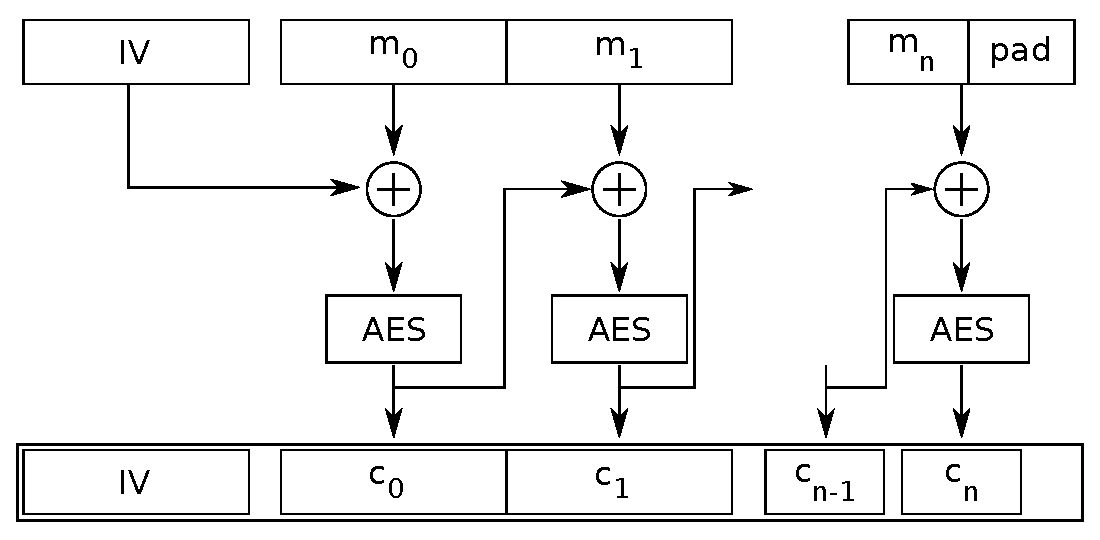
\includegraphics[scale=1]{cbc.eps}
 
\paragraph{Outline}
The remainder of this article is organized as follows.
Section~\ref{previous work} gives account of previous work.
Our new and exciting results are described in Section~\ref{results}.
Finally, Section~\ref{conclusions} gives the conclusions.

\section{Google App Engine}\index{Google App Engine}



\subsection{Handlers}\index{Google App Engine!Handlers}

\subsubsection{Regular handler}

\begin{Verbatim}[commandchars=\\\{\}]
\PY{k}{class} \PY{n+nc}{TestHandler}\PY{p}{(}\PY{n}{webapp2}\PY{o}{.}\PY{n}{RequestHandler}\PY{p}{)}\PY{p}{:}
  \PY{k}{def} \PY{n+nf}{get}\PY{p}{(}\PY{n+nb+bp}{self}\PY{p}{)}\PY{p}{:}
    \PY{n}{q} \PY{o}{=} \PY{n+nb+bp}{self}\PY{o}{.}\PY{n}{request}\PY{o}{.}\PY{n}{get}\PY{p}{(}\PY{l+s}{"}\PY{l+s}{q}\PY{l+s}{"}\PY{p}{)} \PY{c}{\PYZsh{}get parameter q}
    \PY{n+nb+bp}{self}\PY{o}{.}\PY{n}{response}\PY{o}{.}\PY{n}{out}\PY{o}{.}\PY{n}{write}\PY{p}{(}\PY{n}{q}\PY{p}{)}

\PY{n}{app} \PY{o}{=} \PY{n}{webapp2}\PY{o}{.}\PY{n}{WSGIApplication}\PY{p}{(}\PY{p}{[}\PY{p}{(}\PY{l+s}{'}\PY{l+s}{/}\PY{l+s}{'}\PY{p}{,}\PY{n}{MainPage}\PY{p}{)}\PY{p}{,}\PY{p}{(}\PY{l+s}{'}\PY{l+s}{/testform}\PY{l+s}{'}\PY{p}{,}\PY{n}{TestHandler}\PY{p}{)}\PY{p}{]}\PY{p}{,}\PY{n}{debug}\PY{o}{=}\PY{n+nb+bp}{True}\PY{p}{)}
\end{Verbatim}




\subsection{Forms}\index{Google App Engine!Forms}

\begin{Verbatim}[commandchars=\\\{\}]
\PY{n}{form}\PY{o}{=}\PY{l+s}{"""}
\PY{l+s}{  <form method=}\PY{l+s}{"}\PY{l+s}{post}\PY{l+s}{"}\PY{l+s}{>}
\PY{l+s}{  <label>Free Field <input name=}\PY{l+s}{"}\PY{l+s}{q}\PY{l+s}{"}\PY{l+s}{ value=}\PY{l+s}{"}\PY{l+s+si}{\PYZpc{}(q)s}\PY{l+s}{"}\PY{l+s}{></label> }
\PY{l+s}{  <div style=}\PY{l+s}{"}\PY{l+s}{color: red}\PY{l+s}{"}\PY{l+s}{>}\PY{l+s+si}{\PYZpc{}(error)s}\PY{l+s}{</div>}
\PY{l+s}{  </form>}
\PY{l+s}{"""}
\PY{k}{def} \PY{n+nf}{validation\PYZus{}function}\PY{p}{(}\PY{n}{q}\PY{p}{)}\PY{p}{:}
  \PY{n}{reutrn} \PY{o}{.}\PY{o}{.}\PY{o}{.}

\PY{k}{class} \PY{n+nc}{MainPage}\PY{p}{(}\PY{n}{webapp2}\PY{o}{.}\PY{n}{RequestHandler}\PY{p}{)}\PY{p}{:}
  \PY{k}{def} \PY{n+nf}{write\PYZus{}form}\PY{p}{(}\PY{n+nb+bp}{self}\PY{p}{,}\PY{n}{error}\PY{o}{=}\PY{l+s}{"}\PY{l+s}{"}\PY{p}{,}\PY{n}{q}\PY{o}{=}\PY{l+s}{"}\PY{l+s}{"}\PY{p}{)}\PY{p}{:}
    \PY{n+nb+bp}{self}\PY{o}{.}\PY{n}{response}\PY{o}{.}\PY{n}{out}\PY{o}{.}\PY{n}{write}\PY{p}{(}\PY{n}{form} \PY{o}{\PYZpc{}} \PY{p}{\PYZob{}}\PY{l+s}{'}\PY{l+s}{error}\PY{l+s}{'}\PY{p}{:}\PY{n}{error}\PY{p}{,}\PY{l+s}{'}\PY{l+s}{q}\PY{l+s}{'}\PY{p}{:}\PY{n}{q}\PY{p}{\PYZcb{}}\PY{p}{)}

  \PY{k}{def} \PY{n+nf}{get}\PY{p}{(}\PY{n+nb+bp}{self}\PY{p}{)}\PY{p}{:}
    \PY{n+nb+bp}{self}\PY{o}{.}\PY{n}{write\PYZus{}form}\PY{p}{(}\PY{p}{)}

  \PY{k}{def} \PY{n+nf}{post}\PY{p}{(}\PY{n+nb+bp}{self}\PY{p}{)}\PY{p}{:}
    \PY{n}{user\PYZus{}q} \PY{o}{=} \PY{n+nb+bp}{self}\PY{o}{.}\PY{n}{request}\PY{o}{.}\PY{n}{get}\PY{p}{(}\PY{l+s}{'}\PY{l+s}{q}\PY{l+s}{'}\PY{p}{)}
    \PY{n}{q}      \PY{o}{=} \PY{n}{validation\PYZus{}function}\PY{p}{(}\PY{n}{user\PYZus{}q}\PY{p}{)}
  
    \PY{k}{if} \PY{o+ow}{not} \PY{n}{q}\PY{p}{:}
      \PY{n+nb+bp}{self}\PY{o}{.}\PY{n}{write\PYZus{}form}\PY{p}{(}\PY{l+s}{"}\PY{l+s}{Invalid form.}\PY{l+s}{"}\PY{p}{,}\PY{n}{user\PYZus{}q}\PY{p}{)}
    \PY{k}{else}\PY{p}{:}
      \PY{n+nb+bp}{self}\PY{o}{.}\PY{n}{response}\PY{o}{.}\PY{n}{out}\PY{o}{.}\PY{n}{write}\PY{p}{(}\PY{l+s}{"}\PY{l+s}{Thanks! That}\PY{l+s}{'}\PY{l+s}{s totally valid!}\PY{l+s}{"}\PY{p}{)}
\end{Verbatim}


User input need to be esacped.

\begin{Verbatim}[commandchars=\\\{\}]
\PY{k+kn}{import} \PY{n+nn}{cgi}
\PY{k}{print} \PY{n}{cgi}\PY{o}{.}\PY{n}{escape}\PY{p}{(}\PY{l+s}{'}\PY{l+s}{"}\PY{l+s}{<b&ld>}\PY{l+s}{"}\PY{l+s}{'}\PY{p}{,}\PY{n}{quote}\PY{o}{=}\PY{n+nb+bp}{True}\PY{p}{)} 
\PY{c}{\PYZsh{}--> &quot;&lt;b&amp;ld&gt;&quot;}
\end{Verbatim}




\subsubsection{Redirection}\index{Google App Engine!Forms!Redirection}

With redirection one can reload the page without having resubmitting a form. It's also good practice to have distinct pages for forms and successes.



\subsection{Templates}\index{Google App Engine!Templates}

Install the \emph{jinja2} library

\begin{tabular}{l}
sudo easy\_install jinja2
\end{tabular}

and modify your \emph{app.yaml} file

\begin{Verbatim}[commandchars=\\\{\}]
\PY{n}{application}\PY{p}{:} \PY{o}{<}\PY{n}{username}\PY{o}{>}
\PY{n}{version}\PY{p}{:} \PY{l+m+mi}{1}
\PY{n}{runtime}\PY{p}{:} \PY{n}{python27}
\PY{n}{api\PYZus{}version}\PY{p}{:} \PY{l+m+mi}{1}
\PY{n}{threadsafe}\PY{p}{:} \PY{n}{true}

\PY{n}{libraries}\PY{p}{:}
\PY{o}{-} \PY{n}{name}\PY{p}{:} \PY{n}{jinja2}
  \PY{n}{version}\PY{p}{:} \PY{n}{latest}

\PY{n}{handlers}\PY{p}{:}
\PY{o}{-} \PY{n}{url}\PY{p}{:} \PY{o}{/}\PY{o}{.}\PY{o}{*}
  \PY{n}{script}\PY{p}{:} \PY{n}{asciichan}\PY{o}{.}\PY{n}{app}
\end{Verbatim}


Make a simple html file in your \emph{templates} directory

\begin{Verbatim}[commandchars=\\\{\}]
\PY{c+cp}{<!DOCTYPE html>}
\PY{n+nt}{<html}\PY{n+nt}{>}
  \PY{n+nt}{<head}\PY{n+nt}{>}
    \PY{n+nt}{<title}\PY{n+nt}{>}/ascii/\PY{n+nt}{</title>}
  \PY{n+nt}{</head>}

  \PY{n+nt}{<body}\PY{n+nt}{>}
    \PY{n+nt}{<h1}\PY{n+nt}{>}/ascii/\PY{n+nt}{</h1>}
  \PY{n+nt}{</body>}
\PY{n+nt}{</html>}
\end{Verbatim}


and write your main file

\begin{Verbatim}[commandchars=\\\{\}]
\PY{k+kn}{import} \PY{n+nn}{os}
\PY{k+kn}{import} \PY{n+nn}{webapp2}
\PY{k+kn}{import} \PY{n+nn}{jinja2}

\PY{n}{template\PYZus{}dir} \PY{o}{=} \PY{n}{os}\PY{o}{.}\PY{n}{path}\PY{o}{.}\PY{n}{join}\PY{p}{(}\PY{n}{os}\PY{o}{.}\PY{n}{path}\PY{o}{.}\PY{n}{dirname}\PY{p}{(}\PY{n}{\PYZus{}\PYZus{}file\PYZus{}\PYZus{}}\PY{p}{)}\PY{p}{,} \PY{l+s}{'}\PY{l+s}{templates}\PY{l+s}{'}\PY{p}{)}
\PY{n}{jinja\PYZus{}env} \PY{o}{=} \PY{n}{jinja2}\PY{o}{.}\PY{n}{Environment}\PY{p}{(}\PY{n}{loader} \PY{o}{=} \PY{n}{jinja2}\PY{o}{.}\PY{n}{FileSystemLoader}\PY{p}{(}\PY{n}{template\PYZus{}dir}\PY{p}{)}\PY{p}{,} \PY{n}{autoescape} \PY{o}{=} \PY{n+nb+bp}{True}\PY{p}{)}

\PY{k}{class} \PY{n+nc}{Handler}\PY{p}{(}\PY{n}{webapp2}\PY{o}{.}\PY{n}{RequestHandler}\PY{p}{)}\PY{p}{:}
  \PY{k}{def} \PY{n+nf}{write}\PY{p}{(}\PY{n+nb+bp}{self}\PY{p}{,}\PY{o}{*}\PY{n}{a}\PY{p}{,}\PY{o}{*}\PY{o}{*}\PY{n}{kw}\PY{p}{)}\PY{p}{:}
    \PY{n+nb+bp}{self}\PY{o}{.}\PY{n}{response}\PY{o}{.}\PY{n}{out}\PY{o}{.}\PY{n}{write}\PY{p}{(}\PY{o}{*}\PY{n}{a}\PY{p}{,}\PY{o}{*}\PY{o}{*}\PY{n}{kw}\PY{p}{)}

  \PY{k}{def} \PY{n+nf}{render\PYZus{}str}\PY{p}{(}\PY{n+nb+bp}{self}\PY{p}{,}\PY{n}{template}\PY{p}{,}\PY{o}{*}\PY{o}{*}\PY{n}{params}\PY{p}{)}\PY{p}{:}
    \PY{n}{t} \PY{o}{=} \PY{n}{jinja\PYZus{}env}\PY{o}{.}\PY{n}{get\PYZus{}template}\PY{p}{(}\PY{n}{template}\PY{p}{)}
    \PY{k}{return} \PY{n}{t}\PY{o}{.}\PY{n}{render}\PY{p}{(}\PY{n}{params}\PY{p}{)}

  \PY{k}{def} \PY{n+nf}{render}\PY{p}{(}\PY{n+nb+bp}{self}\PY{p}{,}\PY{n}{template}\PY{p}{,}\PY{o}{*}\PY{o}{*}\PY{n}{kw}\PY{p}{)}\PY{p}{:}
    \PY{n+nb+bp}{self}\PY{o}{.}\PY{n}{write}\PY{p}{(}\PY{n+nb+bp}{self}\PY{o}{.}\PY{n}{render\PYZus{}str}\PY{p}{(}\PY{n}{template}\PY{p}{,}\PY{o}{*}\PY{o}{*}\PY{n}{kw}\PY{p}{)}\PY{p}{)}

\PY{k}{class} \PY{n+nc}{MainPage}\PY{p}{(}\PY{n}{Handler}\PY{p}{)}\PY{p}{:}
  \PY{k}{def} \PY{n+nf}{get}\PY{p}{(}\PY{n+nb+bp}{self}\PY{p}{)}\PY{p}{:}
      \PY{n+nb+bp}{self}\PY{o}{.}\PY{n}{render}\PY{p}{(}\PY{l+s}{'}\PY{l+s}{front.html}\PY{l+s}{'}\PY{p}{)}

\PY{n}{app} \PY{o}{=} \PY{n}{webapp2}\PY{o}{.}\PY{n}{WSGIApplication}\PY{p}{(}\PY{p}{[}\PY{p}{(}\PY{l+s}{'}\PY{l+s}{/}\PY{l+s}{'}\PY{p}{,}\PY{n}{MainPage}\PY{p}{)}\PY{p}{]}\PY{p}{,}\PY{n}{debug}\PY{o}{=}\PY{n+nb+bp}{True}\PY{p}{)}
\end{Verbatim}




\subsection{CSS}\index{Google App Engine!CSS}

\begin{Verbatim}[commandchars=\\\{\}]
\PY{n}{application}\PY{p}{:} \PY{o}{<}\PY{n}{username}\PY{o}{>}
\PY{n}{version}\PY{p}{:} \PY{l+m+mi}{1}
\PY{n}{runtime}\PY{p}{:} \PY{n}{python27}
\PY{n}{api\PYZus{}version}\PY{p}{:} \PY{l+m+mi}{1}
\PY{n}{threadsafe}\PY{p}{:} \PY{n}{true}

\PY{n}{handlers}\PY{p}{:}
\PY{o}{-} \PY{n}{url}\PY{p}{:} \PY{o}{/}\PY{n}{static}\PY{o}{/}
  \PY{n}{static\PYZus{}dir}\PY{p}{:} \PY{n}{static}

\PY{o}{-} \PY{n}{url}\PY{p}{:} \PY{o}{/}\PY{o}{.}\PY{o}{*}
  \PY{n}{script}\PY{p}{:} \PY{n}{asciichan}\PY{o}{.}\PY{n}{app}
\end{Verbatim}




\subsection{Google App Engine Datastore}
\
\textbf{Entity.} Tables, where the columns aren't fixed, all have id fields and have a notion of parents/ancestors which is a relation to other entities.


\subsubsection{GQL}\index{Google App Engine!Google App Engine Datastore!GQL}

A simplified version of SQL, where all queries begins with \emph{select *}, there are no joins and all queries must be indexed.

\begin{Verbatim}[commandchars=\\\{\}]
\PY{n}{posts} \PY{o}{=} \PY{n}{db}\PY{o}{.}\PY{n}{GqlQuery}\PY{p}{(}\PY{l+s}{"}\PY{l+s}{select * from Post order by created desc}\PY{l+s}{"}\PY{p}{)}
\PY{n}{posts} \PY{o}{=} \PY{n}{Post}\PY{o}{.}\PY{n}{all}\PY{p}{(}\PY{p}{)}\PY{o}{.}\PY{n}{order}\PY{p}{(}\PY{l+s}{'}\PY{l+s}{-created}\PY{l+s}{'}\PY{p}{)} \PY{c}{\PYZsh{}same}
\PY{n}{posts} \PY{o}{=} \PY{n+nb}{list}\PY{p}{(}\PY{n}{posts}\PY{p}{)} \PY{c}{\PYZsh{}detach from query}
\end{Verbatim}



\subsubsection{Types}\index{Google App Engine!Google App Engine Datastore!Types}

\begin{list}{*}{
\setlength{\itemsep}{0pt}
\setlength{\parsep}{0pt}
\setlength{\topsep}{0pt}
\setlength{\partopsep}{0pt}
\setlength{\leftmargin}{2em}
\setlength{\labelwidth}{1.5em}
\setlength{\labelsep}{0.5em}
}
\item Integer
\item Float
\item String - $<$ 500 chars, can be indexed and sorted
\item Text - $>$ 500 chars, cannot be indexed or sorted
\item Date
\item Time
\item DateTime
\item Email
\item Link
\item PostalAddress
\end{list}

\begin{Verbatim}[commandchars=\\\{\}]
\PY{k+kn}{from} \PY{n+nn}{google.appengine.ext} \PY{k+kn}{import} \PY{n}{db}
\PY{k}{class} \PY{n+nc}{Post}\PY{p}{(}\PY{n}{db}\PY{o}{.}\PY{n}{Model}\PY{p}{)}\PY{p}{:}
  \PY{n}{subject} \PY{o}{=} \PY{n}{db}\PY{o}{.}\PY{n}{StringProperty}\PY{p}{(}\PY{n}{required}       \PY{o}{=} \PY{n+nb+bp}{True}\PY{p}{)}
  \PY{n}{content} \PY{o}{=} \PY{n}{db}\PY{o}{.}\PY{n}{TextProperty}\PY{p}{(}\PY{n}{required}         \PY{o}{=} \PY{n+nb+bp}{True}\PY{p}{)}
  \PY{n}{created} \PY{o}{=} \PY{n}{db}\PY{o}{.}\PY{n}{DateTimeProperty}\PY{p}{(}\PY{n}{auto\PYZus{}now\PYZus{}add} \PY{o}{=} \PY{n+nb+bp}{True}\PY{p}{)}
  \PY{n}{updated} \PY{o}{=} \PY{n}{db}\PY{o}{.}\PY{n}{DateTimeProperty}\PY{p}{(}\PY{n}{auto\PYZus{}now}     \PY{o}{=} \PY{n+nb+bp}{True}\PY{p}{)}
\end{Verbatim}



\subsubsection{Console}\index{Google App Engine!Google App Engine Datastore!Console}

Go to address: localhost:8080/\_ah/admin


\subsection{Cookies}

A small piece of (temporary) data, clientside enforced stored in the browser for a website. Generally one can store about 20 cookies per website, which is a browser limitation. The length of the cookie is limited to around 4 kb. It also has to be a direct match or a subset to a particular domain.

Good uses of cookies
\begin{list}{*}{
\setlength{\itemsep}{0pt}
\setlength{\parsep}{0pt}
\setlength{\topsep}{0pt}
\setlength{\partopsep}{0pt}
\setlength{\leftmargin}{2em}
\setlength{\labelwidth}{1.5em}
\setlength{\labelsep}{0.5em}
}
\item Storing login information
\item Storing small amounts of data to avoid hitting a database
\item tracking a user for ads
\item \textcolor{red}{storing user preferences info - NO, want data to survice}
\end{list}

One can change a cookie within the console in one's browser's development tools

\begin{tabular}{l}
document.cookie $\#$ "visits=6" \\
document.cookie="visits=10000"
\end{tabular}

Secure the cookie with a HMAC\index{Cookies!HMAC}

\begin{Verbatim}[commandchars=\\\{\}]
\PY{k+kn}{import} \PY{n+nn}{os}
\PY{k+kn}{import} \PY{n+nn}{webapp2}
\PY{k+kn}{import} \PY{n+nn}{jinja2}

\PY{k+kn}{from} \PY{n+nn}{google.appengine.ext} \PY{k+kn}{import} \PY{n}{db}

\PY{n}{template\PYZus{}dir} \PY{o}{=} \PY{n}{os}\PY{o}{.}\PY{n}{path}\PY{o}{.}\PY{n}{join}\PY{p}{(}\PY{n}{os}\PY{o}{.}\PY{n}{path}\PY{o}{.}\PY{n}{dirname}\PY{p}{(}\PY{n}{\PYZus{}\PYZus{}file\PYZus{}\PYZus{}}\PY{p}{)}\PY{p}{,} \PY{l+s}{'}\PY{l+s}{templates}\PY{l+s}{'}\PY{p}{)}
\PY{n}{jinja\PYZus{}env} \PY{o}{=} \PY{n}{jinja2}\PY{o}{.}\PY{n}{Environment}\PY{p}{(}\PY{n}{loader} \PY{o}{=} \PY{n}{jinja2}\PY{o}{.}\PY{n}{FileSystemLoader}\PY{p}{(}\PY{n}{template\PYZus{}dir}\PY{p}{)}\PY{p}{,} \PY{n}{autoescape} \PY{o}{=} \PY{n+nb+bp}{True}\PY{p}{)}

\PY{c}{\PYZsh{}-----------------------------------------}
\PY{c}{\PYZsh{}import hashlib}
\PY{k+kn}{import} \PY{n+nn}{hmac}
\PY{n}{SECRET} \PY{o}{=} \PY{l+s}{'}\PY{l+s}{secret}\PY{l+s}{'}

\PY{k}{def} \PY{n+nf}{check\PYZus{}secure\PYZus{}val}\PY{p}{(}\PY{n}{h}\PY{p}{)}\PY{p}{:}
  \PY{n}{val} \PY{o}{=} \PY{n}{h}\PY{o}{.}\PY{n}{split}\PY{p}{(}\PY{l+s}{'}\PY{l+s}{|}\PY{l+s}{'}\PY{p}{)}\PY{p}{[}\PY{l+m+mi}{0}\PY{p}{]}
  \PY{k}{if} \PY{n}{h} \PY{o}{==} \PY{n}{make\PYZus{}secure\PYZus{}val}\PY{p}{(}\PY{n}{val}\PY{p}{)}\PY{p}{:} \PY{k}{return} \PY{n}{val}

\PY{k}{def} \PY{n+nf}{hash\PYZus{}str}\PY{p}{(}\PY{n}{s}\PY{p}{)}\PY{p}{:}
  \PY{c}{\PYZsh{}return hashlib.md5(s).hexdigest()}
  \PY{k}{return} \PY{n}{hmac}\PY{o}{.}\PY{n}{new}\PY{p}{(}\PY{n}{SECRET}\PY{p}{,}\PY{n}{s}\PY{p}{)}\PY{o}{.}\PY{n}{hexdigest}\PY{p}{(}\PY{p}{)}

\PY{k}{def} \PY{n+nf}{make\PYZus{}secure\PYZus{}val}\PY{p}{(}\PY{n}{s}\PY{p}{)}\PY{p}{:}
  \PY{k}{return} \PY{l+s}{"}\PY{l+s+si}{\PYZpc{}s}\PY{l+s}{|}\PY{l+s+si}{\PYZpc{}s}\PY{l+s}{"} \PY{o}{\PYZpc{}} \PY{p}{(}\PY{n}{s}\PY{p}{,}\PY{n}{hash\PYZus{}str}\PY{p}{(}\PY{n}{s}\PY{p}{)}\PY{p}{)}
\PY{c}{\PYZsh{}-----------------------------------------}

\PY{k}{class} \PY{n+nc}{Handler}\PY{p}{(}\PY{n}{webapp2}\PY{o}{.}\PY{n}{RequestHandler}\PY{p}{)}\PY{p}{:}
  \PY{k}{def} \PY{n+nf}{write}\PY{p}{(}\PY{n+nb+bp}{self}\PY{p}{,}\PY{o}{*}\PY{n}{a}\PY{p}{,}\PY{o}{*}\PY{o}{*}\PY{n}{kw}\PY{p}{)}\PY{p}{:}
    \PY{n+nb+bp}{self}\PY{o}{.}\PY{n}{response}\PY{o}{.}\PY{n}{out}\PY{o}{.}\PY{n}{write}\PY{p}{(}\PY{o}{*}\PY{n}{a}\PY{p}{,}\PY{o}{*}\PY{o}{*}\PY{n}{kw}\PY{p}{)}

  \PY{k}{def} \PY{n+nf}{render\PYZus{}str}\PY{p}{(}\PY{n+nb+bp}{self}\PY{p}{,}\PY{n}{template}\PY{p}{,}\PY{o}{*}\PY{o}{*}\PY{n}{params}\PY{p}{)}\PY{p}{:}
    \PY{n}{t} \PY{o}{=} \PY{n}{jinja\PYZus{}env}\PY{o}{.}\PY{n}{get\PYZus{}template}\PY{p}{(}\PY{n}{template}\PY{p}{)}
    \PY{k}{return} \PY{n}{t}\PY{o}{.}\PY{n}{render}\PY{p}{(}\PY{n}{params}\PY{p}{)}

  \PY{k}{def} \PY{n+nf}{render}\PY{p}{(}\PY{n+nb+bp}{self}\PY{p}{,}\PY{n}{template}\PY{p}{,}\PY{o}{*}\PY{o}{*}\PY{n}{kw}\PY{p}{)}\PY{p}{:}
    \PY{n+nb+bp}{self}\PY{o}{.}\PY{n}{write}\PY{p}{(}\PY{n+nb+bp}{self}\PY{o}{.}\PY{n}{render\PYZus{}str}\PY{p}{(}\PY{n}{template}\PY{p}{,}\PY{o}{*}\PY{o}{*}\PY{n}{kw}\PY{p}{)}\PY{p}{)}

\PY{k}{class} \PY{n+nc}{MainPage}\PY{p}{(}\PY{n}{Handler}\PY{p}{)}\PY{p}{:}
  \PY{k}{def} \PY{n+nf}{get}\PY{p}{(}\PY{n+nb+bp}{self}\PY{p}{)}\PY{p}{:}
    \PY{n+nb+bp}{self}\PY{o}{.}\PY{n}{response}\PY{o}{.}\PY{n}{headers}\PY{p}{[}\PY{l+s}{'}\PY{l+s}{Content-Type}\PY{l+s}{'}\PY{p}{]} \PY{o}{=} \PY{l+s}{'}\PY{l+s}{text/plain}\PY{l+s}{'}
    \PY{n}{visits} \PY{o}{=} \PY{l+m+mi}{0}
    \PY{n}{visit\PYZus{}cookie\PYZus{}str} \PY{o}{=} \PY{n+nb+bp}{self}\PY{o}{.}\PY{n}{request}\PY{o}{.}\PY{n}{cookies}\PY{o}{.}\PY{n}{get}\PY{p}{(}\PY{l+s}{'}\PY{l+s}{visits}\PY{l+s}{'}\PY{p}{)}
    \PY{k}{if} \PY{n}{visit\PYZus{}cookie\PYZus{}str}\PY{p}{:}
      \PY{n}{cookie\PYZus{}val} \PY{o}{=} \PY{n}{check\PYZus{}secure\PYZus{}val}\PY{p}{(}\PY{n}{visit\PYZus{}cookie\PYZus{}str}\PY{p}{)}
      \PY{k}{if} \PY{n}{cookie\PYZus{}val}\PY{p}{:}
        \PY{n}{visits} \PY{o}{=} \PY{n+nb}{int}\PY{p}{(}\PY{n}{cookie\PYZus{}val}\PY{p}{)}
    \PY{n}{visits} \PY{o}{+}\PY{o}{=} \PY{l+m+mi}{1}
    \PY{n}{new\PYZus{}cookie\PYZus{}val} \PY{o}{=} \PY{n}{make\PYZus{}secure\PYZus{}val}\PY{p}{(}\PY{n+nb}{str}\PY{p}{(}\PY{n}{visits}\PY{p}{)}\PY{p}{)}
    \PY{n+nb+bp}{self}\PY{o}{.}\PY{n}{response}\PY{o}{.}\PY{n}{headers}\PY{o}{.}\PY{n}{add\PYZus{}header}\PY{p}{(}\PY{l+s}{'}\PY{l+s}{Set-Cookie}\PY{l+s}{'}\PY{p}{,}\PY{l+s}{'}\PY{l+s}{visits=}\PY{l+s+si}{\PYZpc{}s}\PY{l+s}{'} \PY{o}{\PYZpc{}} \PY{n}{new\PYZus{}cookie\PYZus{}val}\PY{p}{)}
    \PY{n+nb+bp}{self}\PY{o}{.}\PY{n}{write}\PY{p}{(}\PY{l+s}{'}\PY{l+s}{You}\PY{l+s+se}{\PYZbs{}'}\PY{l+s}{ve been here }\PY{l+s+si}{\PYZpc{}s}\PY{l+s}{ times}\PY{l+s}{'} \PY{o}{\PYZpc{}} \PY{n}{visits}\PY{p}{)}
    

\PY{n}{app} \PY{o}{=} \PY{n}{webapp2}\PY{o}{.}\PY{n}{WSGIApplication}\PY{p}{(}\PY{p}{[}\PY{p}{(}\PY{l+s}{'}\PY{l+s}{/}\PY{l+s}{'}\PY{p}{,}\PY{n}{MainPage}\PY{p}{)}\PY{p}{]}\PY{p}{,}\PY{n}{debug}\PY{o}{=}\PY{n+nb+bp}{True}\PY{p}{)}
\end{Verbatim}


\begin{tabular}{l}
document.cookie $\#$ "visits=6|295c82aceeb5f3715e6e3304199e1ae0" \\
\end{tabular}



\subsection{Database}

\subsubsection{Clear the database}

\begin{tabular}{l}
dev\_appserver.py --clear\_datastore .
\end{tabular}



\section{Qotes}

Ascii art. It's a fantastic way for people to waste their time in front of their keyboards. - Hoffman

If your data has structure, use Oracle. If your data has no structure, use Hadoop. If your data has no value, use MongoDB.

Time flies like an arrow, fruit flies like a banana.

Let's beat this dead horse a little big longer.

Before you embark on a journey of revenge, dig two graves. - Confucius (504 B.C.)

Beware of bugs in the above code. I have only proven it correct, not tried it. - Donald Knuth

Before you learn how to see, you must realize your are blind.


\bibliographystyle{abbrv}
\bibliography{main}

\printindex

\end{document}
